\documentclass[12pt, a4paper]{article}
\usepackage{amsmath}
%\usepackage{german}
%\usepackage[ngerman]{babel}
\usepackage{graphicx}
\usepackage[skip=5pt,font=scriptsize,justification=justified,singlelinecheck=false]{caption}
\usepackage{wrapfig}
\usepackage{float}
\usepackage{siunitx}
\usepackage{textcomp}
\usepackage{accents}
\usepackage{enumitem}
\usepackage{color}
\usepackage{comment} 
%\usepackage[version=3]{mhchem}
\usepackage{url}
\usepackage{pdfpages}
\usepackage{upgreek}
\usepackage{scrlayer-scrpage}
\pagestyle{scrheadings}
\usepackage{caption}
\usepackage{amsfonts}
\usepackage{physics}
\usepackage{hyperref}
\usepackage{pdfpages}
\usepackage{biblatex}
\usepackage{amssymb}
\usepackage{titlepic}
\usepackage{forest}
\usepackage[linesnumbered,ruled]{algorithm2e}
%\usepackage{algorithm}
%\usepackage{algorithmic}
%\usepackage{algcompatible}
\usepackage{algpseudocode}
\addbibresource{literatur.bib}
%\usepackage{subfigure}
\DeclareUnicodeCharacter{2212}{-}
\usepackage[labelfont={bf,sf},font={small},%
labelsep=space]{caption}
\usepackage{doi}
%%%%%%%%%%%%%%%%%%%%%%%%%%%%%%%%%%%%%%%%%%%%%%%%%%%%%%%%%%%%%%%%%%%
% Ein Makro für Bezug auf Abbildungen
\newcommand{\fref}[1]{\figurename\ \ref{#1}}
% Ein Makro für Bezug auf Seiten
\newcommand{\pref}[1]{\pagename\ \pageref{#1}}
% Ein Makro fuer Bezug auf eine Section
\newcommand{\sref}[1]{section\ \ref{#1}}
% Ein Makro fuer Bezug auf Zeile in Codelistings
\newcommand{\lref}[1]{Line\ \ref{#1}}
% Ein Makro fuer Bezug auf ein Listing
\newcommand{\Lref}[1]{Listing\ \ref{#1}}
% Ein Makro fuer Bezug auf Tabellen
\newcommand{\tref}[1]{\tablename\ \ref{#1}}
%%%%%%%%%%%%%%%%%%%%%%%%%%%%%%%%%%%%%%%%%%%%%%%%%%%%%%%%%%%%%%%%%%%%
\begin{document}

\ihead{Maximilian Gschaider}
    \chead{Gradient Boosting Machine}
    \ohead{16.10.2023}
\cfoot*{\pagemark}%

\newpage 
\thispagestyle{empty}

\newpage
\clearpage

\title{
Gradient Boosting Machine \\
based on Decision Tree Regressor \\
\large tuned by Bayesian Optimization \\
\vspace{1cm}\\
\textbf{Technical University Graz}\\
Institute of Theoretical and Computational Physics }
\author{
\\\\Maximilian Gschaider\\ \href{mailto:gschaider@student.tugraz.at}{gschaider@student.tugraz.at} \\
\vspace{1cm}\\
{\small Univ.-Prof. Dr. Wolfgang von der Linden \\
\small Advisor: Dr. Sascha Ranftl} }
\titlepic{\includegraphics[width=220]{figures/TU_Graz.png}}
\date{16.10.2023}
\maketitle
%\thispagestyle{empty}
%%%%%%%%%%%%%%%%%%%%%%%%%%%%%%%%%%%%%%%%%%%%%%%%%%%%%%%%%%%%%%%%%%%%%%%%%%%%
%%%%%%%%%%%%%%%%%%%%%%%%%%%%%%%%%%%%%%%%%%%%%%%%%%%%%%%%%%%%%%%%%%%%%%%%%%%%
\newpage
\section*{Abstract}
Gradient Boosting is a supervised machine learning technique which is used in regression and classification tasks. Because of its prediction speed, accuracy and interpretability especially with large and complex data structures it attracted a lot of attention in the last decades. It's a special kind of ensemble method where multiple learning models are combined to obtain better predictive performance than could be obtained from any of the constituent learning models alone. Through converting weak learners to strong ones one can benefit of the boosting structure. In comparison to Bootstrap Aggregating (bagging), Stacking or Voting the Gradient Boosting framework is built in a stage-wise fashion. Usually in regression tasks the weak learners are decision trees, because of its natural intelligibility and simplicity. Initially Schapire and Freund developed the first statistical meta-algorithm framework \textit{Adaboost}, an adaptive boosting algorithm that won the \textit{Gödel Prize}. The idea of gradient boosting originated in the observation by Leo Breiman that boosting can be interpreted as an optimization algorithm on a suitable cost function. The first explicit regression gradient boosting algorithms were subsequently developed by Jerome H. Friedman.
\clearpage
\thispagestyle{empty}
\tableofcontents
%%%%%%%%%%%%%%%%%%%%%%%%%%%%%%%%%%%%%%%%%%%%%%%%%%%%%%%%%%%%%%%%%%%%%%%%%%%%
%%%%%%%%%%%%%%%%%%%%%%%%%%%%%%%%%%%%%%%%%%%%%%%%%%%%%%%%%%%%%%%%%%%%%%%%%%%%
%%%%%%%%%%%%%%%%%%%%%%%%%%%%%%%%%%%%%%%%%%%%%%%%%%%%%%%%%%%%%%%%%%%%%%%%%%%%
%%%%%%%%%%%%%%%%%%%%%%%%%%%%%%%%%%%%%%%%%%%%%%%%%%%%%%%%%%%%%%%%%%%%%%%%%%%%
\newpage
\clearpage
\setcounter{page}{1}
%%%%%%%%%%%%%%%%%%%%%%%%%%%%%%%%%%%%%%%%%%%%%%%%%%%%%%%%%%%%%
%\newcommand\h{$h(\vec{x};\vec{a}_m)$}
%%%%%%%%%%%%%%%%%%%%%%%%%%%%%%%%%%%%%%%%%%%%%%%%%%%%%%%%%%%%%
\section{Introduction}

In the dynamic field of machine learning and predictive modeling, the search for accurate and efficient algorithms is a constant challenge. The quest for meaningful insights from data and accurate predictions has driven the development of increasingly sophisticated techniques. \\
Among these, Gradient Boosting Machines (GBM) have emerged as a powerful and versatile algorithm in the realm of supervised machine learning. \\
At the heart of the Gradient Boosting Machine lies the fusion of two fundamental concepts: \textit{ensemble learning} and \textit{decision trees}. Decision trees, being intuitive and interpretable, have been a powerful tool in the field of classification and regression tasks for decades. They partition data into subsets based on feature attributes and recursively make decisions, resulting in a tree-like structure that can provide valuable insights into the decision-making process. However, standalone decision trees often suffer from overfitting and suboptimal predictive performance. In response to these challenges, ensemble learning techniques have gained prominence. Gradient Boosting, in particular, has demonstrated exceptional capability in enhancing the predictive accuracy of decision trees. By iteratively building an ensemble of decision trees and adjusting their weights based on the errors made by the preceding trees, Gradient Boosting Machines can significantly improve predictive performance while mitigating overfitting concerns. \\
This thesis embarks on a comprehensive exploration of Gradient Boosting Machines built upon decision trees as a foundational framework. \\
The overarching objective of this study is to explore the synergy between Gradient Boosting with Decision Trees and Bayesian Optimization, merging the prowess of ensemble learning with informative hyperparameter tuning. In pursuit of this goal, I endeavor to accomplish the following key objectives:\\
\vspace{0.5cm} \\
\textbf{In-Depth algorithmic understanding:}  \\
Investigate the foundational principles of Gradient Boosting and Decision Tree Regressor, establishing a robust theoretical foundation for our proposed approach. 
\\
\textbf{Framework built from scratch:} \\
Construct a Gradient Boosting Machine grounded in Decision Tree Regressors. \\
\textbf{Model optimization:} \\
Implement Bayesian Optimization as a versatile and resilient optimization technique, adept at efficiently navigating and optimizing the hyperparameter landscape. 
\\
\textbf{Practical applications:} \\ 
Throughout this thesis, a practical test on a case study is presented and in addition a real-world data problem from the financial market is explored. \\
The corresponding Github repository can be viewed at the following link:
\href{https://github.com/probabilis/bs_ml}{Github Repository for BSc ML Project}. 
The project folder is structured as follows:
\vspace{0.5cm} \\
\begin{forest}
  for tree={
    font=\ttfamily,
    grow'=0,
    child anchor=west,
    parent anchor=south,
    anchor=west,
    calign=first,
    edge path={
      \noexpand\path [draw, \forestoption{edge}]
      (!u.south west) +(7.5pt,0) |- node[fill,inner sep=1.25pt] {} (.child anchor)\forestoption{edge label};
    },
    before typesetting nodes={
      if n=1
        {insert before={[,phantom]}}
        {}
    },
    fit=band,
    before computing xy={l=15pt},
  }
[bs\_ml
  [analysis]
  [bayesian\_opt]
  [figures]
  [from\_scratch]
  [gridsearch]
  [models]
  [preprocessing]
  [research]
  [rounds]
  [test]
  [test\_study]
  [tex]
  [...
    [main.py]
    [main\_neutralization.py]
    [repo\_utils.py]
    [requirements.txt]
  ]
]
\end{forest}

%%%%%%%%%%%%%%%%%%%%%%%%%%%%%%%%%%%%%%%%%%%%%%%%%%%%%%%%%%%%%%%%%%%%%%%%%%%%
\newpage
\section{Methodology}
The basic methodology and learning algorithms of GBM's algorithm, as originally derived by Friedman et al. \cite{Friedman2001} and Breiman et al. \cite{Breiman1984}. This overview is considered as an introduction and therefore the strict mathematical proofs of algorithms and their properties are not covered fully.
%%%%%%%%%%%%%%%%%%%%%%%%%%%%%%%%%%%%%%%%%%%%%%%%%%%%%%%%%%%%%%%%%%%%%%%%%%%%
\subsection{Function estimation}
In the function estimation or ``predictive learning`` problem, one has a system of ``input`` or ``explanatory`` variables $\vec{x} = \{x_1,...,x_n\}$ and a depending ``output`` or ``response`` variable $y$. The goal is to reconstruct the unknown functional dependence $\vec{x} \xrightarrow{F} y$ with the estimate $\tilde{F}(\vec{x})$, such that some specified loss function $L(y,F)$ is minimized.
\begin{center}
    $\tilde{F}(\vec{x}) = \underset{F(\vec{x})}{\arg\min} L(y,F(\vec{x}))$ 
\end{center}
By using this training sample $\{y,\vec{x_n}\}$ with the known $(y,\vec{x})$- values one can obtain an estimate or approximation $\tilde{F}(\vec{x})$ of the function $F(\vec{x})$ mapping $\vec{x}$ to $y$ which minimizes the expected value $\mathbb{E}$ of some specified loss function $L(y,F(\vec{x}))$ over the joint distribution of all $(y,\vec{x})$ -values:
\begin{equation}
    \tilde{F} = \underset{F}{\arg\min} \mathbb{E}_{y,\vec{x}} L(y,F(\vec{x})) = \underset{F}{\arg\min} \underbrace{\mathbb{E}_{\vec{x}} [\overbrace{\mathbb{E}_y (L(y,F(\vec{x})))}^\text{expected $y$ loss}|\vec{x}]}_\text{expectation over the whole dataset}
\end{equation}
Typically used loss functions (estimators) for regression problems $L(y,F)$ include squared-error $(y - F)^2$ and absolute-error $|y - F|$ for $y \in \mathbb{R}^1$.
Often the function to be determined $F(\vec{x})$ is restricted to be a member of a parameterized class of functions $F(\vec{x},\vec{P})$, where $\vec{P} = \{P_1,P_2,..\}$ is a discrete set of parameters whose joint values identify individual class members. Because of ''brave'' modelling behavior one can use only ``additive``` expansions of the form:
\begin{equation}
    F(\vec{x};\{\beta_m, \vec{a}_m\}_1^M) = \sum_{m=1}^{M} \beta_m h(\vec{x};\vec{a}_m)
    \label{eq: param_approx_function}
\end{equation}
The function $h(\vec{x};\vec{a}_m)$ is called a generic function (can handle different data types) and is usually a simple parameterized function of the input variables $\vec{x}$ by specific parameters $\vec{a} = \{a_1,a_2,...\}$. Depending on the joint values $\vec{a}_m$ chosen for these parameters the individual terms will differ. Expansions like (\ref{eq: param_approx_function}) are the basis of many function approximation methods such as neural networks or support vector machines. When working with a continuous domain of the variables the generic functions $h(\vec{x};\vec{a}_m)$ are often used as small regression trees, such as those produced by \textit{CART}$^{TM}$ [Ref. \cite{Breiman1984}]. For such regression trees the parameters $\vec{a}_m$ are the splitting variables, split locations and the terminal node means of the individual trees, but this will be discussed in section [\ref{sec: decision_trees}].
%%%%%%%%%%%%%%%%%%%%%%%%%%%%%%%%%%%%%%%%%%%%%%%%%%%%%%%%%%%%%%%%%%%%%%%%%%%%
\subsection{Numerical optimization}
By choosing a parameterized model $F(\vec{x};\vec{P})$ the function optimization problem becomes a parameter optimization problem:
\begin{equation}
    \label{eq: argmin_P}
    \tilde{\vec{P}} = \underset{P}{\arg\min} \Phi(\vec{P})
\end{equation}
where
\begin{center}
    $\Phi(\vec{P}) = \mathbb{E}_{y,\vec{x}} L(y,F(\vec{x};\vec{P})) $
\end{center}
is the risk function for the parameter optimization and $\mathbb{E}_{y,\vec{x}}$ defines the expectation over all output values $y$ and input vectors $\vec{x}$. From this it is evident that the following structure can be derived
\begin{center}
    $\tilde{F}(\vec{x}) = F(\vec{x};\tilde{\vec{P}})$
\end{center}
For most function estimations $F(\vec{x};\tilde{\vec{P}})$ and loss functions $L$ suitable numerical optimizations methods must be applied to solve (\ref{eq: argmin_P}). By expressing the solution for the parameters in the form 
\begin{equation}
    \label{eq: lc_par}
    \tilde{\vec{P}} = \sum_{m=0}^{M} \vec{p}_m
\end{equation}
of a linear combination, where $\vec{p}_0$ is an initial guess and $\{\vec{p_m}\}_1^M$ are successive increments (``steps`` or ``boosts``), each based on the sequence of preceding steps. The rule for computing of the individual steps $\vec{p}_m$ is defined by the specifically used optimization method.
%%%%%%%%%%%%%%%%%%%%%%%%%%%%%%%%%%%%%%%%%%%%%%%%%%%%%%%%%%%%%%
\subsection{Steepest-descent}
Steepest-descent is an unconstrained optimization technique and often used at numerical minimization methods. Therefore the increments $\{\vec{p}\}_1^M$ (\ref{eq: lc_par}) are defined as follows. First the current gradient $\vec{g}_m$ is computed:
\begin{center}
    $\vec{g}_m = \{g_{jm}\} = \nabla \Phi(\vec{P}) = \{ [\frac{\partial \Phi(\vec{P})}{\partial P_j}]_{\vec{P}=\vec{P}_{m-1}} \}$ with $\vec{P}_{m-1} = \sum_{m=0}^{m-1} \vec{p}_i$
\end{center}
The incremental step in the direction of the steepest-descent is taken to be
\begin{equation}
    \label{eq: gradient}
    \vec{p}_m = - \rho_m \vec{g}_m \text{with} \rho_m = \underset{\rho}{\arg\min} \Phi(\vec{P}_{m-1} - \rho \vec{g}_m).
\end{equation}
with a stepsize which results from the minimization of the parameterized solution with the evaluated steepest descent. Subsequently the ``steepest-descent`` is defined by the negative gradient \text{-}$\vec{g}_m$ direction (\ref{eq: gradient}) and is called the ``line search`` along that direction.
%%%%%%%%%%%%%%%%%%%%%%%%%%%%%%%%%%%%%%%%%%%%%%%%%%%%%%%%%%%%%%%%%%%%%%%%%%%%
\section{Numerical optimization in function space}
\label{sec: parameter_opt}
Let's first analyze the function estimation through numerical optimization in the ``nonparametric`` approach.
This is done by considering the initial function $F(\vec{x})$ is evaluated at each point $\vec{x}$ to be a ``parameter``, as Friedman et al. stated \cite{Friedman2001}. Consequently the following has to be minimized:
\begin{center}
    $\Phi(F) = \mathbb{E}_{y,\vec{x}} L(y,F(\vec{x}) = \mathbb{E}_{\vec{x}}[\mathbb{E}_y(L(y,F(\vec{x})))|\vec{x}]$
\end{center}
Whereby the expectation $\mathbb{E}_{y,\vec{x}}$ can be split up by chaining up the expectation $\mathbb{E}_{\vec{x}}$ with respect to the expectation $\mathbb{E}_y$ over the loss function given by the input vector $\vec{x}$. This can be shortened by evaluating directly at each individual $\vec{x}$ with respect to $F(\vec{x})$
\begin{center}
    $\Phi(F(\vec{x})) = \mathbb{E}_y [L(y,F(\vec{x}))|\vec{x}]$
\end{center}
Theoretically there are an infinite number of such parameters in function space, but in data sets are only a finite number $\{F(\vec{x}_i)\}_1^N$ given. Following the numerical optimization paradigm we take solutions to be 
\begin{center}
    $\tilde{F}(\vec{x}) = \sum_{m=0}^{M} f_m(\vec{x})$
\end{center}
where $f_0(\vec{x})$ is an initial guess and $\{f_m(\vec{x})\}_1^M$ are incremental functions (``steps`` or ``boosts``) defined by the optimization method. By using again the steepest-descent method the $m$-th incremental function results to
\begin{equation}
    \label{eq: incr_function}
    f_m(\vec{x}) = - \rho_m g_m(\vec{x})
\end{equation}
and with the definition of the gradient 
\begin{center}
    $g_m(\vec{x}) = [\frac{\partial \Phi(F(\vec{x}))}{\partial F(\vec{x})}]_{F(\vec{x}) = F_{m-1}(\vec{x})} = [\frac{\partial \mathbb{E}_y [L(y,F(\vec{x})|\vec{x}]}{\partial F(\vec{x})}]_{F(\vec{x}) = F_{m-1}(\vec{x})}$  
\end{center} 
and the total accumulation over all incremental functions 
\begin{center}    
    $F_{m-1} = \sum_{m=0}^{m-1} f_i(\vec{x})$
\end{center}
One can now assume that the following function suffices regularity and consequently differentiation and integration can be interchanged by integrating the expectation value $\mathbb{E}_y$ over the function values $F(\vec{x})$. 
\begin{equation}
    g_m(\vec{x}) = \mathbb{E}_y [\frac{\partial L(y, F(\vec{x}))}{\partial F(\vec{x})} | \vec{x}]_{F(\vec{x}) = F_{m-1}(\vec{x})}
\end{equation}
Again the factor $\rho_m$ in (\ref{eq: incr_function}) is given by the minimizing the line search
\begin{equation}
    \rho_m = \underset{\rho}{\arg\min} \mathbb{E}_{y,\vec{x}} L[y,F_{m-1}(\vec{x}) - \rho \vec{g}_m(\vec{x})]
\end{equation}
This represents the classical numerical optimization algorithm in function space, where one neglect parameterized solutions.
%%%%%%%%%%%%%%%%%%%%%%%%%%%%%%%%%%%%%%%%%%%%%%%%%%%%%%%%%
\newpage
\section{Barriers with finite data and GB design}
When dealing with a finite data-set the non-parametric approach breaks down because the joint distribution of $(y,\vec{x})$ is estimated only by this discrete set of data samples $\{y_i,\vec{x}_i\}_1^N$. This is because the expectation $\mathbb{E}_y[\cdot|\vec{x}]$ cannot be estimated accurately by its data value at each specific $\vec{x}_i$. Although it is not possible, one would also like to estimate $\tilde{F}(\vec{x})$ at $\vec{x}$ values other than the given training sample points.
Therefore strength and stability for the system must be borrowed from nearby data points by imposing smoothness on the solution. 
Friedman et al. supposed here an elegant way for providing a solution to this problem by assuming a parameterized form such as (\ref{eq: param_approx_function}) and performing a parameter optimization as discussed in section [\ref{sec: parameter_opt}] to minimize the corresponding data based estimate of the expected loss:
\begin{center}
    $\{\beta_m,\vec{a}_m\}_1^M = \underset{ \{\beta'_m,\vec{a}'_m \} }{\arg\min} 
    \sum_{i=1}^N L
    \left(y_i,\sum_{m=1}^M\beta'_{m} h(\vec{x}_i;\vec{a}'_m)\right)$
\end{center}
Due the fact that the summation over all $m$ in the argument of the loss function will be computationally impractical a ``greedy-stagewise`` approach will be implemented. Therefore for $m$ = 1,2,...,$M$ the following simplification will be used for optimizing the loss function
\begin{equation}
    \label{eq: greedy_stagewise}
        \{\beta_m,\vec{a}_m\} = \underset{ \{\beta,\vec{a} \} }{\arg\min} 
    \sum_{i=1}^N L
    (y_i,F_{m-1}(\vec{x_i}) + \beta h(\vec{x}_i;\vec{a}))
\end{equation}
for evaluating the stagewise function 
\begin{equation}
    F_m(\vec{x}) = F_{m-1}(\vec{x}) + \beta_m h(\vec{x};\vec{a}_m).
\end{equation}
It's definitely visible that by taking the last evaluated approximation instead of all generic functions in the evaluation of the loss function one gets a more efficient minimization calculation.
It must be noted that this \textit{stagewise} strategy is different from a stepwise approach that reconfigure previously entered terms when new ones are added. The function $h(\vec{x};\vec{a}_m)$ is called a ``weak`` or ``base learner``. \\
In addition it can be assumed that for a particular loss $L(y,F)$ and base learner $h(\vec{x};\vec{a}_m)$ the solution to (\ref{eq: greedy_stagewise}) is difficult to obtain, like Friedman mentioned in his official paper.
\\
\textit{Given any approximator $F_{m-1}(\vec{x})$ the function $\beta_m h(\vec{x};\vec{a})$ can be viewed the best greedy step towards the data based estimate of $\tilde{F}(\vec{x})$, under the constraint that the step ``direction`` $h(\vec{x};\vec{a}_m)$ be a member of the parameterized class of functions $h(\vec{x};\vec{a})$}, as Friedman et al. stated \cite{Friedman2001}. It can therefore be considered the steepest descent under that constraint. By the general construction, the data-based analogue of the unconstrained negative gradient,
\begin{center}
    $- g_m(\vec{x}_i) = - [\frac{\partial L(y_i, F(\vec{x}_i))}{\partial F(\vec{x}_i)}]_{F(\vec{x}) = F_{m-1}(\vec{x})}$
\end{center}
gives the best steepest-descent step direction $-\vec{g}_m = \{-g_m(\vec{x}_i\}_1^N$ in the $N$-dimensional data space at $F_{m-1}$.
But this gradient is defined only at the data points $\{\vec{x}_i\}_1^N$ and cannot be generalized to other $\vec{x}$-values. 
To bypass this limitation one can generalize the solution by choosing that member of the parameterized class $h(\vec{x};\vec{a}_m)$ that produces $\vec{h}_{m} = \{h(\vec{x}_i ;\vec{a})\}_1^N$ most parallel to $-\vec{g}_m \in \mathbb{R}^N$. \textit{This is the $h(\vec{x};\vec{a})$ most highly correlated with $- g_m(\vec{x})$ over the data distribution}, as Friedman et al. \cite{Friedman2001} proposed. This workaround for gaining information about the gradient can be obtained from the minimization of the solution:
\begin{equation}
    \vec{a}_m = \underset{ \vec{a}, \beta }{\arg\min} 
    \sum_{i=1}^N [- g_{m}(\vec{x_i}) - \beta h(\vec{x}_i;\vec{a})]^2
\end{equation}
\textit{This constrained negative gradient $h(\vec{x};\vec{a})$ is used in place of the unconstrained one $-\vec{g}_m(\vec{x})$ in the steepest-descent strategy}. Afterwards the line search is evaluated in respect to the minimization criteria
\begin{equation}
        \rho_m = \underset{\rho}{\arg\min} \sum_{i=1}^N L[y_i,F_{m-1}(\vec{x}_i) + \rho h(\vec{x}_i;\vec{a}_m)]
\end{equation}
and then the approximation updated
\begin{equation}
    F_{m} = F_{m-1}(\vec{x}) + \rho_m h(\vec{x};\vec{a}_m)
\end{equation}
\textit{Basically, instead of obtaining the solution under a smoothness constraint, the constraint is applied to the unconstrained (rough) solution by fitting $h(\vec{x};\vec{a})$ to the ``pseudo-responses`` $\{\tilde{y}_i = - g_m(\vec{x}_i)\}_{i=1}^N$} (quadratic deviation from the real gradient to the pseudo-gradient).
\textit{This permits the replacement of the difficult function minimization problem by least-squares function minimization, followed by only a single parameter optimization based on the original criterion}, as stated by Friedman et al. \cite{Friedman2001}.\\
So for any base learner function $h(\vec{x};\vec{a})$ for which a implementable least-squares algorithm exists for solving, one can use this approach to minimize any differentiable loss or objective function $L(y,F)$.
As shown, this is achieved with a forward stage-wise additive modeling method by using steepest-descent. 
\begin{algorithm}
\caption{Gradient Boosting}
\label{alg: gb_algo}
    $F_0(\vec{x}) = \underset{\rho}{\arg\min} \sum_{i=1}^N L(y_i,\rho)$ \\
    \For{$m = 1$ to $M$}
    {$\tilde{y}_i = [\frac{\partial L(y_i, F(\vec{x}_i))}{\partial F(\vec{x}_i)}]_{F(\vec{x}) = F_{m-1}(\vec{x})} \qquad i = 1,..,N$
    $\vec{a}_m = \underset{ \vec{a}, \beta }{\arg\min} 
    \sum_{i=1}^N [\tilde{y}_i - \beta h(\vec{x}_i;\vec{a})]^2$
    $\rho_m = \underset{\rho}{\arg\min} \sum_{i=1}^N L[y_i,F_{m-1}(\vec{x}_i) + \rho h(\vec{x}_i;\vec{a}_m)]$
    $F_{m} = F_{m-1}(\vec{x}) + \rho_m h(\vec{x};\vec{a}_m)$
    }
\end{algorithm}
In general any fitting criterion be used that estimates the conditional expectation (given $\vec{x}$) to evaluate the (smooth) negative gradient at line 3 of the Gradient Boosting Generic Algorithm [Alg. \ref{alg: gb_algo}].
Because of the universal and efficient computational properties of least-squares implementations one will select it when dealing with regression tasks.
%%%%%%%%%%%%%%%%%%%%%%%%%%%%%%%%%%%%%%%%%%%%%%%%%
\newpage
\section{Loss function and additive modeling}
In mathematical optimization a loss function is a function that maps an event or values of one or more variables onto a real number intuitively representing some ``cost`` associated with the event. Through optimization one can seek to minimize the loss function. In this paper we will focus only on quadratic loss-functions, because of the usability in regression tasks.
%%%%%%%%%%%%%%%%%%%%%%%%%%%%%%%%%%%%%%%%%%%%%%%%%
\subsection{Least-squares regression}
Defining the loss function as $L(y,F) = \frac{1}{2} (y - F)^2$ results in quadratic residuals with symmetric properties. Therefor the ``pseudo-responses`` in line 3 of the GB-algorithm [\ref{alg: gb_ls_algo}] results to $\tilde{y}_i = y_i - F_{m-1}(\vec{x}_i)$. The minimization in the following line results in fitting the current residuals and the line search produces the result $\rho_m = \beta_m$, where the parameter minimization of $\beta_m$ is already included when calculating $\vec{a}_m$. This results in the classical gradient boosting algorithm with least-squares regression which follows the usual stagewise approach by iteratively fitting the current residuals.
\begin{algorithm}
\caption{Gradient Boosting with least-squares regression}
\label{alg: gb_ls_algo}
    $F_0(\vec{x}) = \bar{y}$ \\
    \For{$m = 1$ to $M$}
    {
    $\tilde{y}_i = y_i - F_{m-1}(\vec{x}_i) \qquad i = 1,..,N$
    $\{\rho_m, \vec{a}_m \} = \underset{ \vec{a}, \rho }{\arg\min} 
    \sum_{i=1}^N [\tilde{y}_i - \rho h(\vec{x}_i;\vec{a})]^2$
    $F_{m} = F_{m-1}(\vec{x}) + \rho_m h(\vec{x};\vec{a}_m)$
    }
\end{algorithm}

\newpage
\subsection{Decision trees}
A regression tree is a tree model where the target variable can take continuous values. More generally, the concept of regression tree can be extended to any kind of object equipped with pairwise dissimilarities such as categorical sequences. The \textbf{term classification and regression tree (CART)} analysis is an umbrella term used to refer either regression or classification predictions [Ref. \cite{Dan2009}]. Gradient boosting because of its ensemble properties creates multiple decision trees based on the given hyperparameters. By incrementally building an ensemble by training each new instance to emphasize the training instances previously mismodeled.  \\
A decision tree is a simple representation for classifying examples. Assume that all the input features $\vec{x} = \{x_1,...,x_n\}$ have finite discrete domains and there's a single target feature $C_y$ called the ``classification``. 
Each element of the domain of the classification is called a ``class``. A decision tree is a tree in which each internal (non-leaf) node is labeled with an input feature. The links coming from a node labeled with an input feature are labeled with each of the possible values of the target feature or the link leads to a subordinate decision node on a different input feature. Each leaf of the tree is labeled with a class or a probability distribution over the classes, signifying that the dataset has been classified by the tree into either a specific class, or into a particular probability distribution. 
The tree is built by splitting the source set, constituting the root node of the tree, into subsets, which constitute the successor children.\\
The splitting is based on a set of splitting rules based on the inherent nature of features (regression or classification task). This process is repeated on each derived subset in a recursive manner called recursive partitioning. The recursion is completed when the subset at a node has all the same values of the target variable $y$ or when splitting no longer adds value to the predictions. This process of ``top-down induction of decision trees`` is an example of a greedy algorithm and it is by far the most common strategy for learning decision trees from data.
\begin{center}
$\mathcal{D} = \{(x^{(i)},y_i)\}_{i=1}^n$ is the training's data-set with input variables $x^{(i)} = (x_1^{i} ,...,x_n^{i}) \in \mathcal{X}$ and output variables $y \in \mathcal{Y}$.
\end{center}

\subsubsection{Regression tree}
\label{sec: decision_trees}
There are different algorithms for constructing decision trees by choosing a variable at each step that best splits the set of items. These generally measure the ``homogeneity`` of the target variable within the subsets. Depending on the discrete or continuous properties of the data-set one can use different metrics like positive correctness, gini-impurity, information gain, variance reduction or measure of goodness. \\
Introduced in CART, variance reduction is often used where the target variable is continuous ($\mathcal{Y} \subseteq \mathbb{R}$), so the output has quantitative properties.\\
A decision tree $T$ is presentable via a function $f_T : \mathcal{X} \rightarrow \mathcal{Y}$ which assigns each input a prediction of the output. The CART algorithm finds self-reliant the branches (nodes) and splitting rules for optimal allocation. 
As stated one can use different metrics for calculating the information gain.
We'll focus on the mean square root deviation for the error function,
\begin{center}
    $E(T,\mathcal{D}) = \frac{1}{m} \sum_{i=1}^m (f_T(x^{(i)}) - y_i)^2$
\end{center}
which has then be minimized. For each leaf $l$ a subset $R_l$ will be assigned, that for each $L$ leafs associated disjoint sets form a partition of $D$. One can now search an estimated value for all $x^{(i)} \in \mathcal{R}_l$ that best approximates the true value $\{y_i | x^{(i)} \in R_l\}$. 
The estimator 
\begin{center}
    $f_T(x^{(i)} \in R_l) = \mathbb{E}[y_i | x^{(i)} \in R_l] = \hat{c}_l$
\end{center}
provides a solution. Because the computational effort for calculation all possible trees is not efficient feasible one can use again a greedy algorithm. 
\textit{
One starts with a tree which consists of only one node and then successively find locally optimal branching.
} as Steinberg stated in his official paper \cite{Dan2009}.
At each node the individual property $j$ will be calculated which splits the entry in two disjoint regions of the parent nodes the best. For non-ordinal features (similarly to non-categorical) one can use the following metric:
\begin{equation}
    \underset{ j,s }{\min} \left( 
    \underset{ c_1 }{\min} 
    \sum_{x^{(i)} \in R_1(j,s)} (y_i - c_1)^2 + 
    \underset{ c_2 }{\min} 
    \sum_{x^{(i)} \in R_2(j,s)} (y_i - c_2)^2
    \right)
\end{equation}
Whereby $\hat{c}_k = \mathbb{E}[y_i | x^{(i)} \in R_k(j,s)]_{k = 1,2}$ in each case minimizes the two sums. Based on the single node each step two new nodes will be added which in turn are branched further until a termination condition (e.g.: the maximum path length from root to leaves / = max tree depth) is met. 
When having multiple features $\vec{x}_i$ as input, we can also us this relative rank (i.e. depth) of a feature to assess the relative importance of it with respect to the predictability of the target variable. Features used at the top of the tree contribute to the final prediction decision of a larger fraction of the input samples. The expected fraction of the samples they contribute to can thus be used as an estimate of the relative importance of the features. \\
In the following there's a simplified tree-growing algorithm from sketch given [Alg. \ref{alg: tree_growing_algo}]:
\begin{algorithm}
\caption{Simplified tree-growing algorithm sketch}\label{alg: tree_growing_algo}
    Assign all training data to the root node \\
    Define the root node as a terminal node \\
    \underline{SPLIT:} \\
    $NewSplits \gets 0$ \\
    \For{every terminal node in the tree}
    {
        \eIf{the terminal node sample size is too small or all instances in the node belong to the same target class}
        {\textbf{end}}
        {Find the attribute that best separates the node into two child nodes using an allowable splitting rule}
        $NewSplits \gets NewSplits + 1$\;
    }
\end{algorithm}
\newpage
So decision trees are very ``natural`` constructions, in particular when explanatory variables are categorical (and even better, when they're binary). Another advantage is that the created models are invariant under transformations in the predictor space, as Breiman et al. \cite{Breiman1984} stated. 
%%%%%%%%%%%%%%%%%%%%%%%%%%%%%%%%%%%
\subsubsection{Regression boosted trees}
\label{sec: regr_boosted_trees}
Let's combine these two concepts of \textit{Gradient Boosting} with the \textit{Decision Trees} as base learners, as Friedman et al. \cite{Friedman2001} proposed in his paper. \\
For simplification we consider the special case where each base learner is an $J$-terminal node regression tree [Ref. \cite{Breiman1984}]. Each regression tree model itself has the additive form 
\begin{equation}
    h(\vec{x};\{b_j,R_j\}_1^J) = \sum_{j=1}^J b_j \mathds{1}(\vec{x} \in R_j)
\end{equation}
Here $\{R_j\}_1^J$ are disjoint regions that collectively cover the space of all joint values of the predictor variables $\vec{x}$ \cite{Friedman2001}. These regions are represented by the terminal nodes of the corresponding tree. The indicator function $\mathds{1}$ has the value 1 if its argument is true and zero otherwise. The ``parameters`` of this base learner are the coefficients $\{b_j\}_1^J$ and the quantities that define the boundaries of the regions $\{R_j\}_1^J$. These are the splitting variables and the values of those variables that represent the splits at the non-terminal nodes of the tree. Because of the regions are disjoint is equivalent to the prediction rule: if $\vec{x} \in R_j$
then $h(\vec{x}) = b_j$.
For a regression tree the updating process of $F_m$ in the GB-algorithm [Alg. \ref{alg: gb_algo}] becomes
\begin{equation}
    F_m(\vec{x}) = F_{m-1}(\vec{x}) + \rho_m \sum_{j=1}^J b_{jm} \mathds{1}(\vec{x} \in \mathbb{R}_{jm})
\end{equation}
Here $\{R_{jm})\}_1^J$ are the regions defined by the terminal nodes of the tree at the $m$-th iteration. They are constructed to predict the pseudo-responses $\{\tidle{y}\}_1^N$ (line 3) by least-squares [Alg. \ref{alg: gb_algo}]. The $\{b_{jm}\}$ are the corresponding least-squares coefficients,
\begin{center}
    $b_{jm} = \mathbb{E}_{\vec{x}_i \in R_{jm}}[\tilde{y}_i]$
\end{center}
The scaling factor $\rho_m$ is again the solution to the ``line search`` [Alg. \ref{alg: gb_algo}].
The forward iteration can be also expressed as 
\begin{equation}
        F_m(\vec{x}) = F_{m-1}(\vec{x}) + \sum_{j=1}^J \gamma_{jm} \mathds{1}(\vec{x} \in R_{jm})
\end{equation}
with the coefficients $\gamma_{jm} = \rho \cdot b_{jm}$. This can be viewed as adding $J$ separate basis functions at each step $\{\mathds{1}(\vec{x} \in R_{jm})\}_1^J$ instead of a single additive one. By using the optimal coefficients for each of these separate basis functions  one can further improve the quality of the fit.
These coefficients are the solution to 
\begin{center}
    $\{\gamma_{jm}\}_1^J = \underset{\{\gamma_j\}_1^J}{\arg\min} \sum_{i=1}^N L\left(y_i,F_{m-1}(\vec{x}_i) + \sum_{j=1}^J \gamma_j \mathds{1}(\vec{x} \in R_{jm})\right)$
\end{center}
\textit{Owing to the disjoint nature of the regions produced by regression trees this reduces to}
\begin{equation}
        \label{eq: gamma_jm}
        \gamma_{jm} = \underset{\gamma}{\arg\min} \sum_{\vec{x}_i \in R_{jm}} L\left(y_i,F_{m-1}(\vec{x}_i) + \gamma\right)
\end{equation}
as Friedman \cite{Friedman2001} derived.
\textit{This is just the optimal constant update in each terminal node region, based on the loss function $L$ given the current approximation $F_{m-1}(\vec{x})$}. For the case of using LSD (least-squares deviation) regression (\ref{eq: gamma_jm}) becomes 
\begin{center}
    $\gamma_{jm} = \mathbb{E}_{\vec{x}_i \in R_{jm}}[y_i - F_{m-1}(\vec{x}_i)]$
\end{center}
which is simply the arithmetic mean of the current residuals in the $j$-th terminal node at the $m$-th iteration. At each iteration a regression tree is built to best predict the sign of the current residuals $y_i - F_{m-1}(\vec{x}_i)$ based on a least-squared criterion. Then the approximation is updated by adding the \textit{arithmetic mean} of the residuals in each of the derived terminal nodes.
\begin{algorithm}
\caption{LSD Tree-Boost}\label{alg: lsd_tree_boost_algo}
    $F_0(\vec{x}) = \text{mean}\{y_i\}_1^N$ \\
    \For{$m = 1$ to $M$}
    {
    $\tidle{y}_i = \sum_{i=1}^N [y_i - F_{m-1}(\vec{x})]^2$
    $\{R_{jm}\} = J-\text{terminal node } tree(\{\tilde{y}_i,\vec{x}_i\}_1^N$
    $\gamma_{jm} = \mathbb{E}_{\vec{x}_i \in R_{jm}}[y_i - F_{m-1}(\vec{x}_i)] , j = 1,..,J$
    $F_m(\vec{x}) = F_{m-1}(\vec{x}) + \sum_{j=1}^J \gamma_{jm} \mathds{1}(\vec{x} \in R_{jm})$
    }
\end{algorithm}
The trees use only order information on the individual input variables $\vec{x}_j$ and the pseudoresponses $\tilde{y}_i$ have a discrete set of values compared to the least-absolute deviation error function (LAD) where the output would be strict binary. Therefore the terminal node updates are based on the mean.
\newpage
\subsection{Regularization}
When predicting an output through fitting the training data too closely one can get a problem with overfitting the model. Reducing the expected loss on the training data beyond some point causes the prediction-expected loss to stop decreasing and often to start increasing again. 
Regularization methods attmept to prevent such ``overfitting`` by constraining the fitting procedure, as Friedman et al. \cite{Friedman2001} proposed originally.
For additive expansions a natural regularization parameter is the number of components $M$. This is similar to stepwise regression where the $\{h(\vec{x};\vec{a}_m)\}_1^M$ are considered explanatory variables that are sequentially entered. Through the adjustment of $M$ the regularization degree to which expected loss on the training data can be minimized. The best value for $M$ can be estimated by some model selection method such as cross-validation (CV) by \textit{Gridsearch}- or \textit{Bayesian-Optimization}. \\
\textit{Regularizing by controlling the number of terms in the expansion places an
implicit prior belief that ``sparse`` approximations involving fewer terms are
likely to provide better prediction. However, it has often been found that regularization through shrinkage provides superior results to that obtained by
restricting the number of components [Copas (1983)]}, as Friedman \cite{Friedman2001} described.
When working with additive models in a forward stagewise manner a simple shrinkage strategy is to replace the last line of the generic algorithm [Alg. \ref{alg: gb_algo}] with
\begin{equation}
    \label{eq: gb_algo_shrinkage}
    F_m(\vec{x}) = F_{m-1}(\vec{x}) + \nu \cdot \rho_{m} h(\vec{x};\vec{a}_m) \qquad 0 < \nu \leq 1
\end{equation}
(equally for all other algorithms). Consequentially each update is simply scaled down by the value of the ``learning rate`` parameter $\nu$.
Introducing shrinkage into gradient boosting (\ref{eq: gb_algo_shrinkage}) in this manner provides two regularization parameters, the learning rate $\nu$ and the number of components $M$. Each one can control the degree of fit and thus affect the best value for the other one. Decreasing the value $\nu$ increases the best value for $M$. Ideally one should estimate optimal values for both by minimizing a model selection criterion jointly with respect to the values of the two parameters. But one has to consider the proportional increase in computation when increasing the size of $M$.
%%%%%%%%%%%%%%%%%%%%%%%%%%%%%%%%%%%%%%%%%%%%%%%%%%%%%
\newpage
\section{Cross validation}
\label{sec: cross_validation}
Cross validation or out-of-sample testing is any of various similar model validation techniqes for assesing how to results of a statistical analysis will generalize to an independent data set. It is a resampling method that uses different portions of the data to test and train a model in different iterations. It is mainly used in settings where the goal is prediction and one wants to estimate how accurately a predictive model will perform in practice. Usually one have a dataset of \textit{known data} on which training is run (training dataset) and a dataset of \textit{unknown data} against which the model is tested (validation dataset).
Therefore the goal of cross-validation is to test the model's ability to predict new data what was not used in estimating it in order to flag problems like overfitting or selection bias. \\
One round of cross-validation involves partitioning a sample of data into complementary subsets, performing the analysis on the training set and validating the analysis on the validation set.
To reduce variability in most methods multiple rounds of cross-validation are performed using different partitions. So to sum up CV averages measures of fitness in prediction to derive a more accurate estimate of model prediction performance via a specific metric. \\
There are two types of cross validation methods which have to be distinguished: \textit{exhaustive} and \textit{non-exhaustive} strategies. An exhaustive cross-validation method learns and tests on all possible ways to divide the original sample into training and validation set. Non-exhaustive cross validation methods do not compute all ways of splitting the original sample. These methods are approximations of leave-$p$-out cross-validation.
%%%%%%%%%%%%%%%%%%%%%%%%%%%%%%%%%%%%%%%%%%%%%%%%
\subsection{$k$-fold cross-validation}
In $k$-fold cross-validation (non-exhaustive) the original sample is randomly partitioned into $k$ equal size subsamples.
Of the $k$ subsamples, a single subsample is retrained as the validation data for testing the model and the remaining $k - 1$ subsamples are used as training data. This cross validation process is then repeated $k$ times with each of the $k$ subsamples used exactly once as the validation data. The $k$ results can then be averaged to produce a single estimation. One advantage of this method over repeated random sub-sampling is that all observations are used for both training and validation and each observation is used for validation exactly once. In the figure below is a typical flowchart visible for model training [Fig. \ref{fig: cv_flowchart}]. \\
The dataset gets split up for training and testing (validation) the built model and with the training set one can obtain the best parameter constellation via cross-validation metrics. With the retrained model on the best parameters based on some scoring metric one can finally use the trained model to predict on new data.
\begin{figure}[!htpb]
    \centering
    \includegraphics[width=0.7\textwidth,trim={0 0 0 0},clip]{figures/cv_flowchart.png}
    \caption[Flowchart of model training]{Flowchart of model training and testing via cross-validation [\href{https://scikit-learn.org/stable/modules/cross_validation.html}{Scikit}]}
    \label{fig: cv_flowchart}    
\end{figure}
In most data science problems the initial dataset consists only of training data. The model is trained using $k - 1$ of the folds as training data and the resulting model is validated on the remaining part of the data [\ref{fig: cv_flowchart}].
The performance measure reported by $k$-fold cross validating is then the average of the values computed in the loop. 
After initializing the hyper-parameters of the framework one can cross-validate the training set and choose more suitable ones by comparing the models.
Usually the best parameters for a given gradient boosting framework are determined by uninformed gridsearch or informed bayesian optimization frameworks.
\begin{figure}[!htpb]
    \centering
    \includegraphics[width=0.6\textwidth,trim={0 0 0 0},clip]{figures/grid_search_cross_validation.png}
    \caption[Gridsearch by cross validation parameter evaluation]{Gridsearch by $k$-cross validation parameter evaluation [\href{https://scikit-learn.org/stable/modules/cross_validation.html}{Scikit}]}
    \label{fig: cv_flowchart}    
\end{figure}
%%%%%%%%%%%%%%%%%%%%%%%%%%%%%%%%%%%%%%%%%%%%%%%%%%
\subsection{Uninformed cross-validation / Gridsearch}
Given a boosting framework with hyperparameters $\{p_1,...,p_n\}$ to tune one can use the uninformed gridsearch framework to determine the highest score of performance of the underlying model. \\
The gridsearch method spans an $n$-dimensional space of the given hyperparameters with predefined boundaries of the given parameter interval and exhaustively generates candidates from a grid of parameter values specified.
The gridsearch cross validation framework implements the usual estimator API: when ``fitting`` it on a dataset all the possible combinations of parameter values are evaluated and the best combination is retained.
One could also use a randomized search cross validation framework. Random search tries randomly chosen combinations of a range of values where the number of iterations have to be defined beforehand. The problem here is that there's no guarantee that the output includes the best hyperparameter combination. Consequently one can say the gridsearch method is a directed method with predefined process flow in contrast to random search which randomly choose the grid point and do not learn from prior information. To prevent this an informed cross validation strategy can be used like bayesian optimization.
%%%%%%%%%%%%%%%%%%%%%%%%%%%%%%%%%%%%%%%%%%%%%%%%%%
\subsection{Informed cross-validation / Bayesian Optimization}
\label{sec: bayesian_opt}
As stated in the uninformed parameter optimization approach the idea is of developing automatic approaches which can optimize the performance of a given learning algorithm to the task at hand. This is similar to other optimization problems where one is interested in finding the minimum of a function $f(\vec{x})$ on some bounded set $\mathcal{X}$, which we will take to be a subset of $\mathbb{R}^N$. By constructing a probabilistic model for $f(\vec{x})$ and then exploiting this model to make decisions about where in $\mathcal{X}$ to next evaluate the function, while integrating out uncertainty.
The decisive advantage is to use \textit{all} of the information available from previous evaluations of $f(\vec{x})$ and not simply rely on local gradient [Ref. \cite{Snoek2012}]. This results in a procedure that can find the minimum of difficult non-convex functions with relatively few evaluations. \\
Generally stated the tuning process can be viewed as the optimization of an unknown black-box function $f(\vec{x})$ that reflects generalization performance. For continuous functions, Bayesian optimization typically works by assuming the unknown objective function (``black box function``) was sampled from a Gaussian Process (GP) and maintains a posterior distribution for this function as observations are made [Ref. \cite{Frazier2018}]. 
Since this objective function is unknown, the Bayesian strategy is to treat it as random function and place a prior over it. This prior captures beliefs about the behavior of the function. After gathering the function evaluations, which are treated as data, the prior is updated to form the posterior distribution over the objective function. The posterior distribution, in turn, is used to construct an acquisition function that determines the next query point. The model used for approximating the objective function is called the \textit{surrogate model}.
Through this sampling schematic process the optimization problem gets computationally less expensive.
In the case of tuning the learning model, these observations are the measure of generalization performance under different settings of the hyperparameters we wish to optimize. To pick the hyperparameters of the next iteration, one can optimize the expected improvment (EI) (Mockus et al., 1978) over the current best result or the Gaussian process upper confidence bound (UCB) (Scrinivas et al., 2010). EI and UCB have been shown to be efficient in the number of function evaluations required to find the global optimum of many multimodal (multiple solutions) black-box functions (Snrinivas et al., 2010; Bull, 2011).
\subsubsection{Bayesian Optimization with Gaussian Process Priors}
Two major choices must be made when performing Bayesian optimization. First, one must select a prior (the \textit{surrogate model}) over functions that will express assumptions about the function being optimized. For this we choose the Gaussian process prior, due to its smoothness, flexibility and tractability. Additional the tractable posterior distribution induced by the Gaussian prior is cheap to evaluate and leads to efficient use of the information gathered by previous experiments, enabling optimal choices about what parameters to try next [Ref. \cite{Snoek2012}] where sampling is likely to yield an improvement. \\
Second, we must choose an \textit{acquisition function}, which is used to construct a utility function from the model posterior allowing us to determine the next point to evaluate. The pseudo-code for implementing Bayesian optimization is shown in [Alg. \ref{alg: bayesian_opt}] [Ref. \cite{Frazier2018}].
\begin{algorithm}
\caption{Bayesian Optimization \cite{Frazier2018}}
    \label{alg: bayesian_opt}
    Place a Gaussian process prior \\
    Observe $f$ at $n_0$ points according to an initial space-filling experimental design. \\
    Set $n = n_0$ \\
    \While{$n \leq N$}
    {
    Update the posterior distribution on $f$ using all available data \\
    Let $x_n$ be a maximizer of the acquisition function over $x$, where the acquisition function is computed using the current posterior distribution.\\
    Observe $y_n = f(x_n)$ \\
    Increment $n$
    }
    \textbf{Return} a solution: either the point evaluated with the largest $f(x)$ or the point with the largest posterior mean.
\end{algorithm}
So first a surrogate model and an acquisition function has to be initiated. Then for each iteration the hyperparameter $x_n$ has to be found where the acquisition function is maximized (or minimized, depening on the used acquisition function). Then the objective function score of $x_n$ has to be obtained to see how this points actually performs. By including the new hyper-parameter $x_n$ and true objective function score in the history of other samples one can train again the surrogate model using the last history. When using Gaussian processes in this ``sequential`` approach the posterior probability is modeled directly:
\begin{center}
    $p(y|x) = \frac{p(x|y) \cdot p(y)}{p(x)}$ \\
    with $ p(y|x) = p(\text{true objective function} | \text{hyperparameter})$
\end{center}
\subsubsection{Gaussian Processes}
The Gaussian process (GP) is a convenient and powerful prior distribution functions which be of the form $f : \mathcal{X} \rightarrow \mathbb{R}$. A Gaussian Process is defined by the property that any finite set of $N$ points $\{ \vec{x}_n \in \mathcal{X}\}_{n=1}^N$ induces a multivariate Gaussian distribution in $\mathbb{R}$. The $n$-th of these points is taken to be the function value $f(\vec{x}_n)$ and the elegant marginalization properties of Gaussian distribution allow us to compute marginals and conditionals in closed form \cite{Snoek2012}. The support and properties of the resulting distribution on functions are determined by a mean function $m : \mathcal{X} \rightarrow \mathbb{R}$ and a positive definite covariance function $K : \mathcal{X} \times \mathcal{X} \rightarrow \mathbb{R}$. 
\subsubsection{Acquisition Functions for Bayesian Optimization}
Let's assume that the function $f(\vec{x})$ is drawn from a Gaussian process prior and that our observations are of the form $\{\vec{x},y_n\}_{n=1}^N$, where $y_n \approx \mathcal{N}(f(\vec{x}_n,\nu))$ and $\nu$ is the variance of noise introduced into the function observations. 
This prior and the data specific noise induce a posterior over functions, called the acquisition function, which we denote by a: $\mathcal{X} \rightarrow \mathb{R}^{+}$, determines what point in $\mathcal{X}$ should be evaluated next via a ``proxy`` optimization $x_{n+1} = \underset{\vec{x}}\arg\max a(\vec{x})$. So proposing sample points in the search space is done by acquisition functions. In general, these acquisition functions depend on the previous observations, as well as the GP hyperparameters. From this we denote this dependence as $a(\vec{x};\{\vec{x}_n,y_n\},\theta)$, whereby the $\{\vec{x}_n,y_n\}$ dupel-set represents the previous sampling points.
There are several popular choices of acquisition functions. Under the Gaussian process prior, these functions depend on the model solely through its predictive mean function $\mu(\vec{x};\{\vec{x_n},y_n\},\theta)$ and predictive variance function $\nu(\cdot) = \sigma^2(\vec{x};\{\vec{x}_n, y_n\}, \theta)$.\\
Moreover one have to mention the trade off between exploitation and exploration. Exploitation means sampling where the surrogate model predicts a high objective and exploration means sampling at locations where the prediction uncertainty is high. Both parameter spaces correspond to high acquisition function values and the overall goal is to maximize the acquisition function to determine the next sampling point. There are several types of acquisition functions which are commonly used: \\ 
\\
\textbf{Probability of Improvement} \\
One intuitive strategy is to maximize the probability of improvement (POI) over the best current value (Kushner, 1964). Under the GP this can be computed analytically as 
\begin{equation}
    a_{PI}(\vec{x};\{\vec{x}_n ,y_n\},\theta) = \phi(\gamma(\vec{x}))
    \qquad 
    \gamma(\vec{x}) = \frac{f(\vec{x}_{best}) - \mu(\vec{x}; \{\vec{x}_n,y_n\},\theta)}{\sigma(\vec{x};\{\vec{x}_n,y_n\},\theta)}
\end{equation}
\textbf{Expected Improvement} \\
Alternatively, one could choose to maximize the expected improvement (EI) over the current best. Where Probability of Improvement considers only the probability of improving our current best estimate, Expected Improvement factor in also the magnitude of the actual improvement. This also closed form under the Gaussian process:
\begin{equation}
\label{eq: ei_short}
    a_{EI}(\vec{x};\{\vec{x}_n ,y_n\},\theta) = \sigma(\vec{x};\{\vec{x}_n ,y_n\},\theta)
    [\gamma ( \vec{x} ) \phi(\gamma(\vec{x}))
    + \mathcal{N}(\gamma(\vec{x};0,1))]
\end{equation}
\textbf{Upper Confidence Bound}\\
A more recent development is the idea of exploiting lower confidence bounds (upper, when considering maximization) to construct acquisition functions that minimize regret over the course of their optimization (Srinivas et al., 2010). Using such framework requires acquisition functions of the form
\begin{equation}
    a_{UCB}(\vec{x};\{\vec{x}_n ,y_n\},\theta) = \sigma(\vec{x};\{\vec{x}_n ,y_n\},\theta)
    \pm \kappa \sigma(\vec{x};\{\vec{x}_n ,y_n\},\theta)
\end{equation}
with a tune-able $\kappa$ to balance exploitation against exploration.
%%%%%%%%%%%%%%%%%%%%%%%%%%%%%%%%%%%%%%%%%%%%%%%%%%%%%%%%%%%%%%%%%%%%
\subsubsection{Expected Improvement}
Because of the implementation by scratch we'll look more under the hood how the Expected Improvement acquisition functions works. So instead of looking only at the improvement $I(x)$, which is a random variable, we will instead calculate the ``Expected Improvement``, which is consequently the expected value of $I(x)$. 
For simplification we'll denote $\gamma(\vec{x})$ from beforehand to $z$ and $\vec{x}_{best}$ to $x^{\ast}$ (objective function with scalar input). Dependencies will also be neglected if not necessarily needed.
Based on notation the expected value is a generalization of the weighted average, therefore:
\begin{equation}
    \text{EI}(x) \equiv \mathbb{E}[I(x)] = \int_{- \infty}^{+ \infty} I(x) \phi(z) dz = 
    \int_{- \infty}^{+ \infty} \underbrace{ {\max}[f(x) - f(x^{\ast}),0] }_{I(x)} \phi(z) dz
\end{equation}
Where $\phi(z)$ is the probability density function (PDF) of the normal distribution $\mathcal{N}(0,1)$.
\begin{center}
    $\phi(z) = \frac{1}{\sqrt{2\pi}} \text{exp}(-z^2/2)$
\end{center}
To solve this integral the $\max$ operator must to be vanished. One elequant way is to split up the integral into two components depending one where $f(x) - f(x^{\ast})$ gets positive or negative. This switching point over the domain is given by:
\begin{center}
    $f(x) = f(x^{\ast}) \rightarrow \mu + \sigma z = f(x^{\ast}) \rightarrow z_0 = \frac{f(x^{\ast}) - \mu}{\sigma}$
\end{center}
By setting this splitting point as intermediate boundary for the integration the Expected Improvement results to:
\begin{equation}
    \text{EI}(x) = \underbrace{\int_{- \infty}^{+ z_0} I(x) \phi(z) dz}_{\text{zero since}  I(x) = 0} + \int_{z_0}^{+ \infty} I(x) \phi(z) dz
\end{equation}
By plugging in $f(x) = \mu + \sigma z$ into the second integral one gets:
\begin{equation}
    \text{EI} = \int_{z_0}^{+ \infty} [\mu + \sigma z - f(x^{\ast})] \phi(z) dz
\end{equation}
Because we're integrating over $z$ we can exclude the independent terms from integration and plug in the PDF of the normal distribution:
\begin{equation}
    \text{EI} = (\mu - f(x^{\ast})) \int_{z_0}^{+ \infty} \phi(z) dz + \frac{\sigma}{\sqrt{2\pi}}\int_{z_0}^{+ \infty} z \cdot \text{exp}(-z^2/2) dz
\end{equation}
The first integral results to [$1 - \Phi(z_0)$] (where $\Phi(z_0)$ is the CDF) and the second term can be simplified by using the derivation of the integration term.
\begin{equation}
    \text{EI} = (\mu - f(x^{\ast})) (1 - \Phi(z_0)) - \frac{\sigma}{\sqrt{2\pi}} [\text{exp}(-z^2/2)]_{z_0}^{+ \infty}
\end{equation}
The shift in CDF [$1 - \Phi(z_0)$] results to $\Phi(- z_0)$ and because of symmetry of the normal distribution it's consequently $\Phi(z_0)$. The second term shifts to the PDF of $\phi(z_0)$ because on the infinite boundary it converges to zero.
Therefore one get the closed form of the Expected Improvement which is equivalent as the formula stated in (\ref{eq: ei_short}):
\begin{equation}
\label{eq: ei_raw}
    \text{EI} = [\mu - f(x^{\ast})] \Phi(\frac{\mu - f(x^{\ast})}{\sigma}) + \sigma \phi(\frac{\mu - f(x^{\ast})}{\sigma})
\end{equation}
So EI$(x)$ take high values when:
\begin{itemize}
    \item $\mu > f(x^{\ast})$ ... mean value of the Gaussian Process is high at $x$
    \item $\sigma(x) > 1$ ... increase in uncertainty
\end{itemize}
Additionally if $\sigma(x) = 0$ then EI$(x) = 0$.
One can also inject a hyper-parameter $\epsilon$ into the equation (\ref{eq: ei_raw}) to tune how much exploitation versus how much exploration the BO algorithm will perform.
\begin{equation}
\label{eq: ei_hp}
        \text{EI} = (\mu - f(x^{\ast}) - \epsilon) \Phi(\frac{\mu - f(x^{\ast} - \epsilon))}{\sigma}) + \sigma \phi(\frac{\mu - f(x^{\ast}) - \epsilon}{\sigma})
\end{equation} 
One has to keep in mind that the first summation term in equation (\ref{eq: ei_hp}) is the exploitation term and second is the exploration term. Increasing $\epsilon$ will decrease the importance of improvements predicted by the GP posterior mean $\mu(x)$ relative to the importance of potential improvements in regions of high prediction uncertainty, represented by large $\sigma(x)$ values.
\begin{comment}
\subsubsection{Sequential Domain Reduction}
Sequential Domain Reduction is a method where the bounds of the optimization problem are mutated (typically contracted) to reduce the time required to converge to an optimal value. It is often used when the cost function is particularly expensive to calculate or if the optimization routine oscillates heavily. Because one have to keep in mind the high-dimensional search-space with possible multiple maxima's of the functions hyper-surface.\\
The basic steps are \textit{panning} and \textit{zooming}. These two steps are applied at one time therefore updating the problem search space every iteration. By \textit{panning} the region of interest will be recentered around the most optimal point which have been found and through \textit{zooming} the region of interest will be contracted, as \cite{Stander2002} stated the underlying methodology of \textit{Successive Respone Surface Method (SRSM)} algorithm.
\begin{figure}[!htpb]
    \centering
    \includegraphics[width=0.7\textwidth,trim={0 0 0 0},clip]{figures/sdr.png}
    \caption[Adaption of subregion / Sequential Domain Reduction]{Sequential Domain Reduction \cite{Stander2002} / a) panning b) zooming c) panning \& zooming}
    \label{fig: sdr_schematic}    
\end{figure}
\end{comment}
%%%%%%%%%%%%%%%%%%%%%%%%%%%%%%%%%%%%%%%%%%%%%%%%%%%%%%%%%%%%%%%%%%%%
\newpage
\section{Principal component analysis (PCA)}
\label{sec: pca}
Principal component analysis (PCA) forms the basis of \textbf{multivariate data analysis} based on projection methods. For tuning the hyperparameters via Bayesian optimization the dataset will be dimensionality reduced for accelerating the optimization task. \\
Computing a PCA of a data set amounts to constructing a singular value decomposition (SVD) that accurately approximates the matrix $A$ containing the data being analyzed.
For high dimensional datasets Halko et al. [Ref. \cite{Halko2011}] proposed a new algorithm which is implemented in the Scikit [Ref. \cite{Scikit2023}] Python API package which is used.
For completeness the algorithm sketch is stated here shortly: \\
That is, if $A$ is $m \times n$, then we must find a positive integer $k < \min(m,n)$ and construct matrices $U, \Sigma$ and $V$ such that
\begin{equation}
    A \approx U \Sigma V^T
\end{equation}
with $U$ beeing an $m \times k$ matrix whose columns are orthonormal, $V$ being an $n \times k$ matrix whose columns are orthonormal and $\Sigma$ being a diagonal $k \times k$ matrix whose entries are all nonegative. 
The idea is to construct a low-rank (say, rank $k$) approximation of $U \Sigma V^T$ to any given real matrix $A$, such that
\begin{equation}
    ||A - U \Sigma V^T||_2 \leq (Ckn)^{1/(4i+2) \sigma_{k+1}}
\end{equation}
with very high probability ($\approx 1$, independent of $A$) where $m$ and $n$ are the dimensions of the given $m \times n$ matrix $A$ whereby $\sigma_{k+1}$ is the $(k + 1)^{st}$ greatest singular value of $A$ and $C$ is a constant determining the probability of failure. The $|| \cdot ||_2$ is the spectral ($l^2$-operator) norm which can be written as
\begin{center}
    $
    ||A - U \Sigma V^T||_2 = \underset{x \in \mathcal{R}^n : ||x||_2 \neq 0}{\arg\max} \frac{||A - U \Sigma V^T x ||_2}{||x||_2}
    \quad \text{with} \quad ||x||_2 = \sqrt{\sum_{j=1}^n(x_j)^2}.
    $
\end{center}
One can use the variance to measure the information of dataset but this will only make sense in relationship to some given model. Therefor one can use the given variance of input features $x_i$ for specifying the amount of information which gets lost when reducing the dimension of the given dataset. The information loss $IL(\vec{x})$ is therefore proportional to the variance $\nu$ explained by the singular values of the decomposition [Ref. \cite{Scikit2023}]. 
Whereby $\Sigma$ is the diagonal $k \times k$ matrix and $n$ is the number of samples.
\begin{center}
    $\nu_{j} = \frac{\Sigma^2}{(n - 1)}$ \\
    $IL(\vec{x}) \propto \nu_{SVR} = \frac{\nu_{j}}{\nu_{total}} = \frac{\frac{\Sigma^2}{(n - 1)}}{\sum_j^n \nu_j}$ 
\end{center}
Consequently $\nu_{SVR}$ is also called the explained ratio of variance of the decomposition and is now a ``measurement`` of the information loss in our dataset.
\newpage
%%%%%%%%%%%%%%%%%%%%%%%%%%%%%%%%%%%%%%%%%%%%%%%%%%%%%%%%%%%%%%%%%%%%
\section{Testing the framework on a case study}
Let's suppose we have a scalar test function of the form 
\begin{center}
    $F(x) = \text{sin}(x) + \text{ln}(x) + \Theta \cdot \mathcal{N}(\cdot)$
\end{center}
at the domain $x \in [0, 10]$ with an Gaussian noise $\mathcal{N}(\cdot)$ which implies some uncertainty in the function space. This function behaves quite non-linear because of it's oscillating and logarithmic nature. \\
Nevertheless, fitting the data with a linear regression by least squares method, whereby the sum of squared residuals have the form $S = \sum_{i=1}^{n} (y_i - \hat{y}_i)^2_i$, resulting in a mean square of deviation $R^2 = 0,42$ over the given domain. Applying a \textit{chi-square test} sets the theoretical bounds for the confidence and prediction limits resulting in a weakly informative model.
\begin{figure}[!htpb]
    \centering
    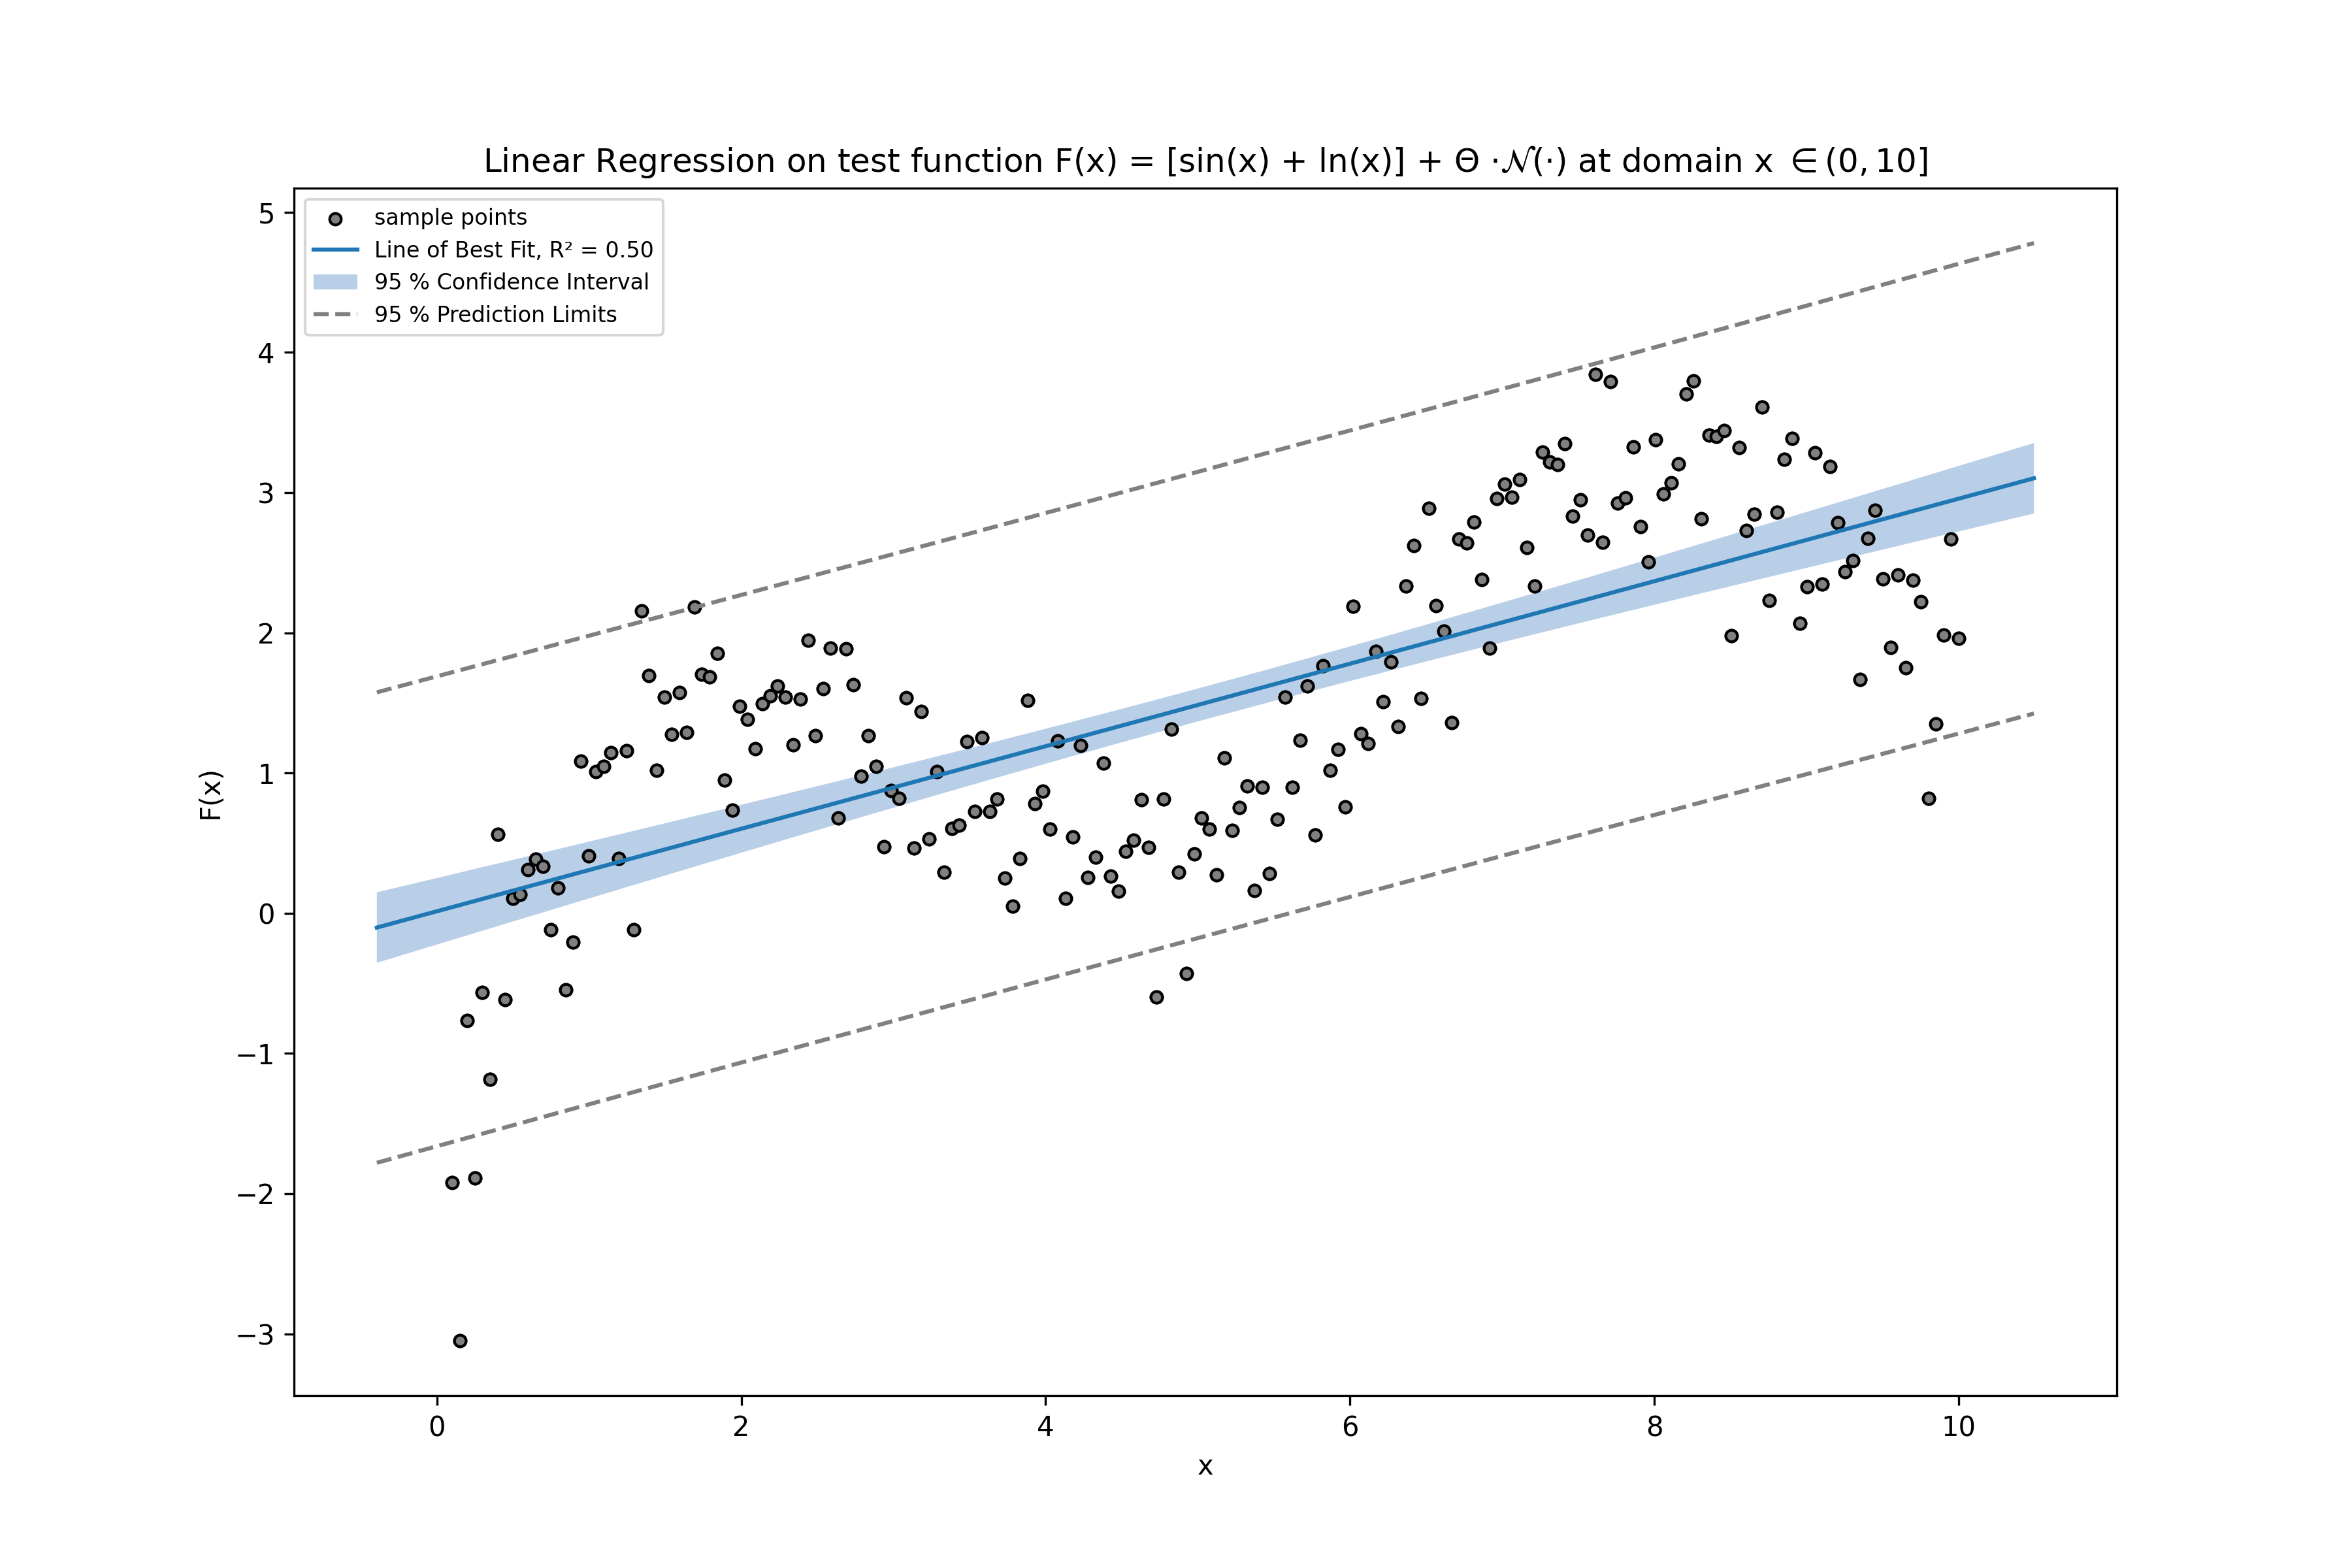
\includegraphics[width=1\textwidth,trim={0 0 0 0},clip]{figures/linear_regression.png}
    \caption[Linear Regression of the test function]{Linear Regression of the test function $F(x)$ with applied chi-square test and resulting 95\% confidence interval and 95 \% prediction limits}
    \label{fig: linear_regression_testfunction}    
\end{figure}
By implementing a \textit{Gradient Boosting Framework} with \textit{Decision Trees} as Base Learners one could benefit of the dynamic additive modeling with the non-linear behaving base-learners.
Because we're dealing with a more or less ``continuous`` domain of our function a least-squares regression model will be implemented as stated in section [\ref{sec: regr_boosted_trees}]. The pseudo-code which was written in [Alg. \ref{alg: gb_ls_algo}] will be implemented with the appropriate decision tree design [Alg. \ref{alg: tree_growing_algo}]. The self-written code is available in the following \href{https://github.com/probabilis/bs_ml/tree/master/from_scratch}{Github repository}.
\begin{figure}[!htpb]
    \centering
    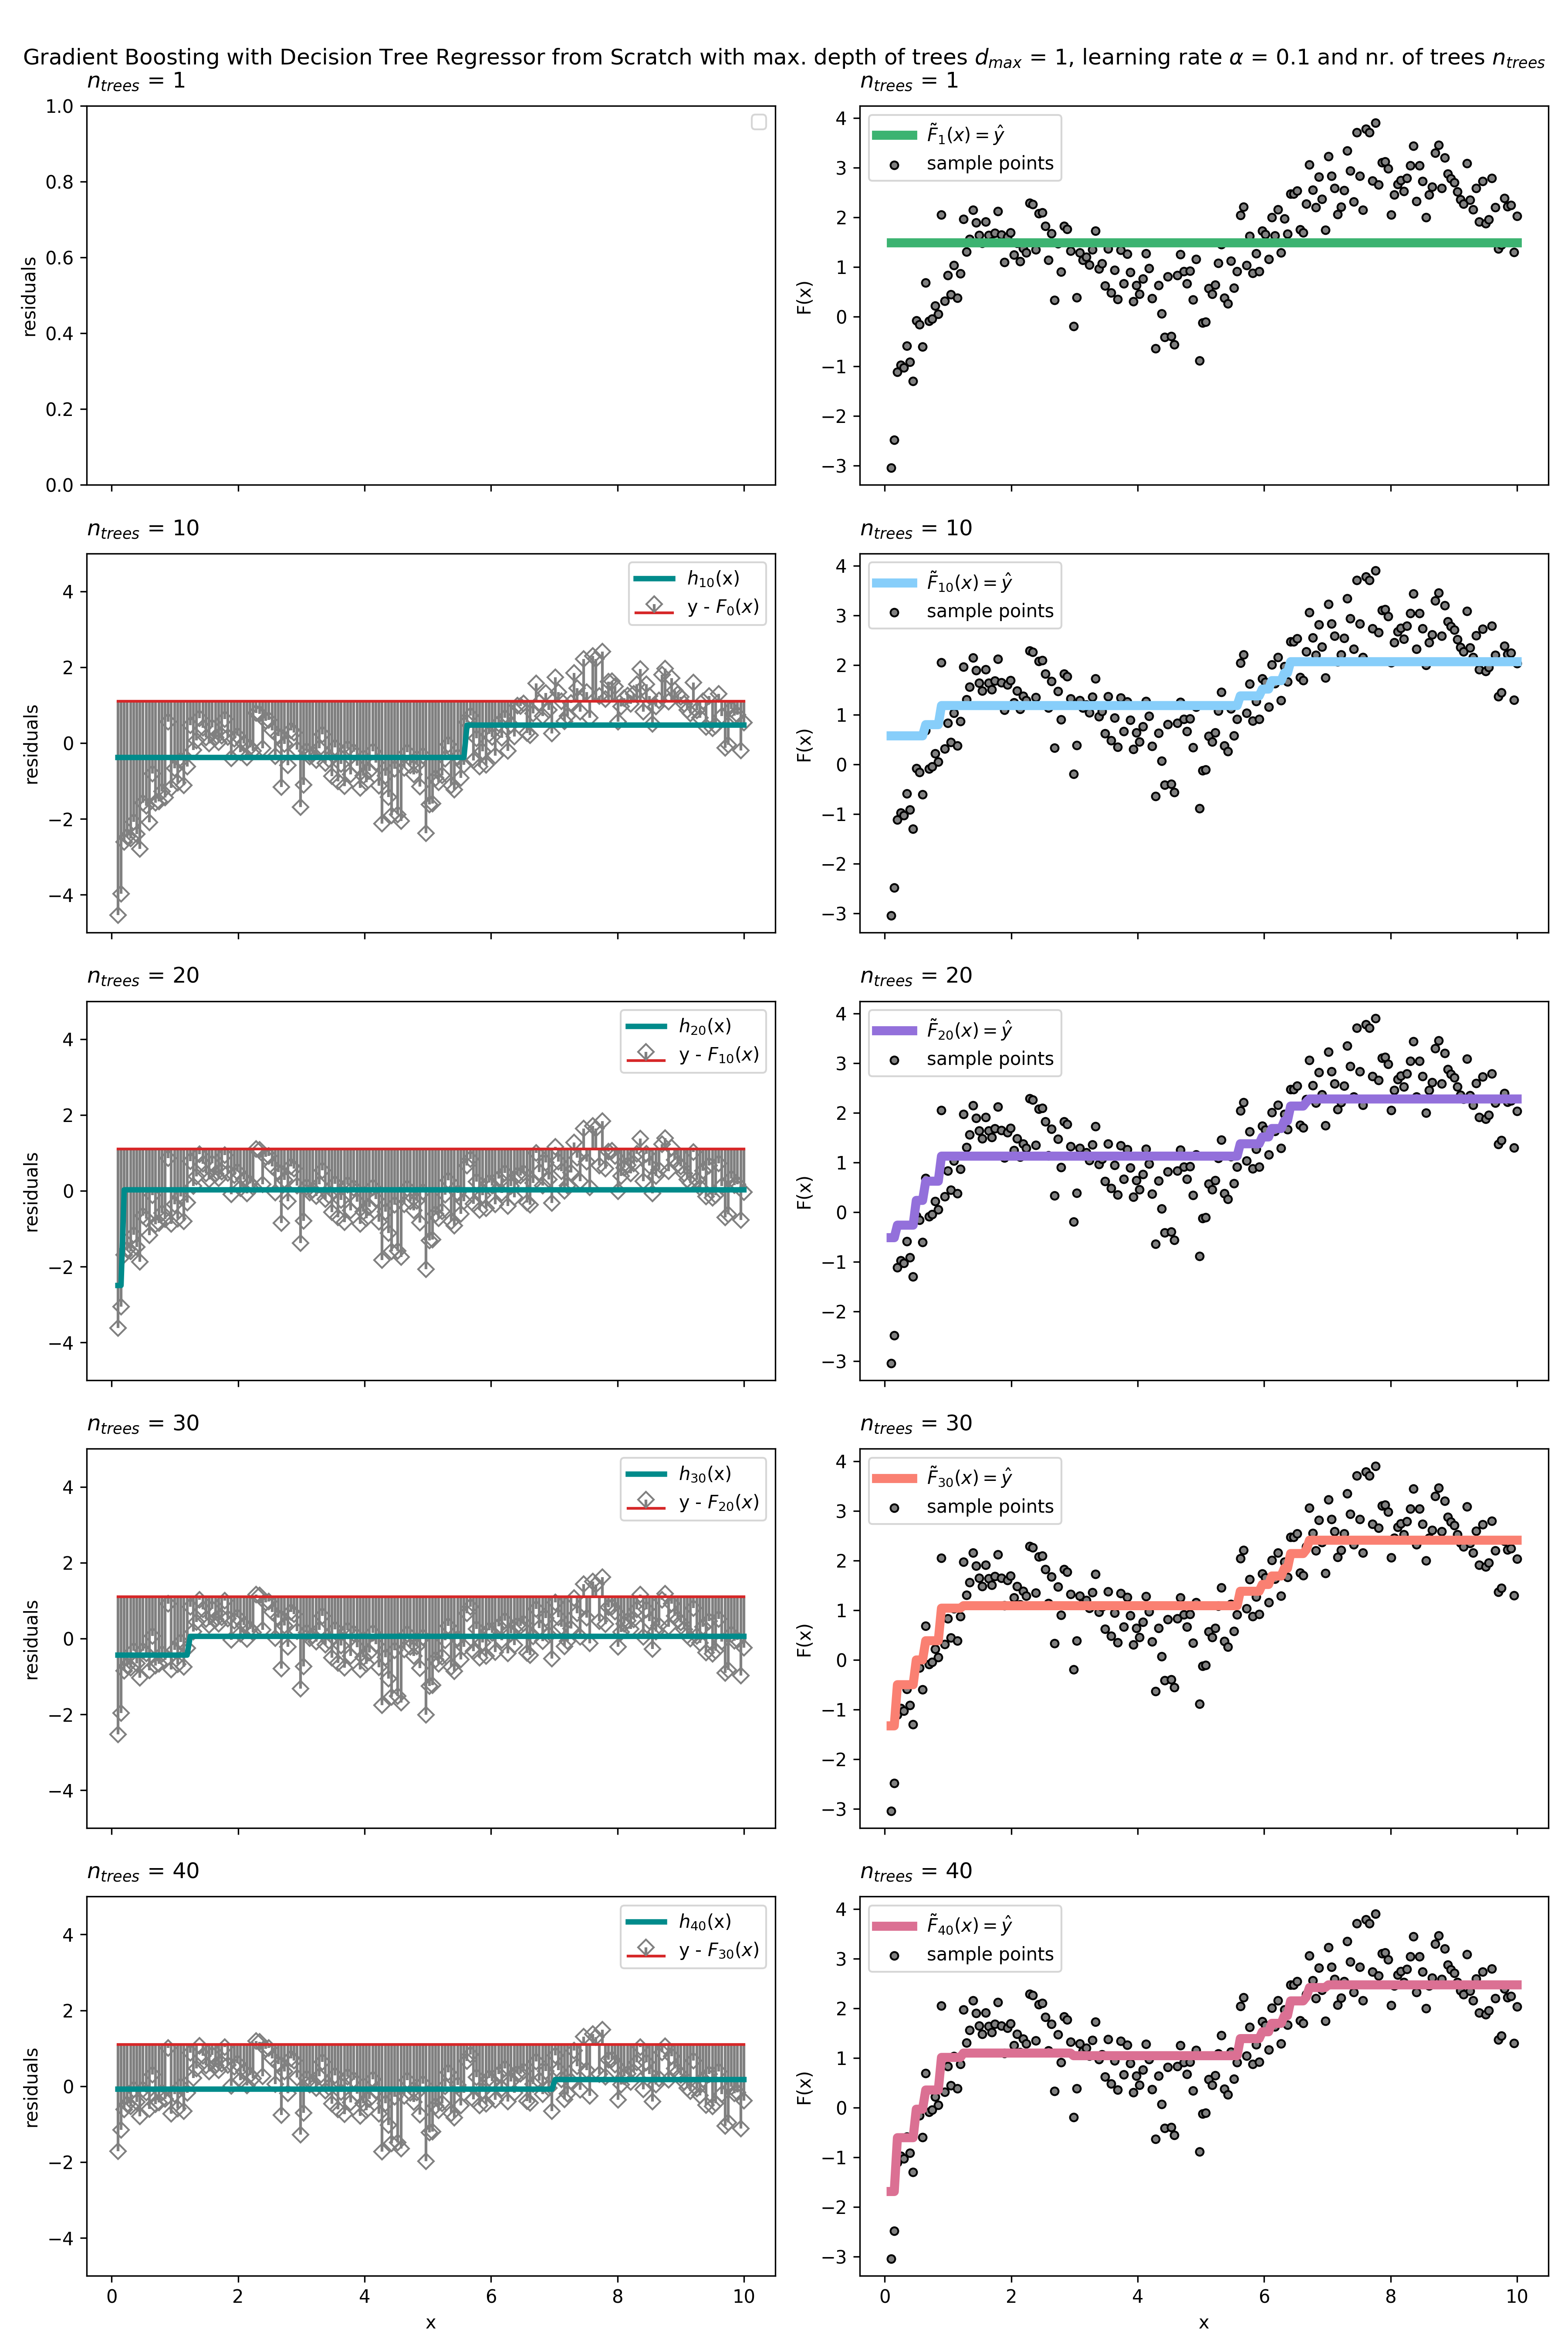
\includegraphics[width=0.95\textwidth,trim={0 0 0 0},clip]{figures/gbm_iterations.png}
    \caption[GBM framework iterations]{GBM framework with fixed depth of the decision tree regressor over iterations / left column shows the given residuals on each step and the generic function $h_m(x)$ which will be added to the model on each step / right column shows the sample points by the testfunction $F(x)$ and the predicted model $\tilde{F}_m(x) = \hat{y}$}
    \label{fig: gbm_iterations}    
\end{figure}
We can see that in the beginning the model will build the mean of the input space $x$ and adding the generic functions $h_m(x)$ on each step / iteration. This is equivalent by summing all different trees up, therefor $m = n_{trees}$. Because we've limited the model only to 40 estimators and even it's predicting the initial function quite well the full potential will be revealed within the right choice of hyperparameters.
%%%%%%%%%%%%%%%%%%%%%%%%%%%%%%%%%%%%%%%%%%%%%%%%%%%%%%%%%%%%%%%%%%%
\subsection{Gradient Boosting framework}
Comparing the mean squared error (MSE) shorthanded as deviance $\Delta$ over the boosting iterations (total number of different added trees). For the gradient boosting machine from scratch we'll use the last deviance over the total amount of estimators. We'll use the same test-function $F(x)$ as one dimensional regression problem.
We can obtain that the convergence of the prediction of the trained GB models with $n_{trees} = 100$ and $d_{max}$ = 1 over the given sample points are nearly identical with values of $\Delta_{SKLEARN/SKRATCH} \approx 0,208$  (depending on the random noise $\mathcal{N}(\cdot)$) with an deviation of $10^{-7}$ between both models.
\begin{figure}[!htpb]
    \centering
    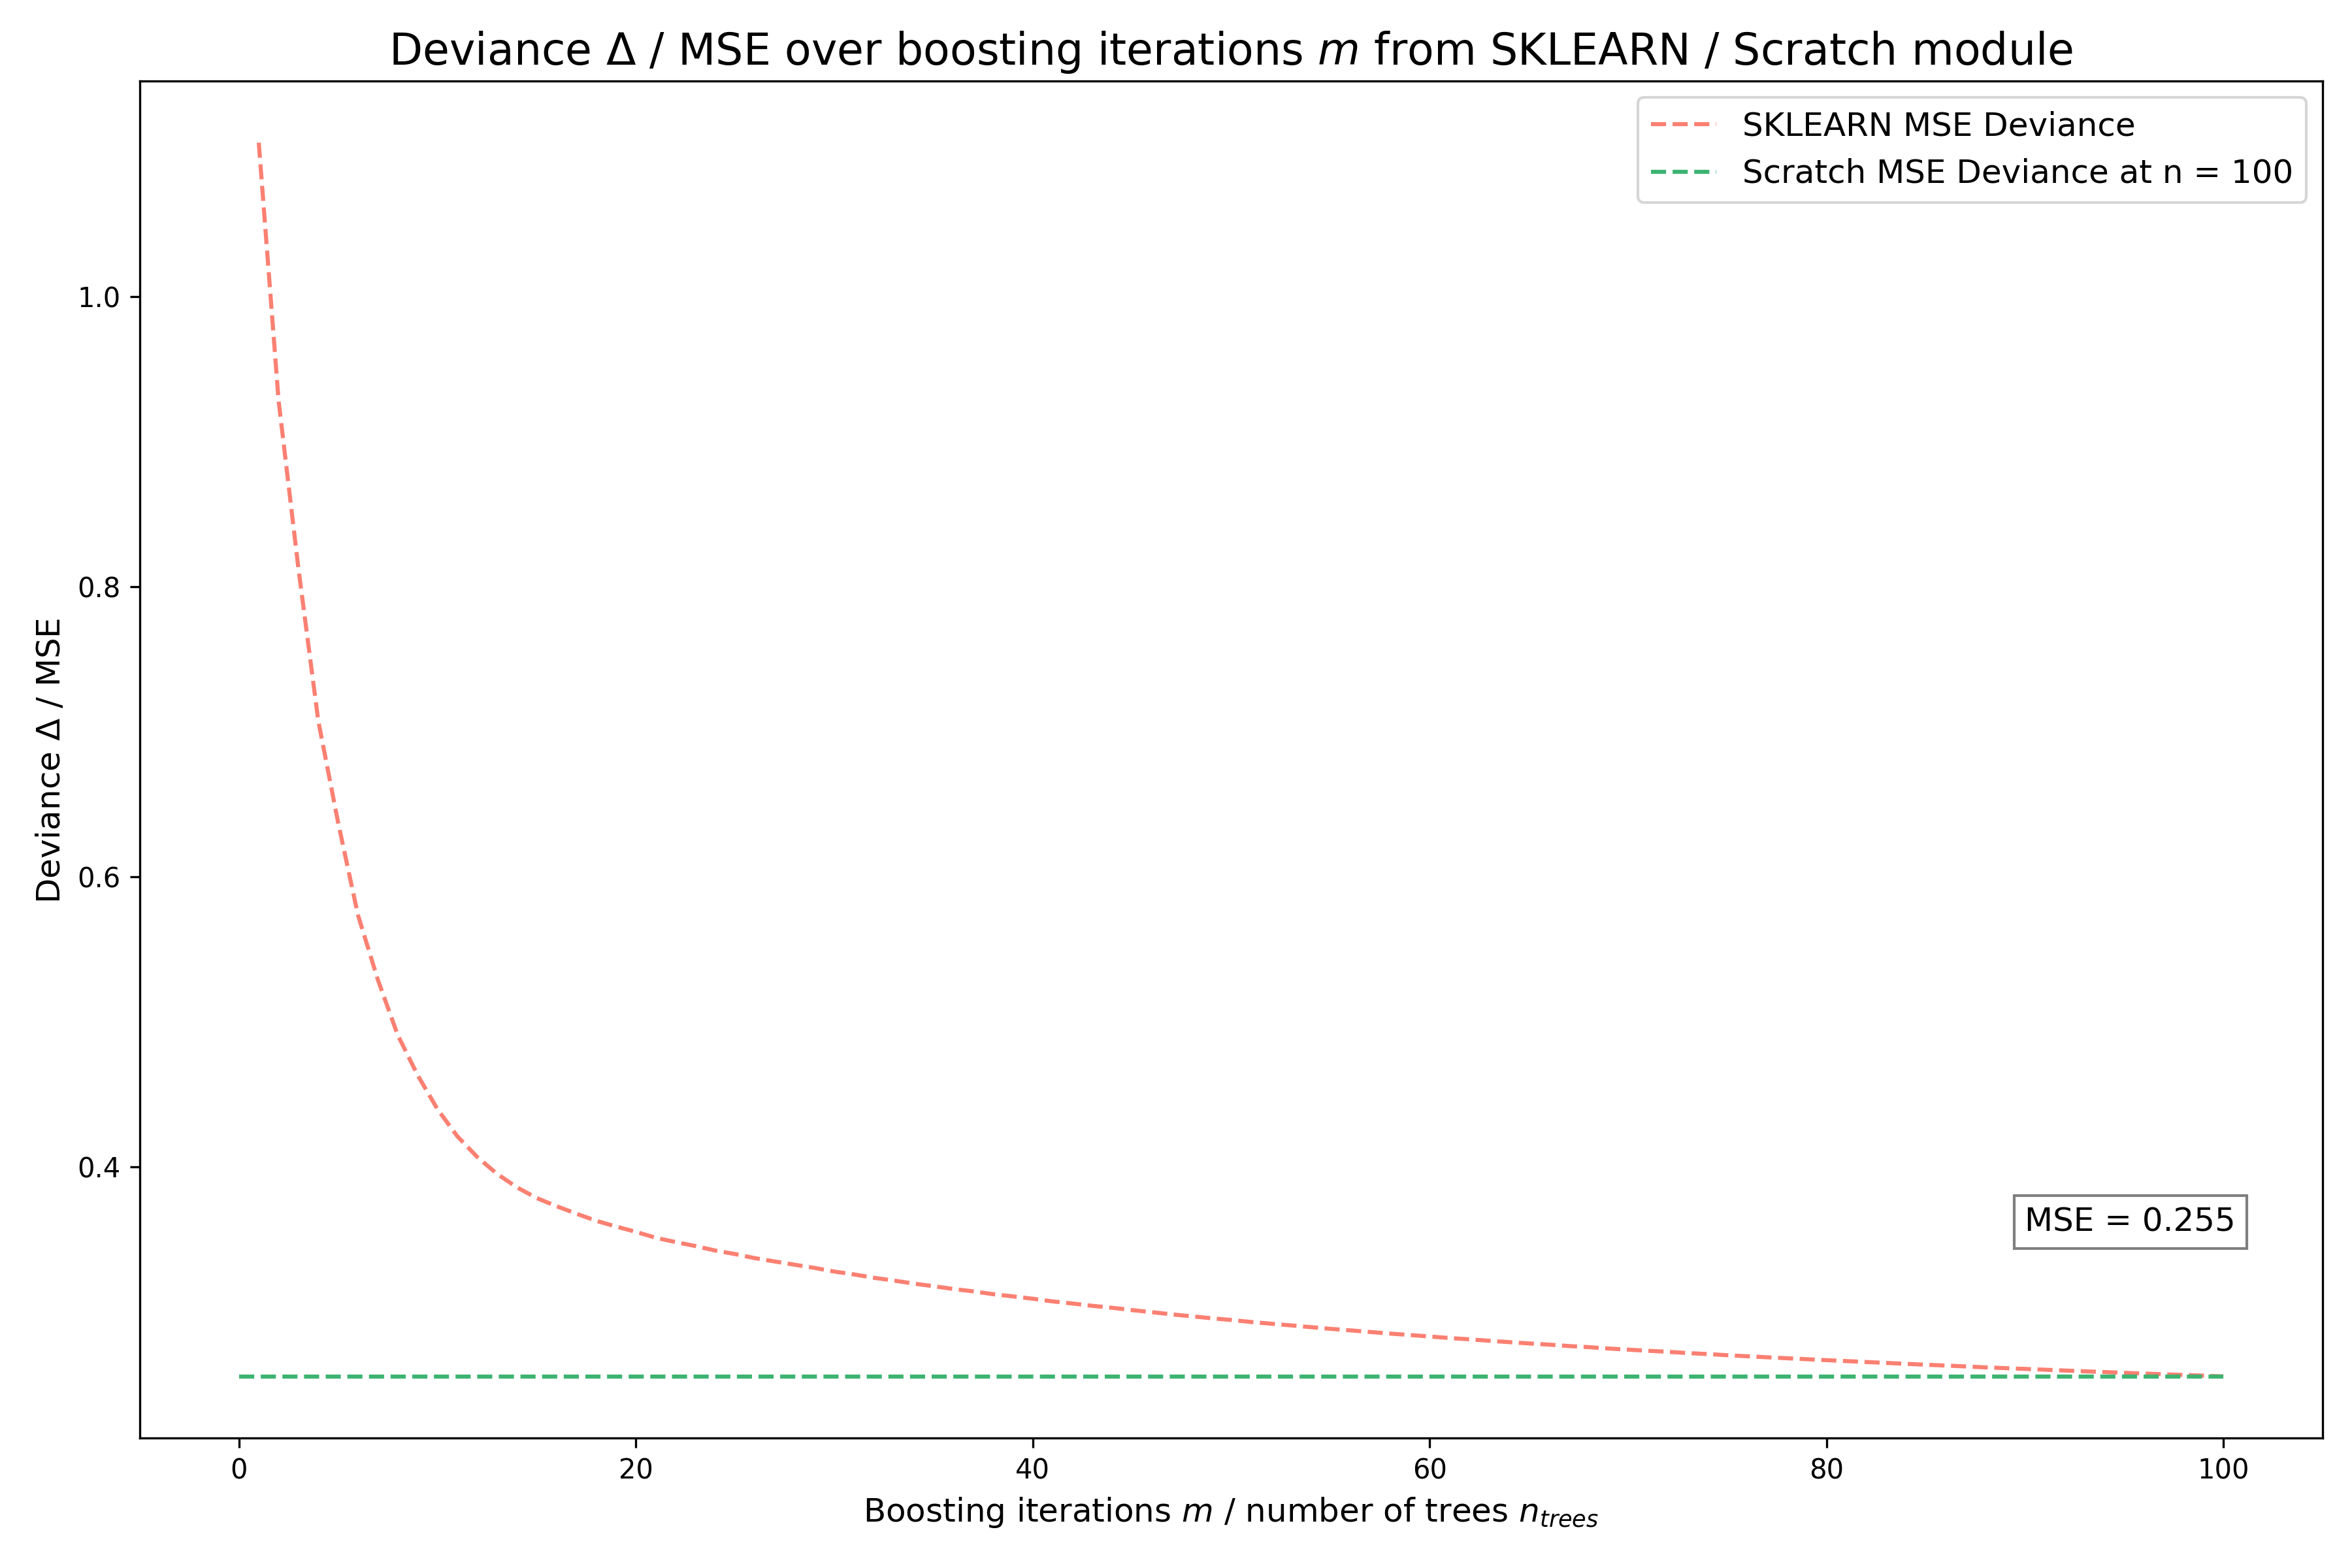
\includegraphics[width=1\textwidth,trim={0 0 0 0},clip]{figures/gbm_scratch_sklearn_loss_comparison.png}
    \caption[GBM framework comparison]{GBM framework comparison with fixed hyperparameters / from scratch with SKLEARN}
    \label{fig: gbm_comparison}    
\end{figure}
%%%%%%%%%%%%%%%%%%%%%%%%%%%%%%%%%%%%%%%%%%%%%%%%%%%%%%%%%%%%%%%%%%%
\subsection{Decision Tree Regressor framework}
Suppose we would not use additive modeling for predicting the test-function $F(x)$ but rather using only the decision tree regressor for splitting the input domain. This would result in the same solution as using only one estimator ($m$ = 1). \\ 
Therefor we could determine the best splitting point through calculating the mean square error on each sub-room of the inputs features as stated in section [\ref{sec: decision_trees}]. One could argue that using only one splitting function would give a solid approximation over the given sample points. Doing this for a maximal tree depth of $d_{max} = 1$ gives the following approximation $\tilde{y}$ of one estimator ($m = 1$) or multiple estimators ($m = 1000$) [Fig. \ref{fig: gbm_dt_comparison}]. 
\begin{figure}[!htpb]
    \centering
    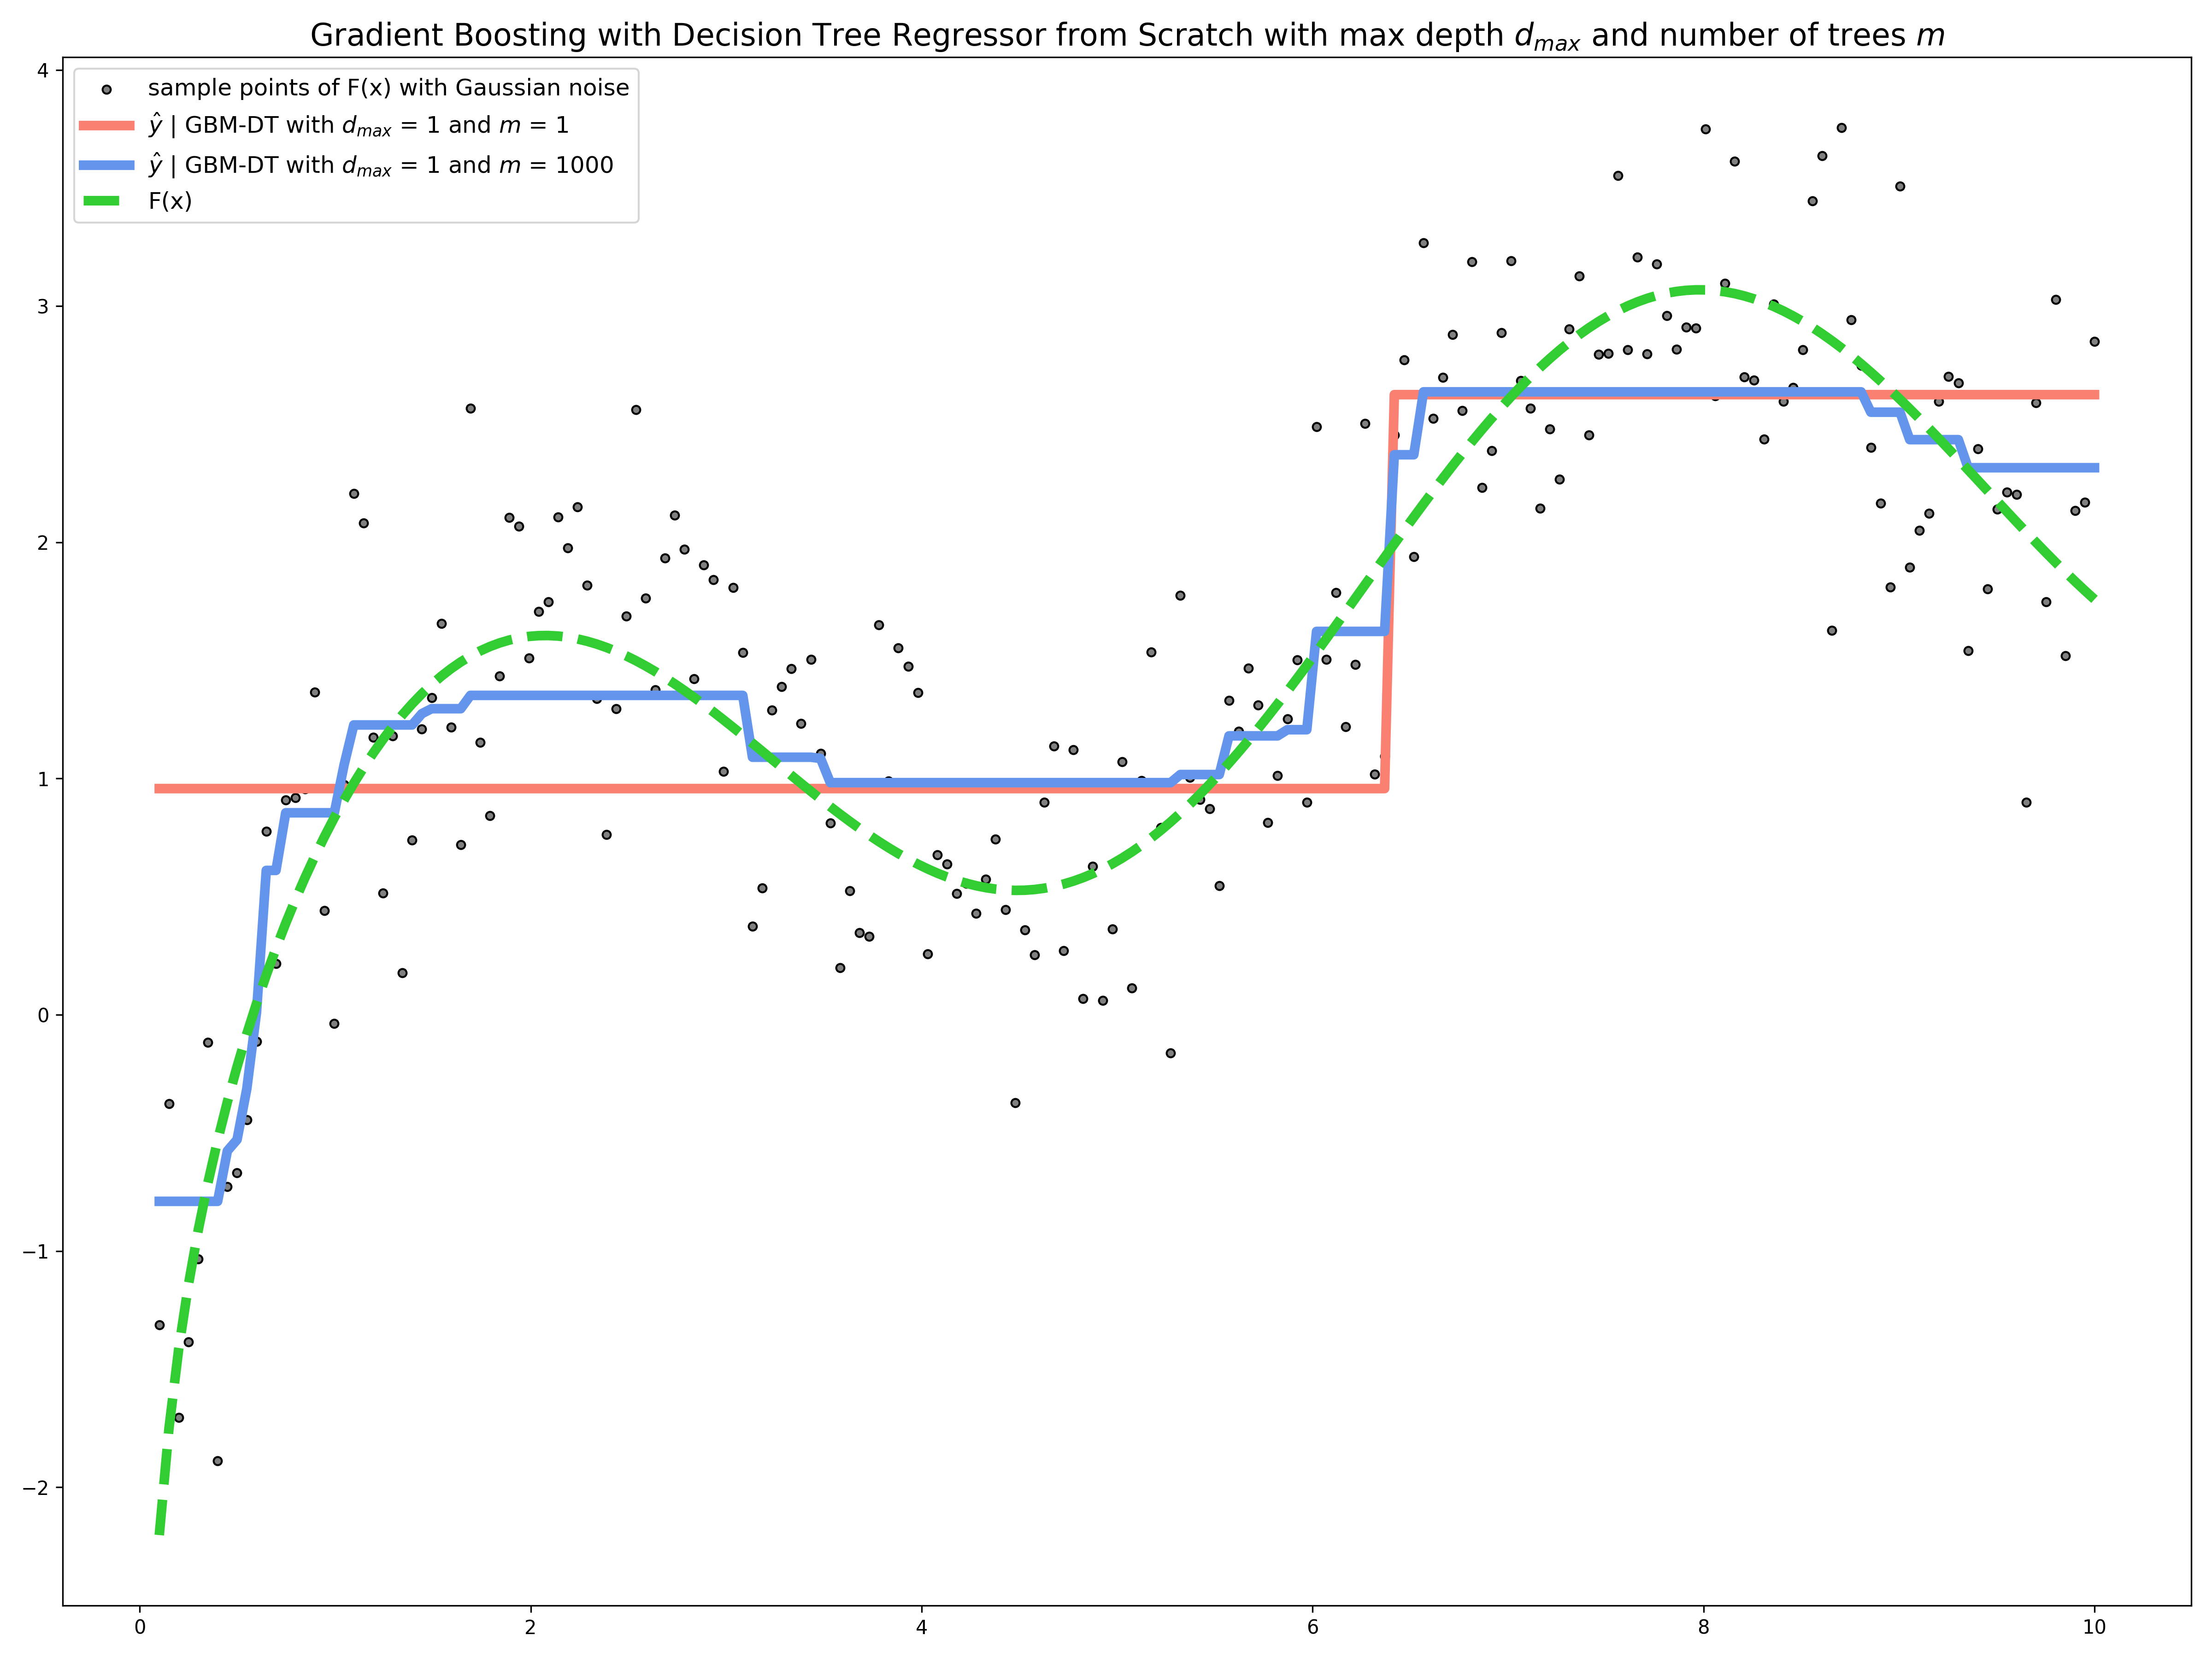
\includegraphics[width=1\textwidth,trim={0 0 0 0},clip]{figures/gbm_decision_tree_comparison.png}
    \caption[GBM-DT function prediction comparison over estimators]{GBM DT function prediction comparison for $m = 1$ or $m = 1000$ estimators (= number of trees $n_{trees}$)}
    \label{fig: gbm_dt_comparison}    
\end{figure}
\\
Here it's identifiable that the key advantage comes definitely within the additive modeling schematic. The decision tree regressor brings non-linearity whereby the number of estimators brings contour which characterizes this specific ensemble technique called boosting. \\
Taking a closer look in the decision tree splitting criteria over the test-function gives following approximations with tree structures $d_{max} \in \{1,2\}$ for the given data-set $x \in \mathcal{X}$ of the test function $F(x)$. When using a maximum depth of $d_{max} = 1$, so only one layer, would set the splitting criteria as shown in figure [\ref{fig: dt_comp_1} \& \ref{fig: dt_split_1}].
\begin{figure}[htbp]
\begin{minipage}[t]{7cm}
\vspace{0pt}
\centering
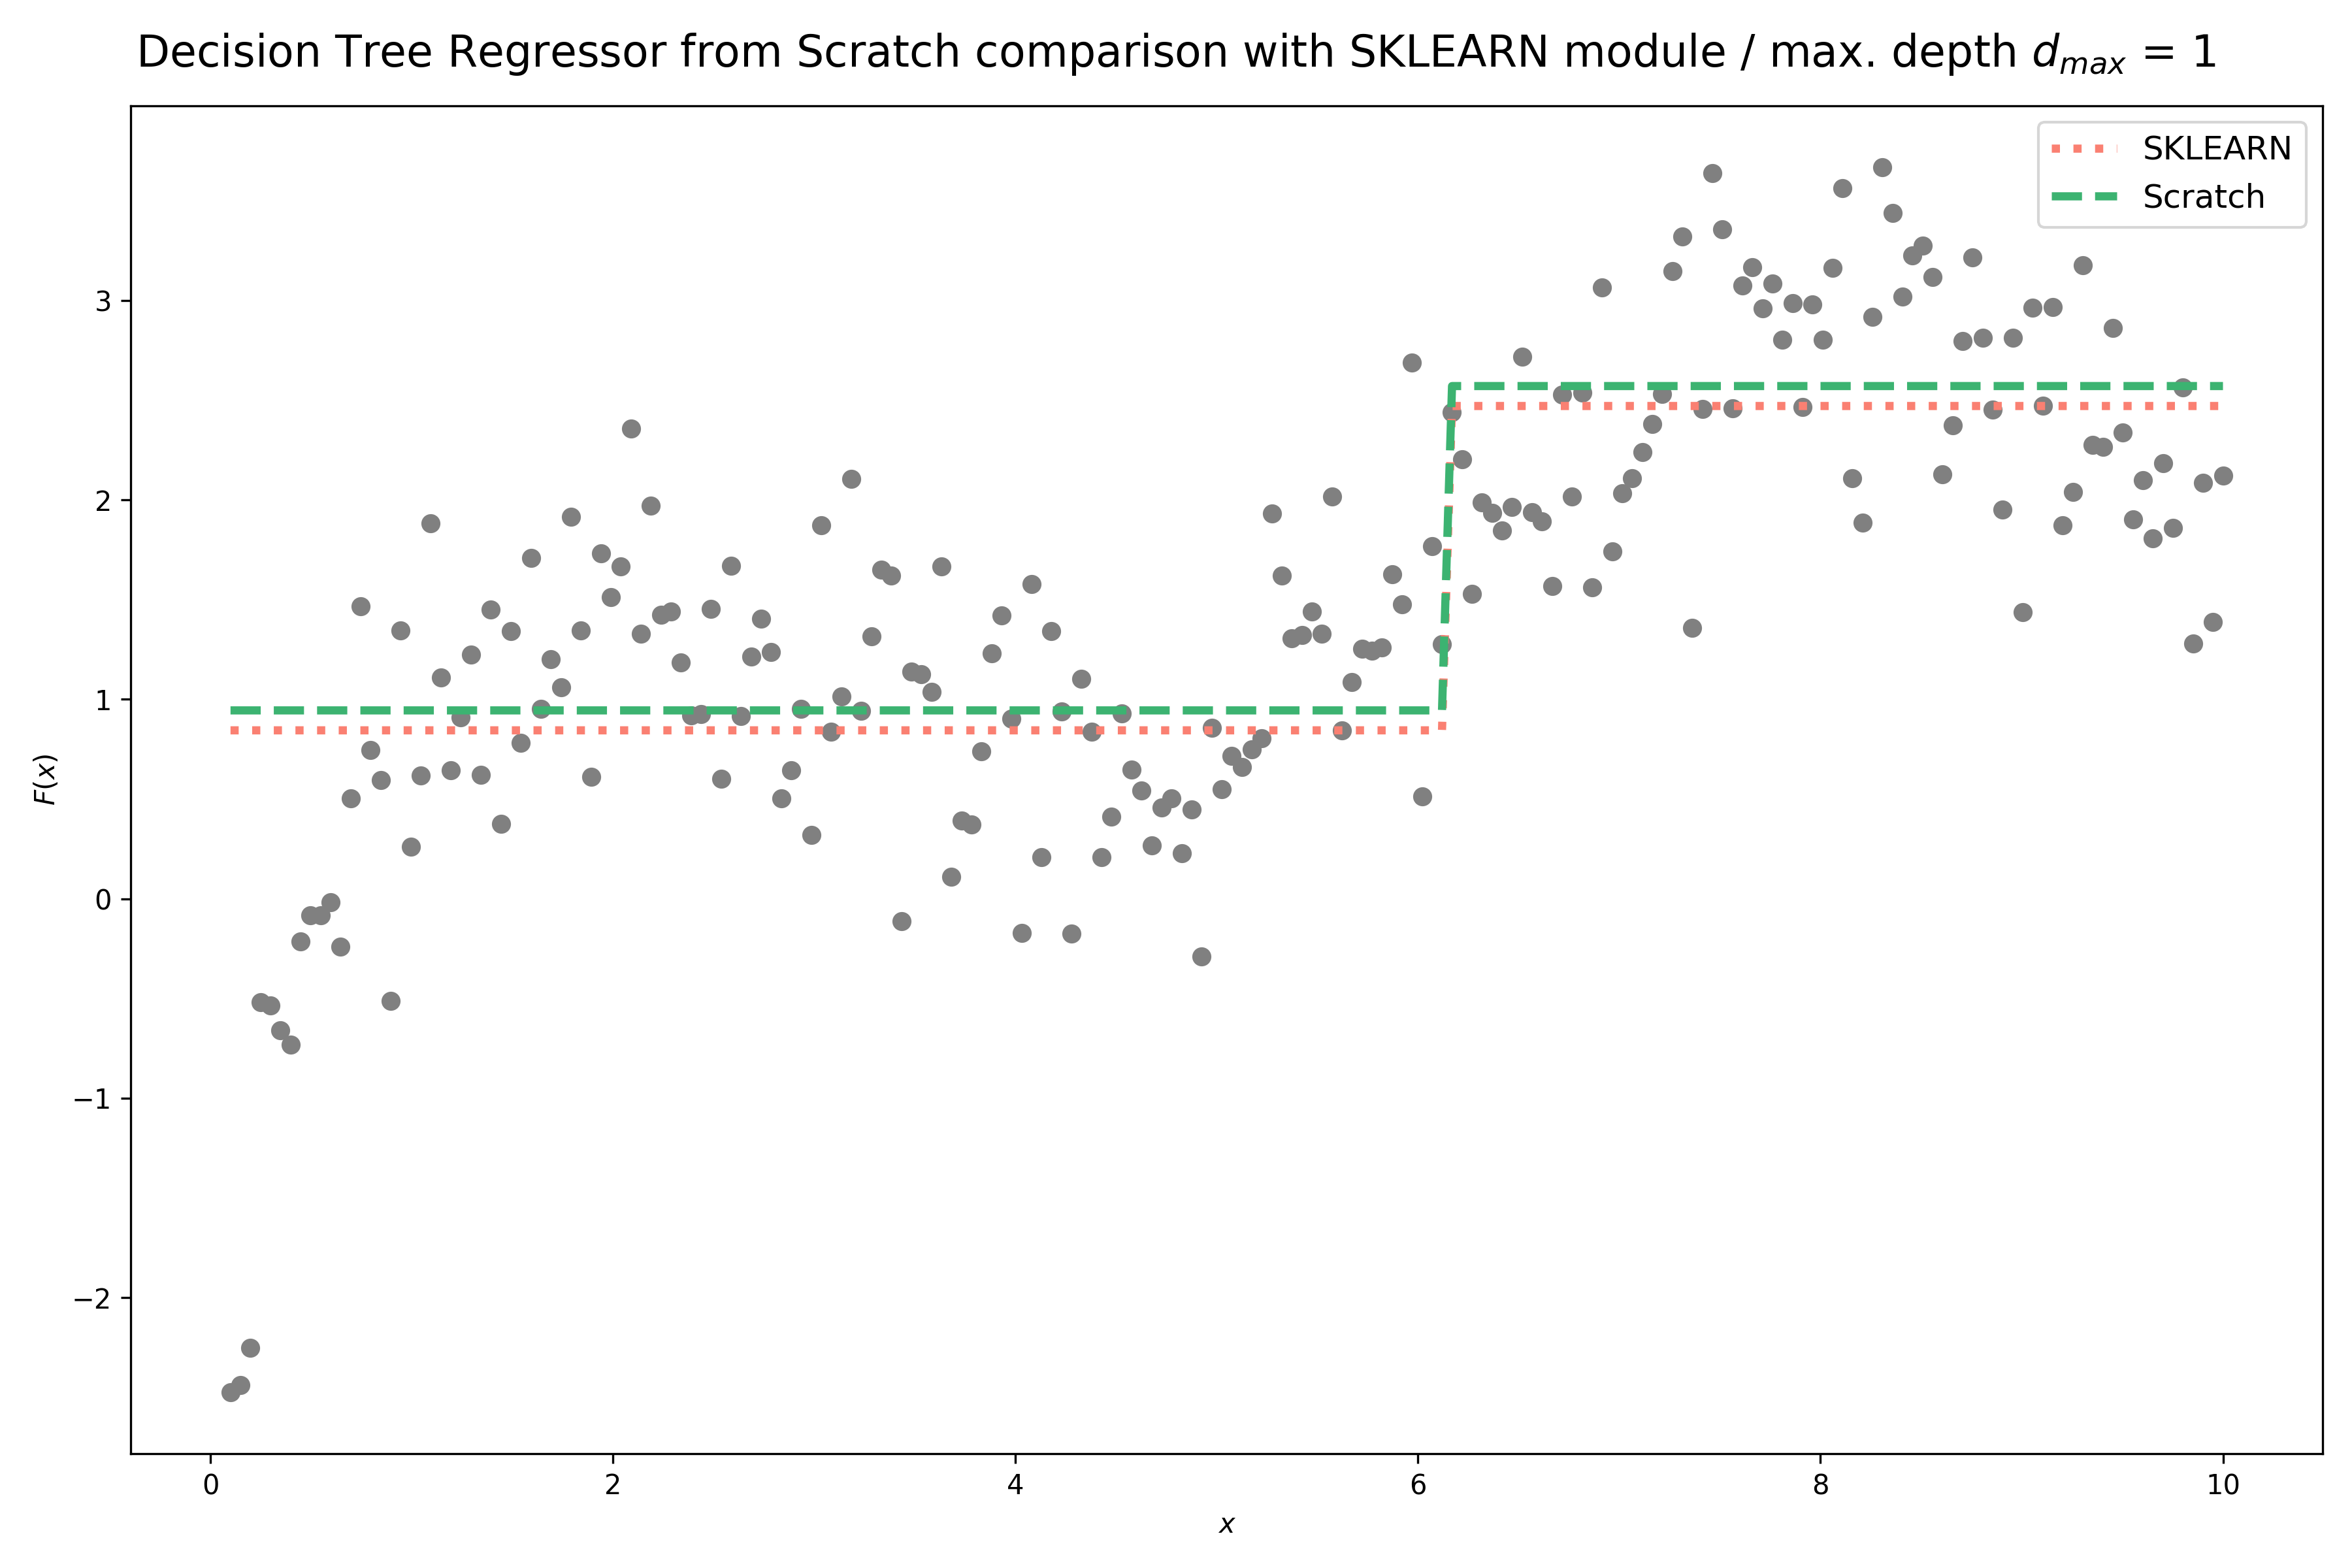
\includegraphics[width=1\textwidth,trim={0 0 0 0},clip]{figures/decision_tree_regressor_comparison_md=1.png}
\caption[Decision Tree Regressor / One Layer]{Decision Tree Regressor / Sample points and split. function / $d_{max} = 1$}
\label{fig: dt_comp_1}  
\end{minipage}
\hfill
\begin{minipage}[t]{6cm}
\vspace{0pt}
\centering
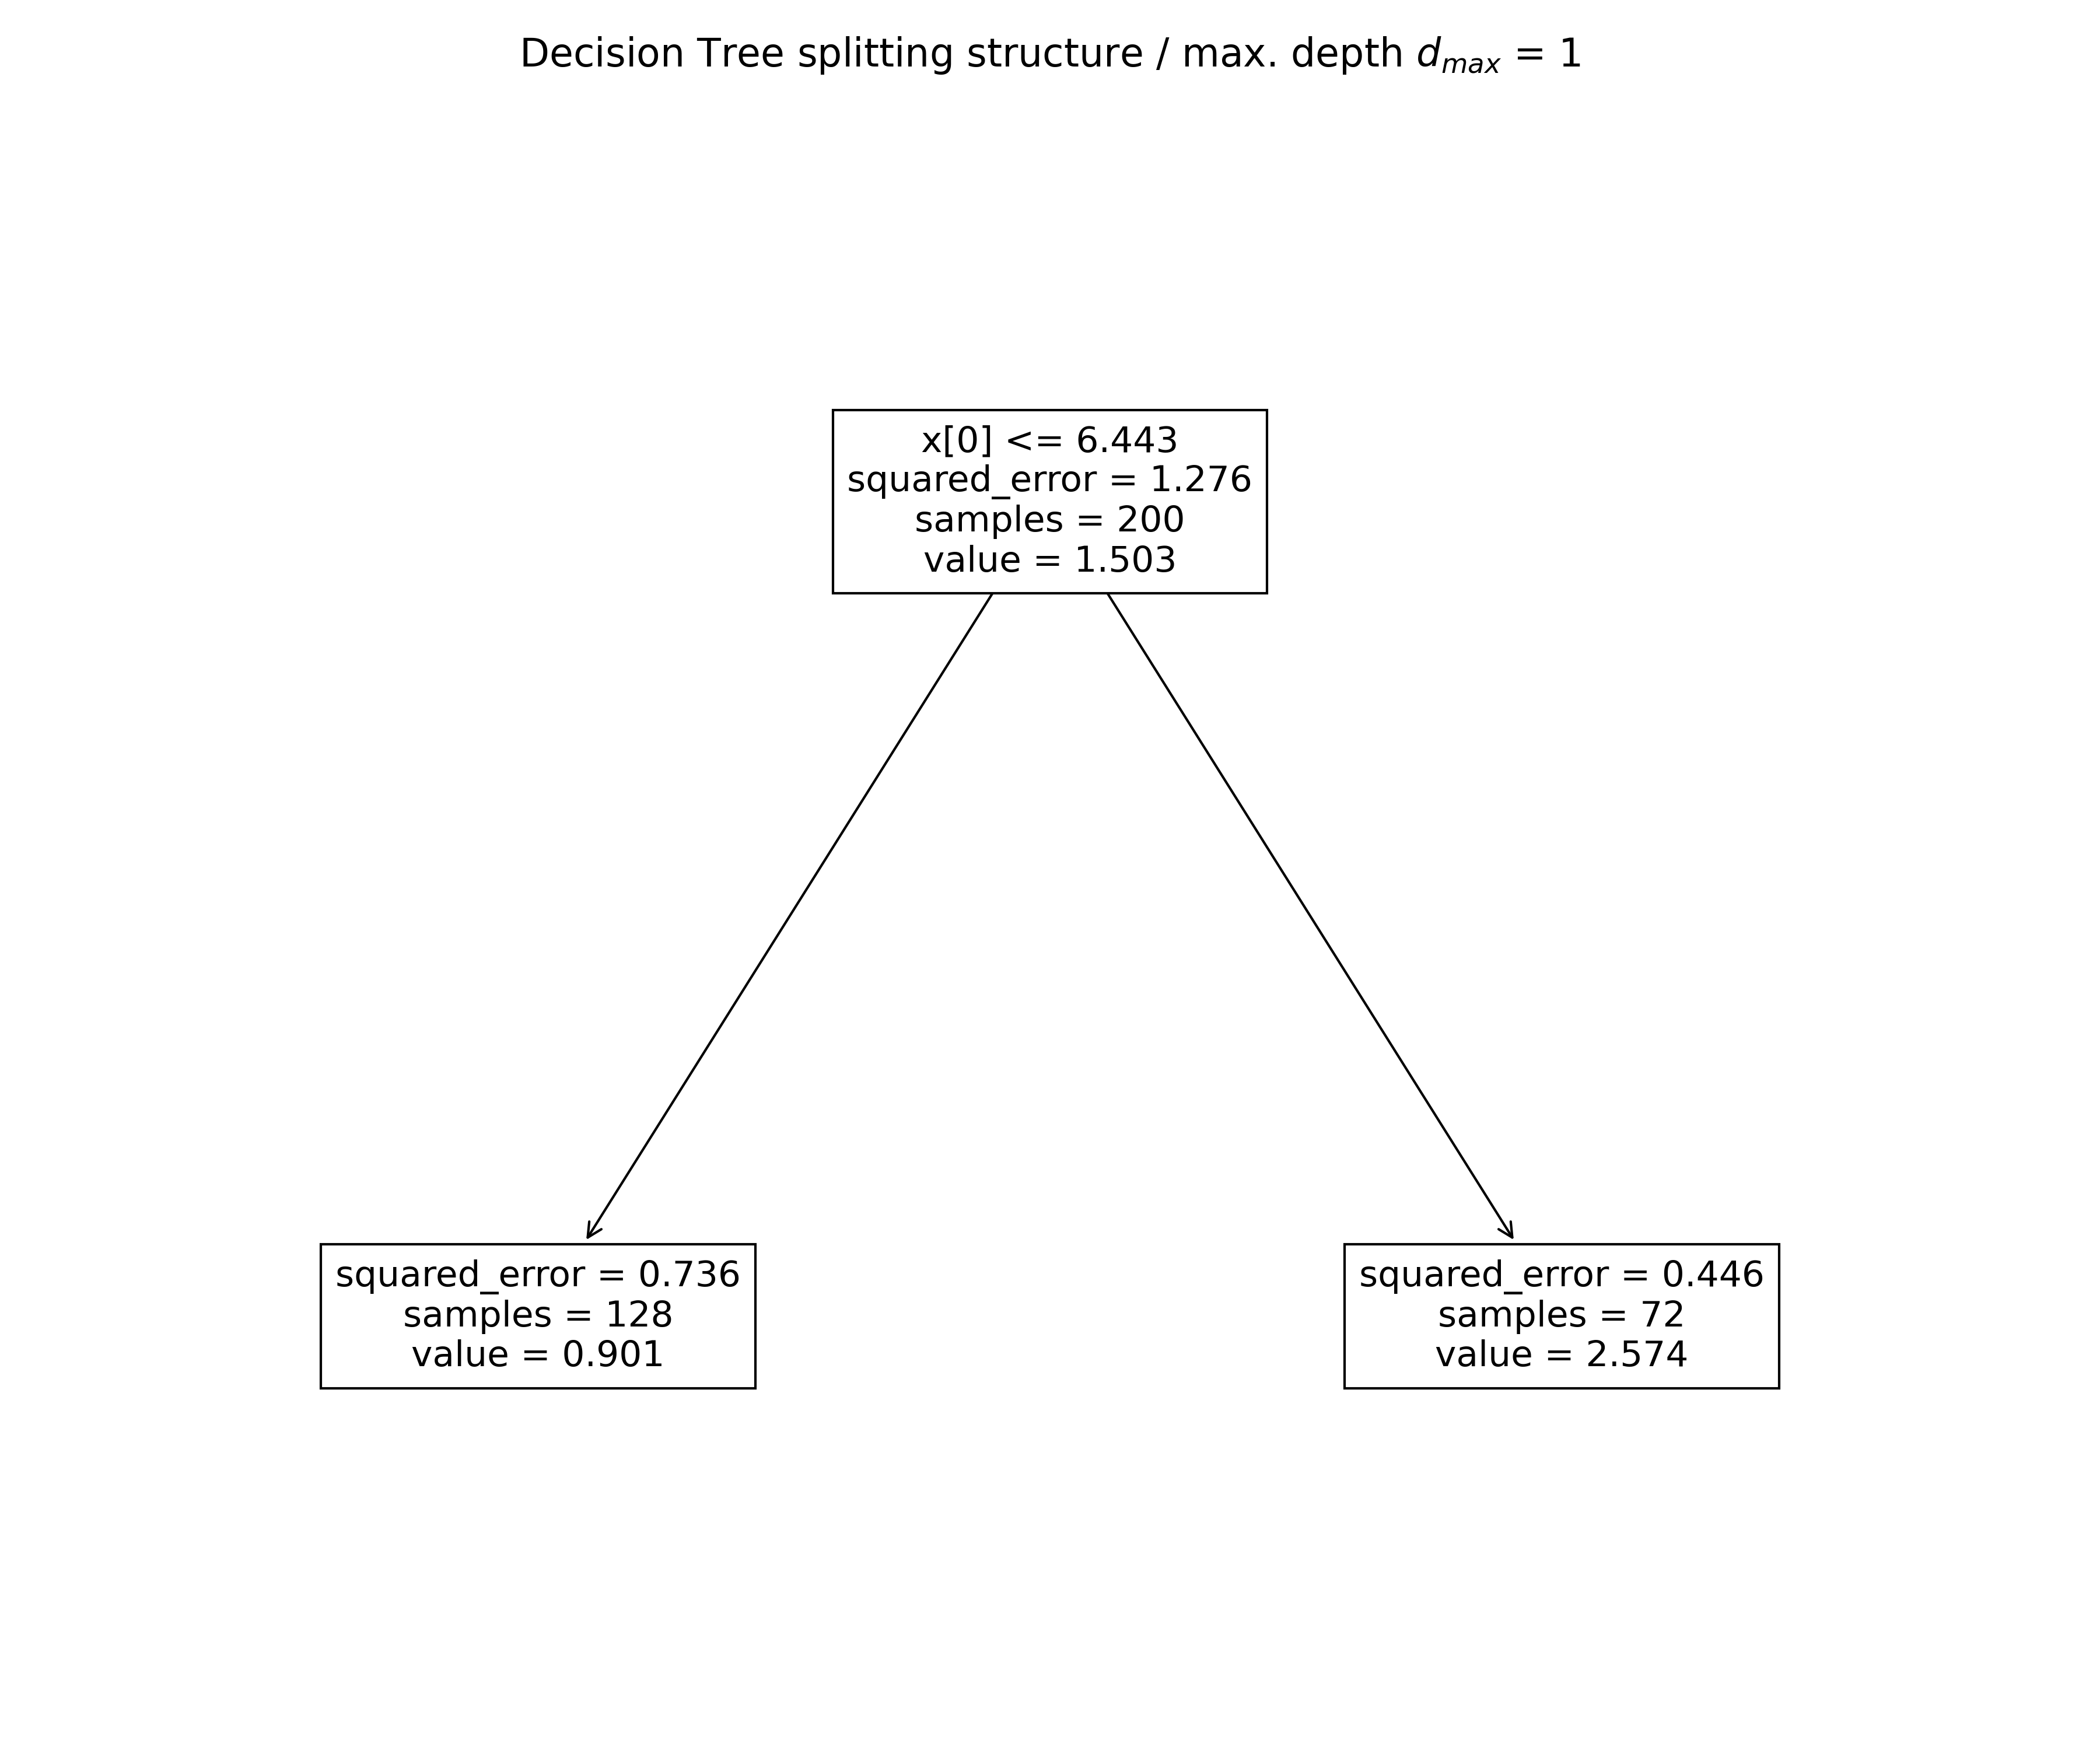
\includegraphics[width=1\textwidth,trim={0 0 0 0},clip]{figures/decision_tree_splitting_structure_md=1.png}
\caption[Decision Path / One Layer]{Decision Path / $d_{max} = 1$}
\label{fig: dt_split_1} 
\end{minipage}
\end{figure}
\\
If $x_i$ is smaller than a threshold then $\tilde{y}$ gets assigned the mean:
\begin{center}
    $x_i \lessapprox 6,44 \rightarrow \tilde{y} \approx 0,9$ (left branch) $\vee$ $x_i \gtrapprox 6,44 \rightarrow \tilde{y} \approx 2,58$ (right branch). 
\end{center}
This would result in 128 samples on the left and 72 sample on the right side given the data-set with an one layer tree structure with in total 2 leaves. \\
By increasing the depth of the tree to $d_{max} = 2$ one get a system with 4 leaves and 3 optimal splitting rules as shown in figure [\ref{fig: dt_comp_2} \& \ref{fig: dt_split_2}].
\begin{figure}[htbp]
\begin{minipage}[t]{7cm}
\vspace{0pt}
\centering
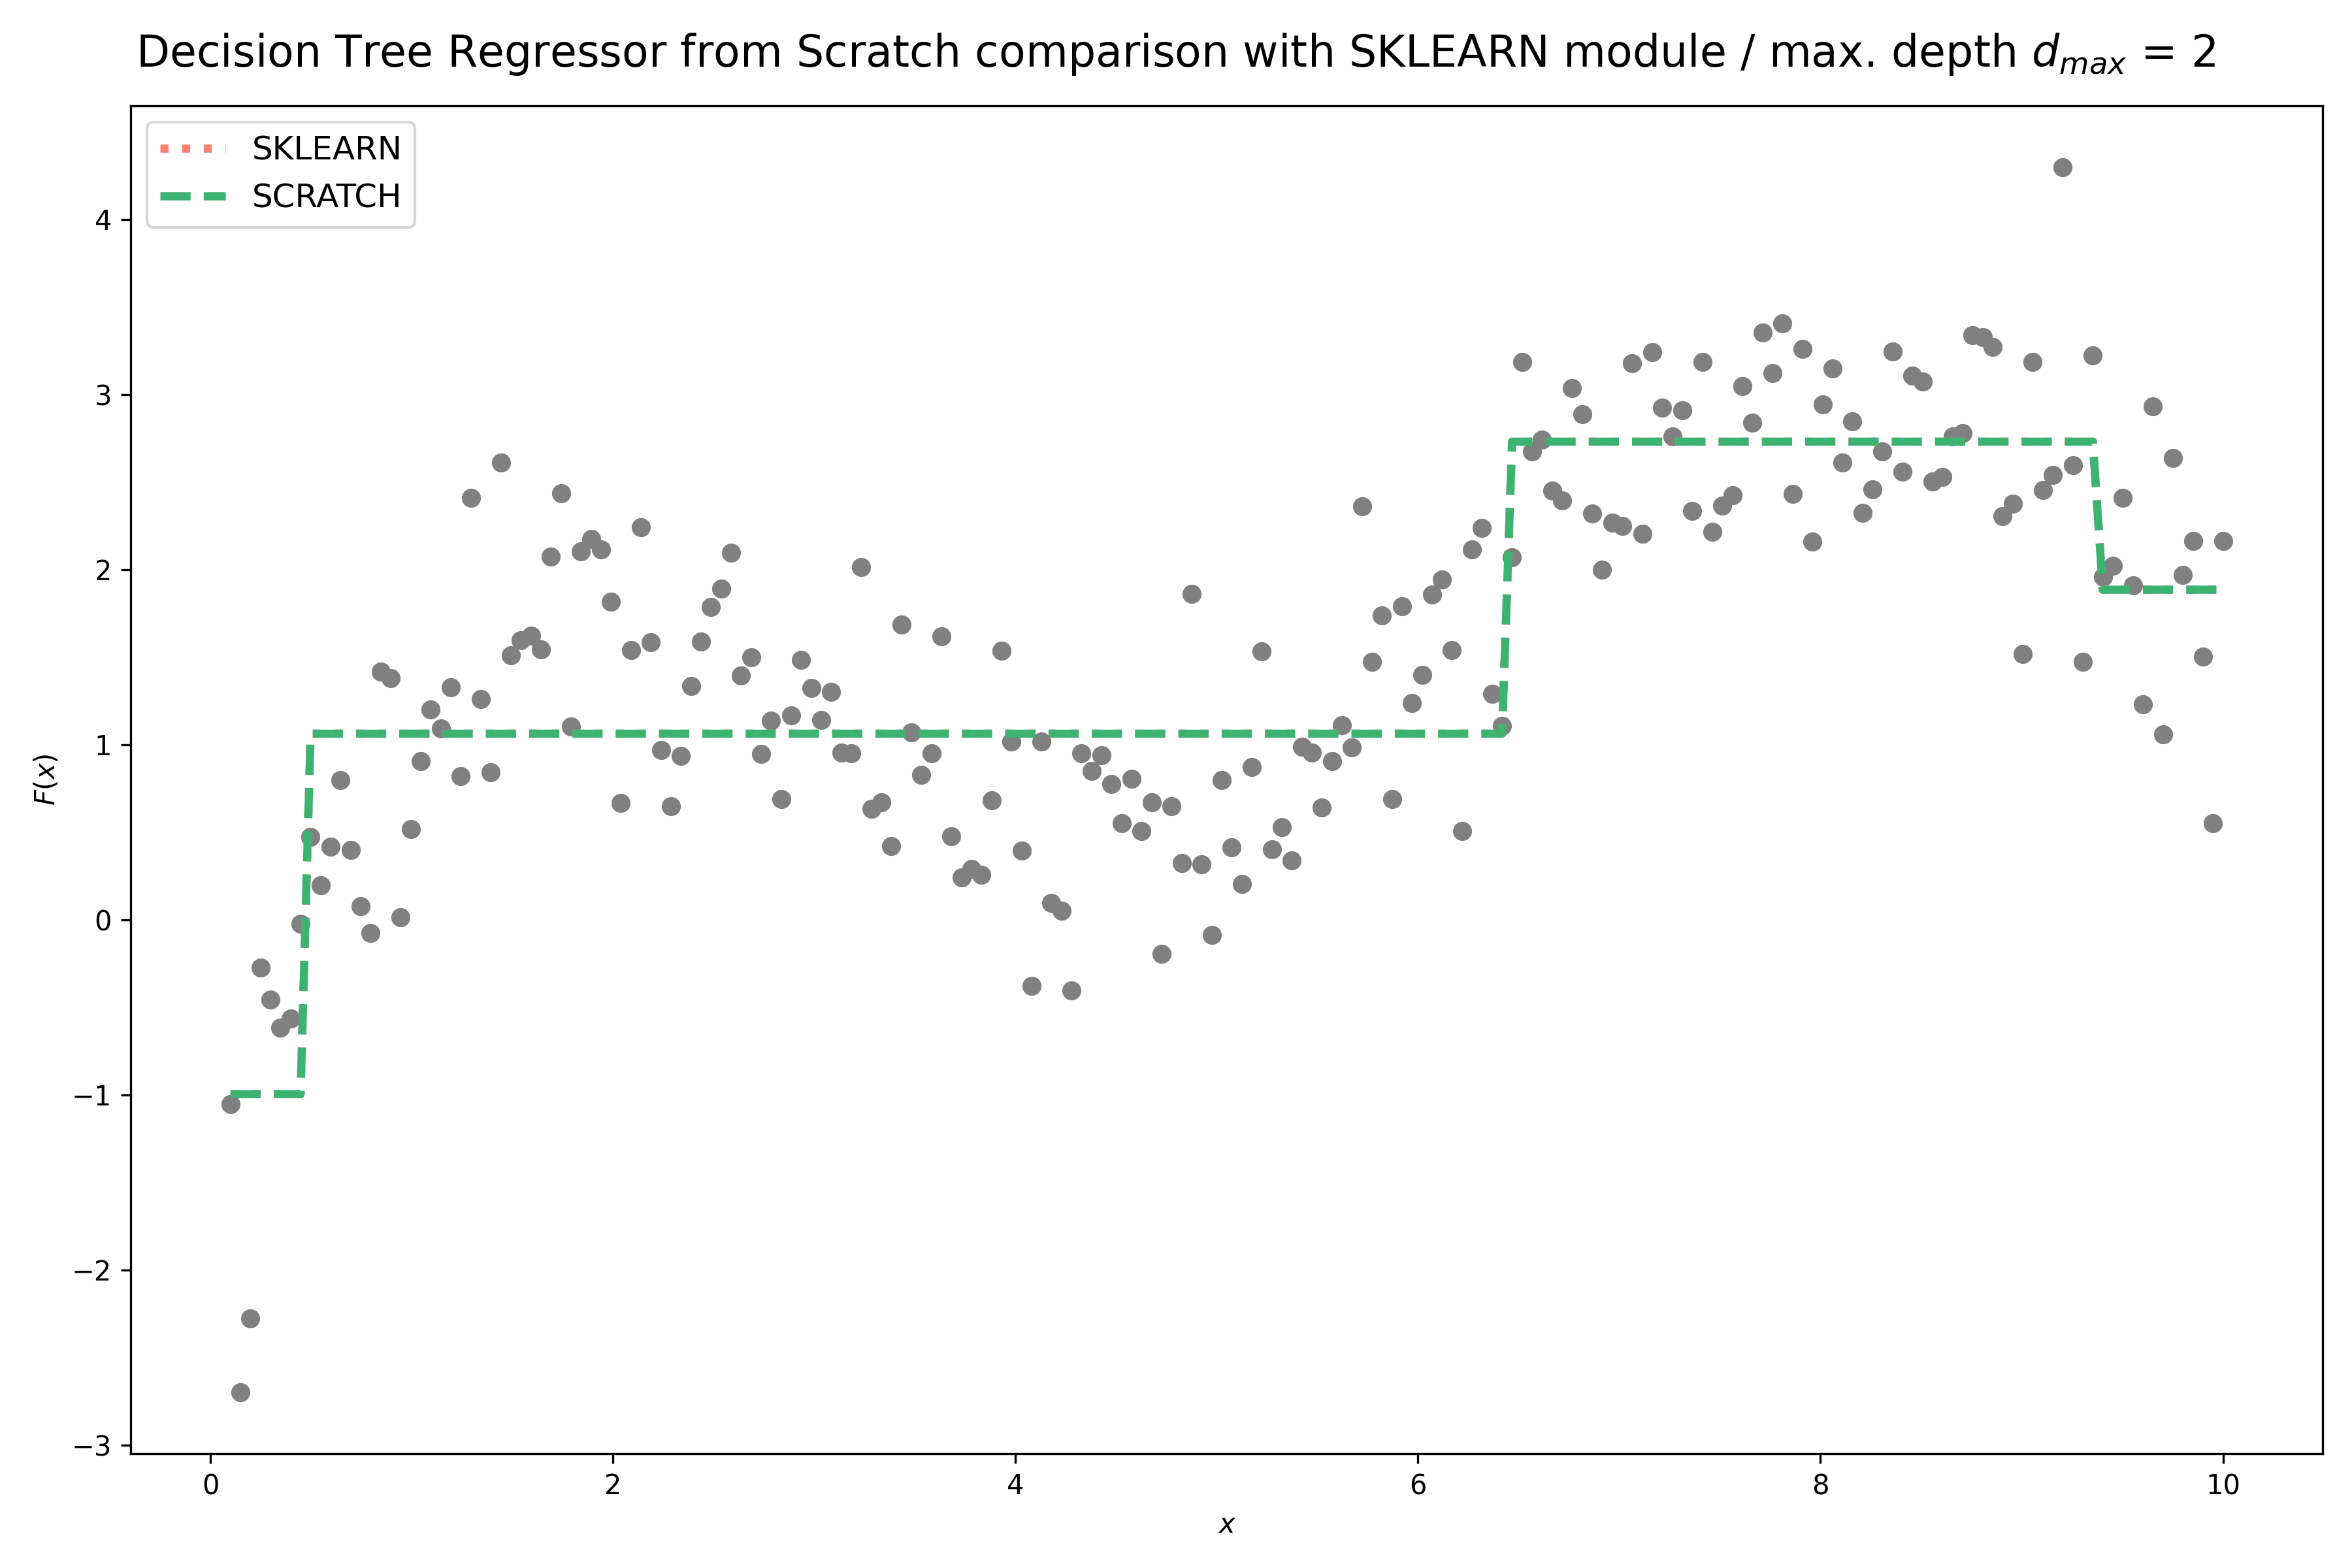
\includegraphics[width=1\textwidth,trim={0 0 0 0},clip]{figures/decision_tree_regressor_comparison_md=2.png}
\caption[Decision Tree Regressor / Two Layers]{Decision Tree Regressor / Sample points and split. function / $d_{max} = 2$}
\label{fig: dt_comp_2}  
\end{minipage}
\hfill
\begin{minipage}[t]{6cm}
\vspace{0pt}
\centering
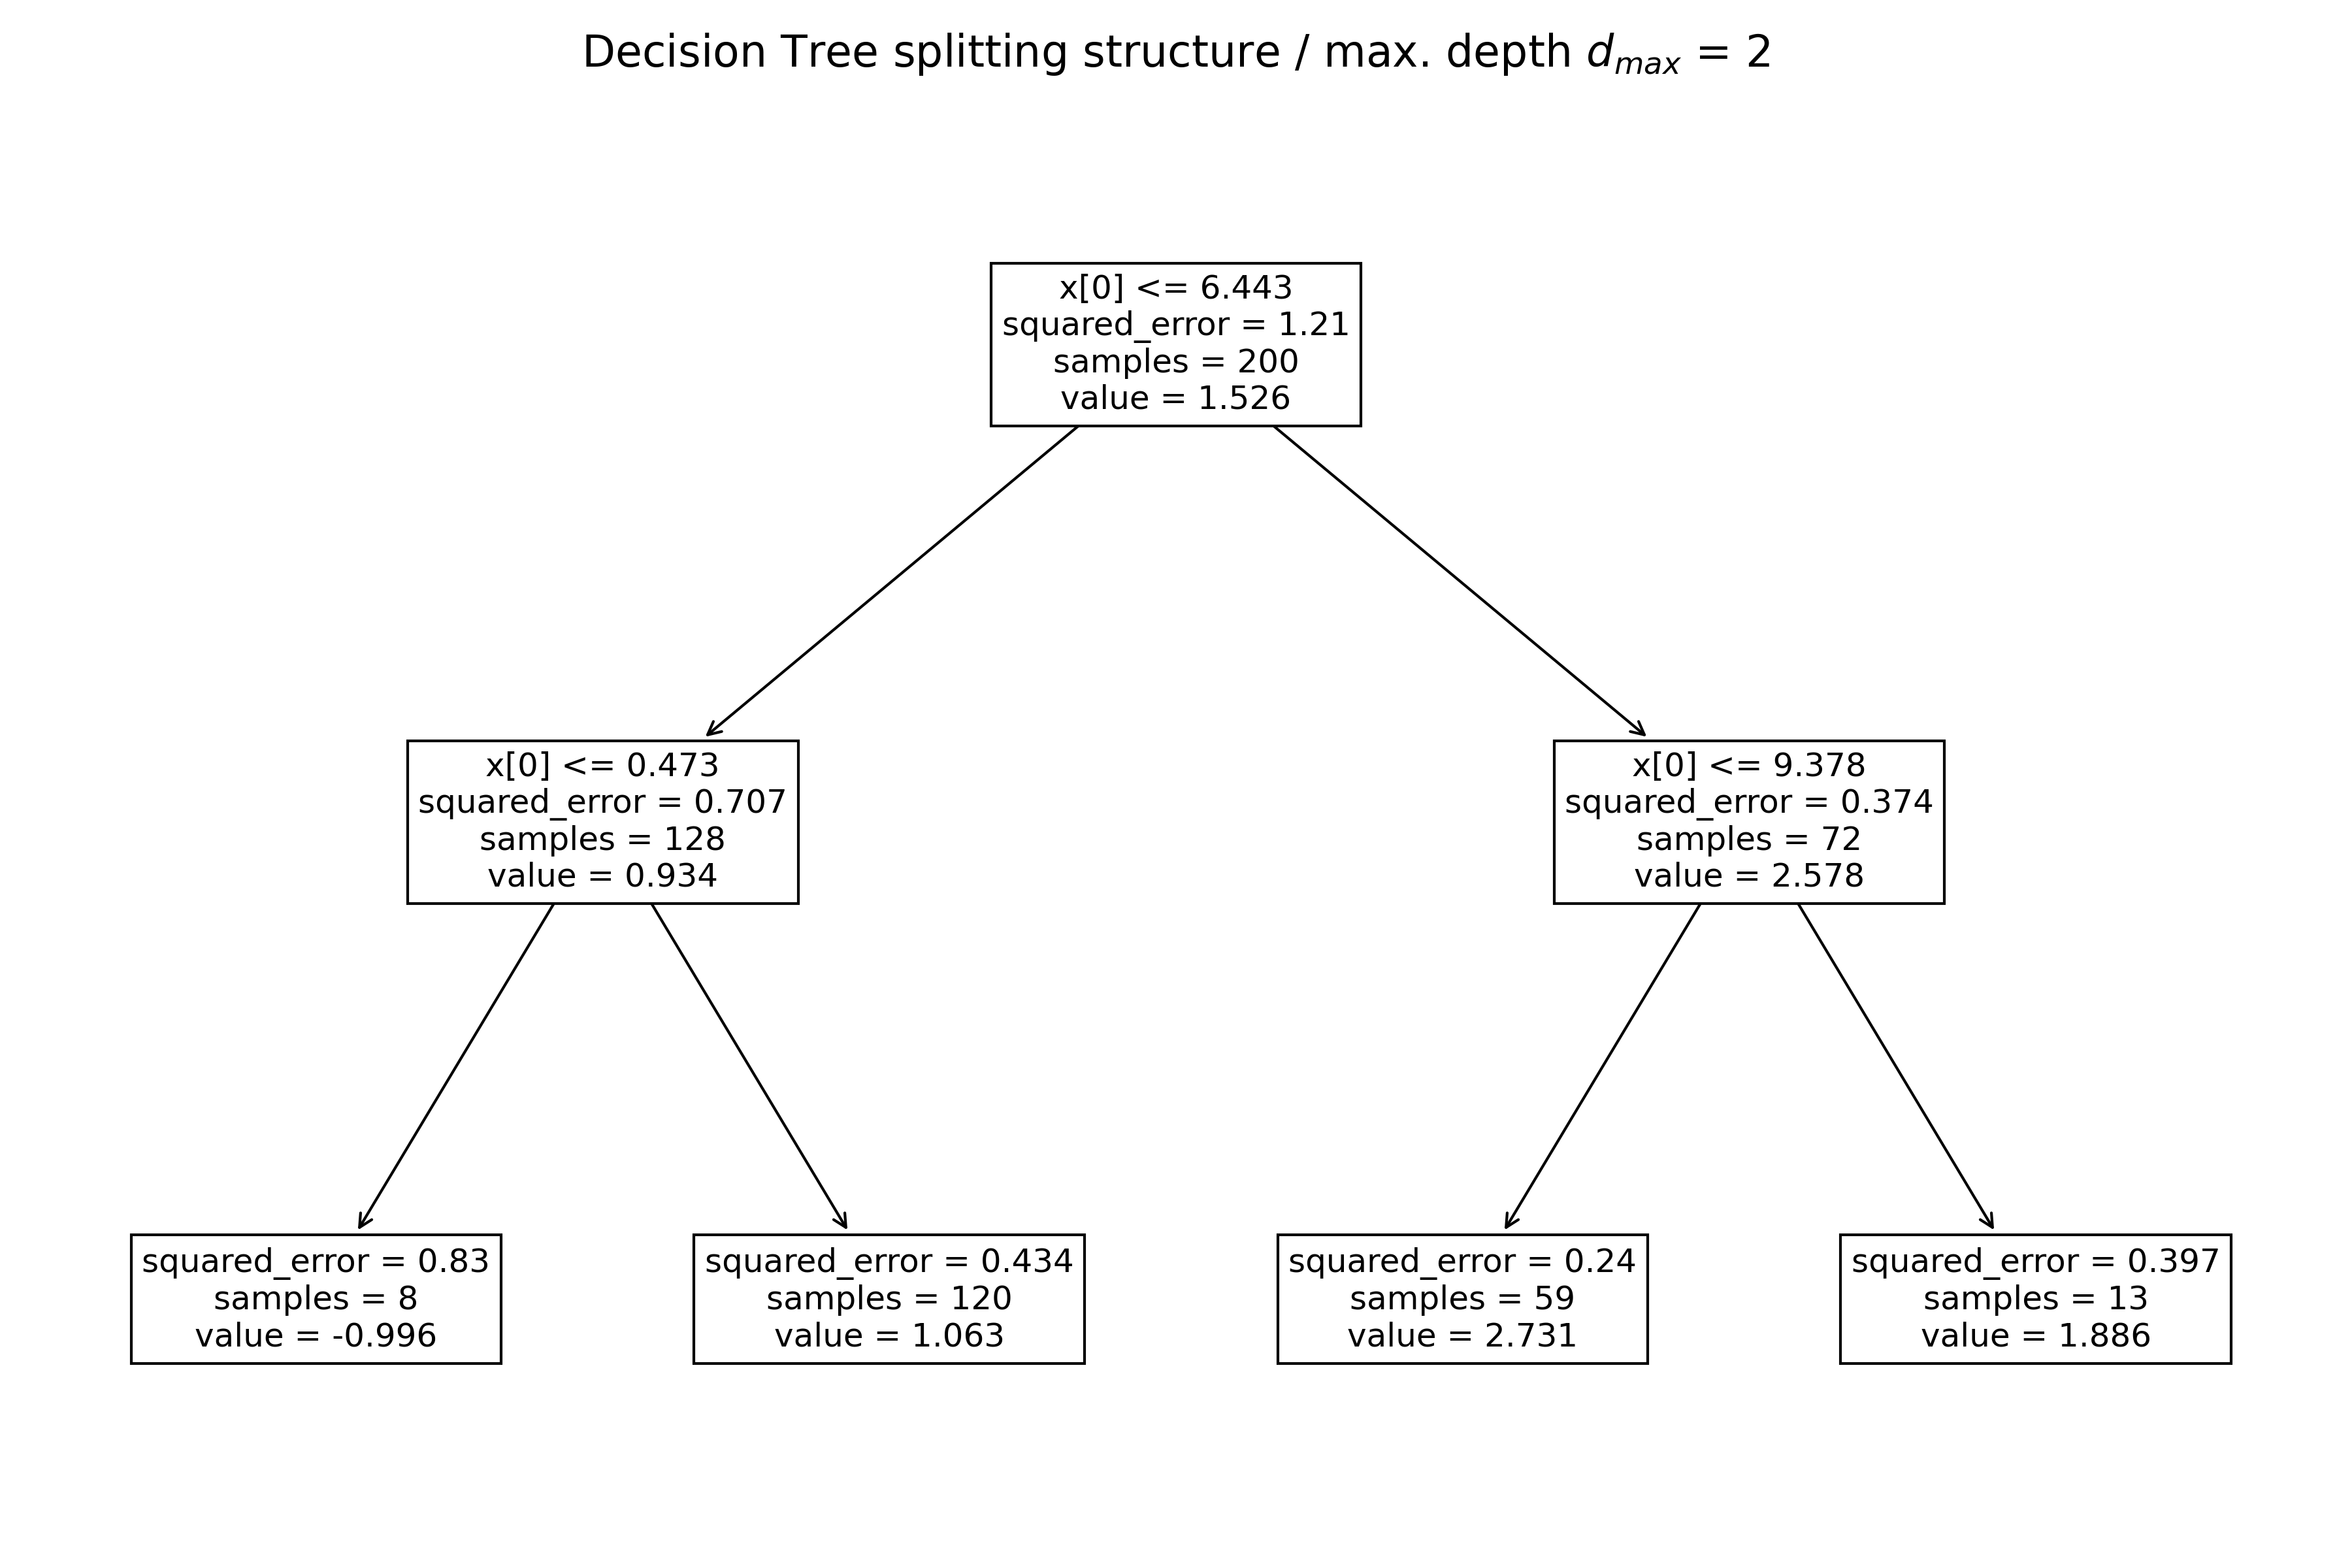
\includegraphics[width=1\textwidth,trim={0 0 0 0},clip]{figures/decision_tree_splitting_structure_md=2.png}
\caption[Decision Path / Two Layers]{Decision Path / $d_{max} = 2$}
\label{fig: dt_split_2} 
\end{minipage}
\end{figure}
\\
In addition the SKLEARN module \cite{Scikit2023} is also shown in the plots which results in the same splitting rules.
%%%%%%%%%%%%%%%%%%%%%%%%%%%%%%%%%%%
\newpage
\subsection{Hyperparameter optimization}
The right hyper-parameters are key for finding the optimal function approximation that minimizes the given cost function the best in terms of a ``scoring metric``. As stated in section [\ref{sec: cross_validation}] the uninformative gridsearch strategy evaluates all combinations of parameter constellations (grid points). By using two hyper-parameters for the GBM-DT model this would result in a two dimensional grid (surface). In the following figure [\ref{fig: gbm_hyper_matrix}] some combinations for the scalar test-function $F(x)$ prediction problem are shown.
\begin{figure}[!htpb]
    \centering
    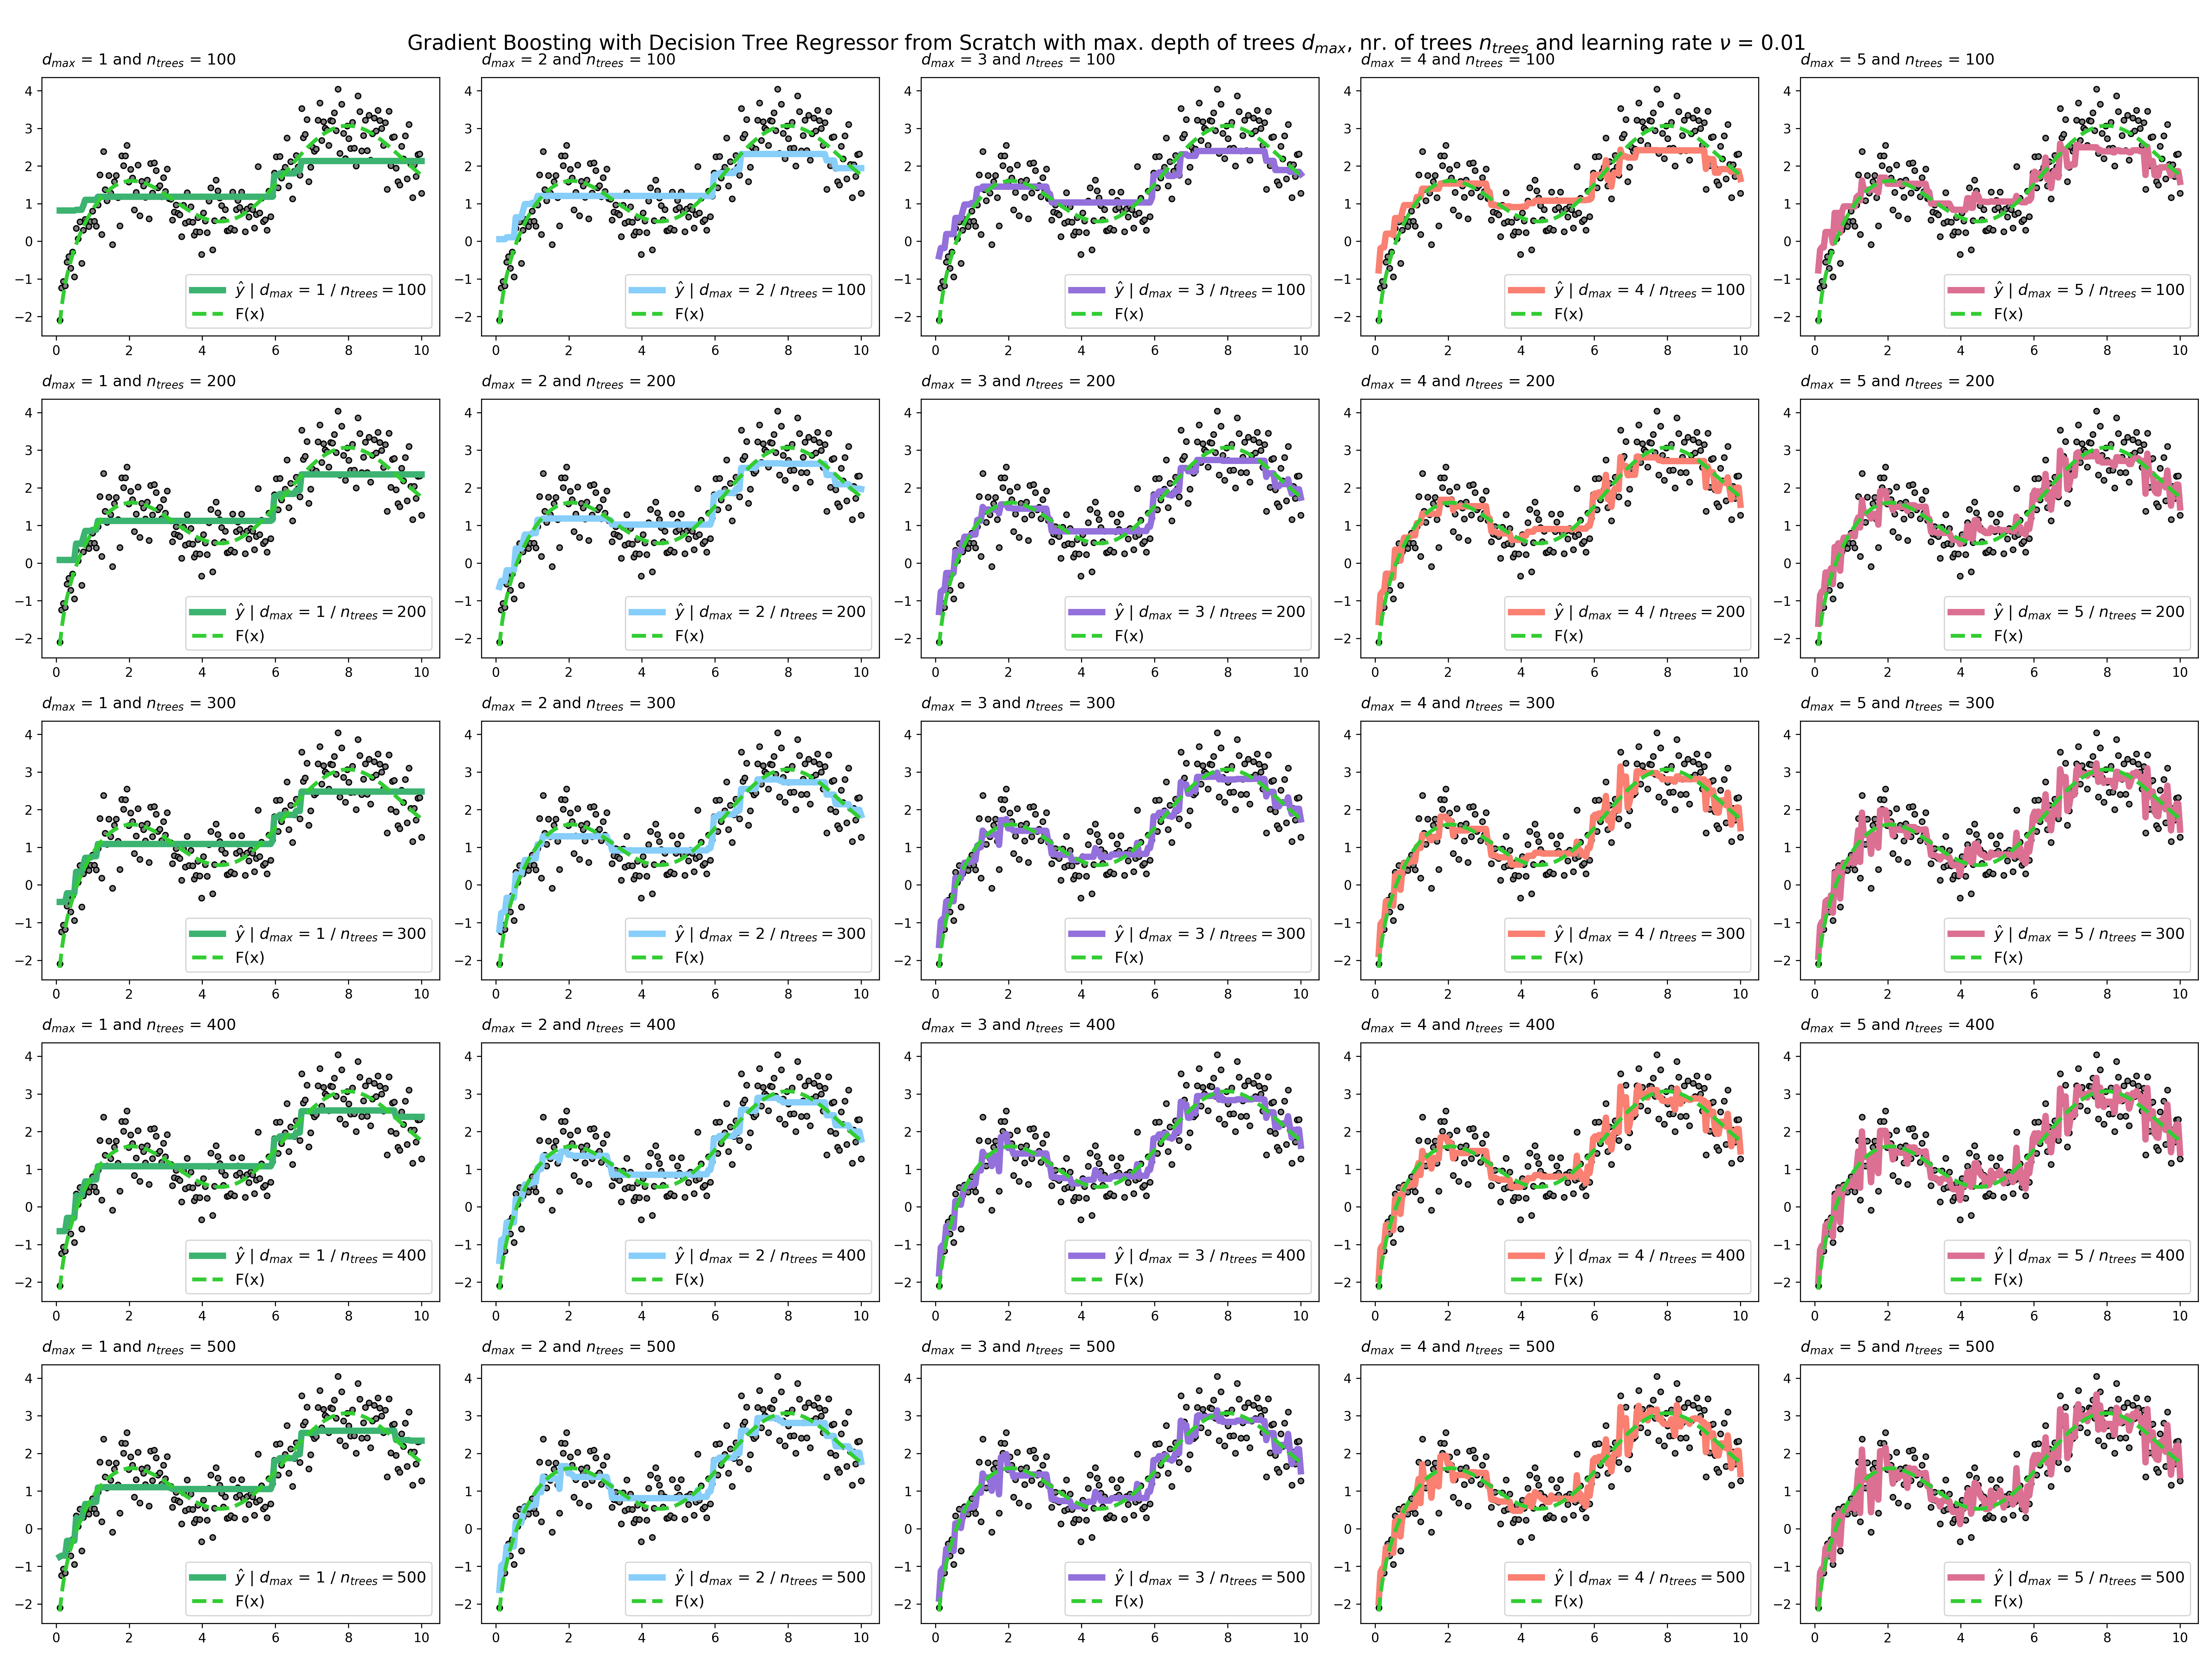
\includegraphics[width=1\textwidth,trim={0.5 0 0 0},clip]{figures/gbm_with_decision_tree_various_parameters.png}
    \caption[GBM-DT hyperparameter matrix]{GBM-DT hyperparameter matrix for maximal depth $d_{max}$ and number of trees $n_{trees}$ / inital sample points and fitted GBM-DT model}
    \label{fig: gbm_hyper_matrix}    
\end{figure}
We can see that the tree depth increases the approximation complexity and results more likely in overfitting. This is because the model learns relations very specific to the particular sample and will prioritize the given depth information (noise) too high. Increasing the number of trees or boosting rounds $n_{trees} = m$ expand the additive modeling structure and takes more samples points into account. Because of the high dimensional hyper-parameter space the informed cross validation method (BO) for finding the optimal parameter configuration is used.
As described in section [\ref{sec: bayesian_opt}] the idea is to learn from a given parameter combination which has been tested on the model over the training set and predicting the next better combination.
%%%%%%%%%%%%%%%%%%%%%%%%%%%%%%%%%%%%%%%%%%%%%%%%%%%%%%%%%%%
\subsection{Bayesian Optimization Schematic over an Test Objective Function}
But firstly the Bayesian Optimization Framework will be analyzed from scratch. For testing the framework we'll treat a known analytical expression of the test objective function $F(x)$ as ``black-box`` function.
\begin{center}
    $F(x) = - \text{sin}(3x) - x^2 + 0,7 \cdot x + \Theta \cdot \mathcal{N}(\cdot)$ 
\end{center}
\begin{figure}[htbp]
\begin{minipage}[t]{7cm}
\vspace{0pt}
\centering
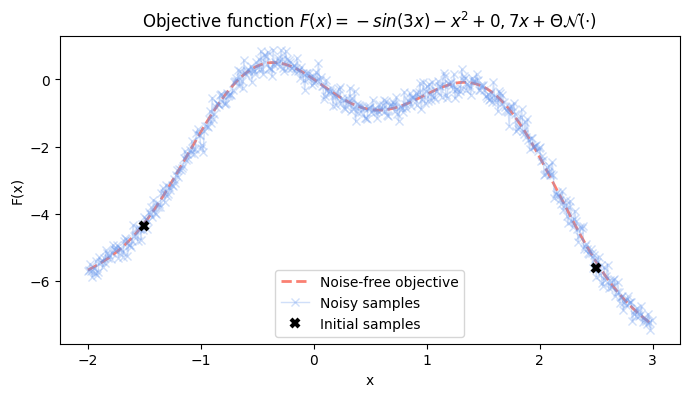
\includegraphics[width=1\textwidth,trim={0 0 0 0},clip]{figures/bayesian_optimization_from_scratch_objective.png}
\caption[Test Objective Function for Bayesian Optimization]{Test Objective Function $F(x)$ for Bayesian Optimization}
\label{fig: bo_objective}    
\end{minipage}
\hfill
\begin{minipage}[t]{5cm}
\vspace{0pt}
\centering
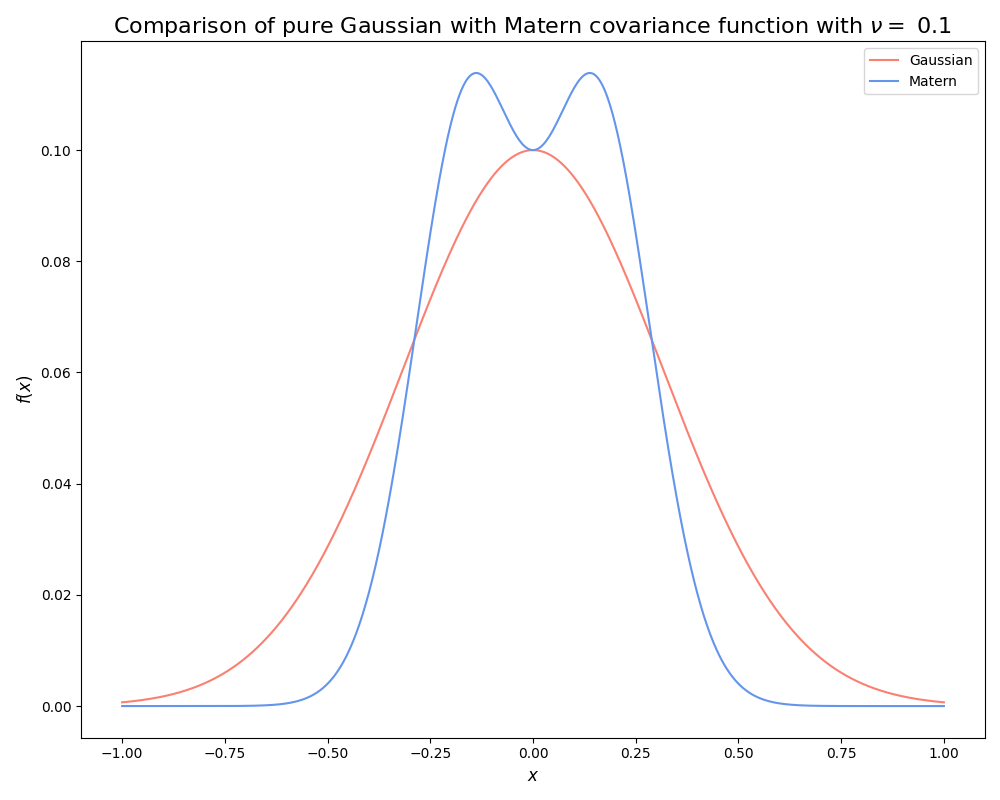
\includegraphics[width=1\textwidth,trim={0 0 0 0},clip]{figures/covariance_function_matern_gaussian.png}
\caption[Covariance functions for BO kernel]{Gaussian and Matern covariance function for BO kernel with $\nu = 0,1$}
\label{fig: covariance_functions} 
\end{minipage}
\end{figure}
Furthermore a Gaussian noise $\mathcal{N}(\cdot)$ we'll be added to simulate a real-world ``objective -function`` [Fig. \ref{fig: bo_objective}]. 
Through iteration we'll try to approximate this ``black-box`` function through a Bayesian Optimization framework with Gaussian Processes as surrogate model. Because of simplicity we'll deal with a one-dimensional input domain $x \in \mathcal{X}$.
As Frazier et al. [Ref. \cite{Frazier2018}] described GP take a significant role in optimization problems, therefore a specific covariance function is often used when dealing with noisy data, namely the ``Matern Kernel`` [Fig. \ref{fig: covariance_functions}]. The reason is because one can control the smoothness over flexibility of the GP model. In addition the Matern Kernel also provides more robustness because it handles noisy data observations better. \\
The goal is to find the global optimum of this objective function in a small number of steps. We'll set the bounds of the domain to $\mathcal{X} = [-2, 3]$ and the initial sample points to $\mathcal{X}_{inital} = \{-1,5;+2,5\}$. The noise parameter will be set to $\Theta = 0,2$.
The Bayesian optimizer we'll be implemented as described in section [\ref{sec: bayesian_opt}] with Expected Improvement as acquisition function and for optimization the Quasi-Newton method with defined bounds we'll be used [Code Ref. \href{https://github.com/probabilis/bs_ml/tree/master/from_scratch}{Github repository}]. \\
The left plot [Fig. \ref{fig: bo_iterations}] shows the noise-free objective function, the surrogate function which is the GP posterior predictive mean, the 95\% confidence interval of the mean and the noisy samples obtained from the objective function so far. The right plot [Fig. \ref{fig: bo_iterations}] shows the corresponding acquisition function at each iteration step and the vertical line in both plots shows the proposed sampling point for the next iteration which corresponds to the maximum of the acquisition function. In figure [\ref{fig: bo_convergence_plot}] two convergence plots over the iterations are given.
On the first plot the distance $\Delta{x}$ between consecutive sample points $x_i$ is shown. On the second plot the resulting objective function values $\tilde{F}(x)$ over the iterations is shown, which flattens because consecutive sample points $x_i$ get narrower in the domain $\mathcal{X}$. It is immediately visible that the distance shrinks down with ongoing iterations, which is a good sign for finding the maximum. Nevertheless this convergence could theoretically be a local maximum and not the global.
\begin{figure}[!htpb]
    \centering
    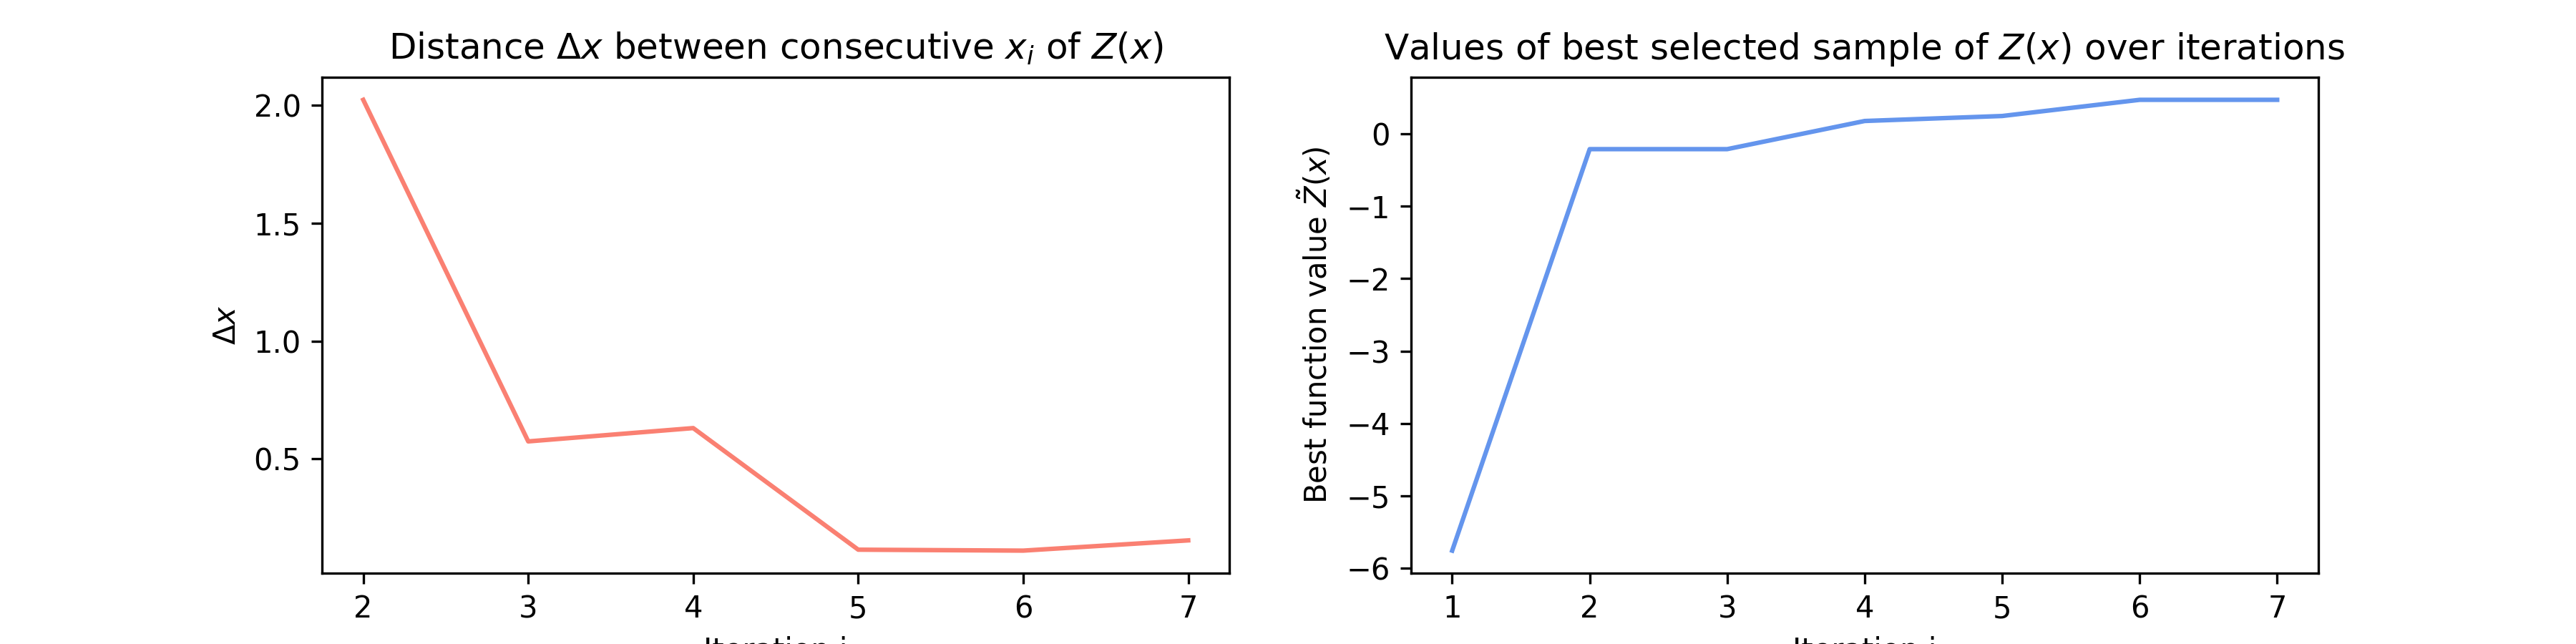
\includegraphics[width=1\textwidth,trim={0 0 0 0},clip]{figures/bayesian_optimization_from_scratch_convergence_plot.png}
    \caption[Bayesian Optimization convergence plot]{Bayesian Optimization convergence plot of test-objective function}
    \label{fig: bo_convergence_plot}    
\end{figure}
\\
Interesting is here the balanced trade-off between exploration and exploitation. Initially the optimizer based on the two sample points drives the search direction to the left side but exploration allows the algorithm to escape from the local optimum and find the global optimum on the middle-left side. Additionally the sampling point proposals often fall within regions of high uncertainty (exploration / iteration 3) and are not only driven by the highest surrogate function values (exploitation / like it is visible on iteration 4). After 7 iterations the global maximum of the objective function is found.
\begin{figure}[!htpb]
    \centering
    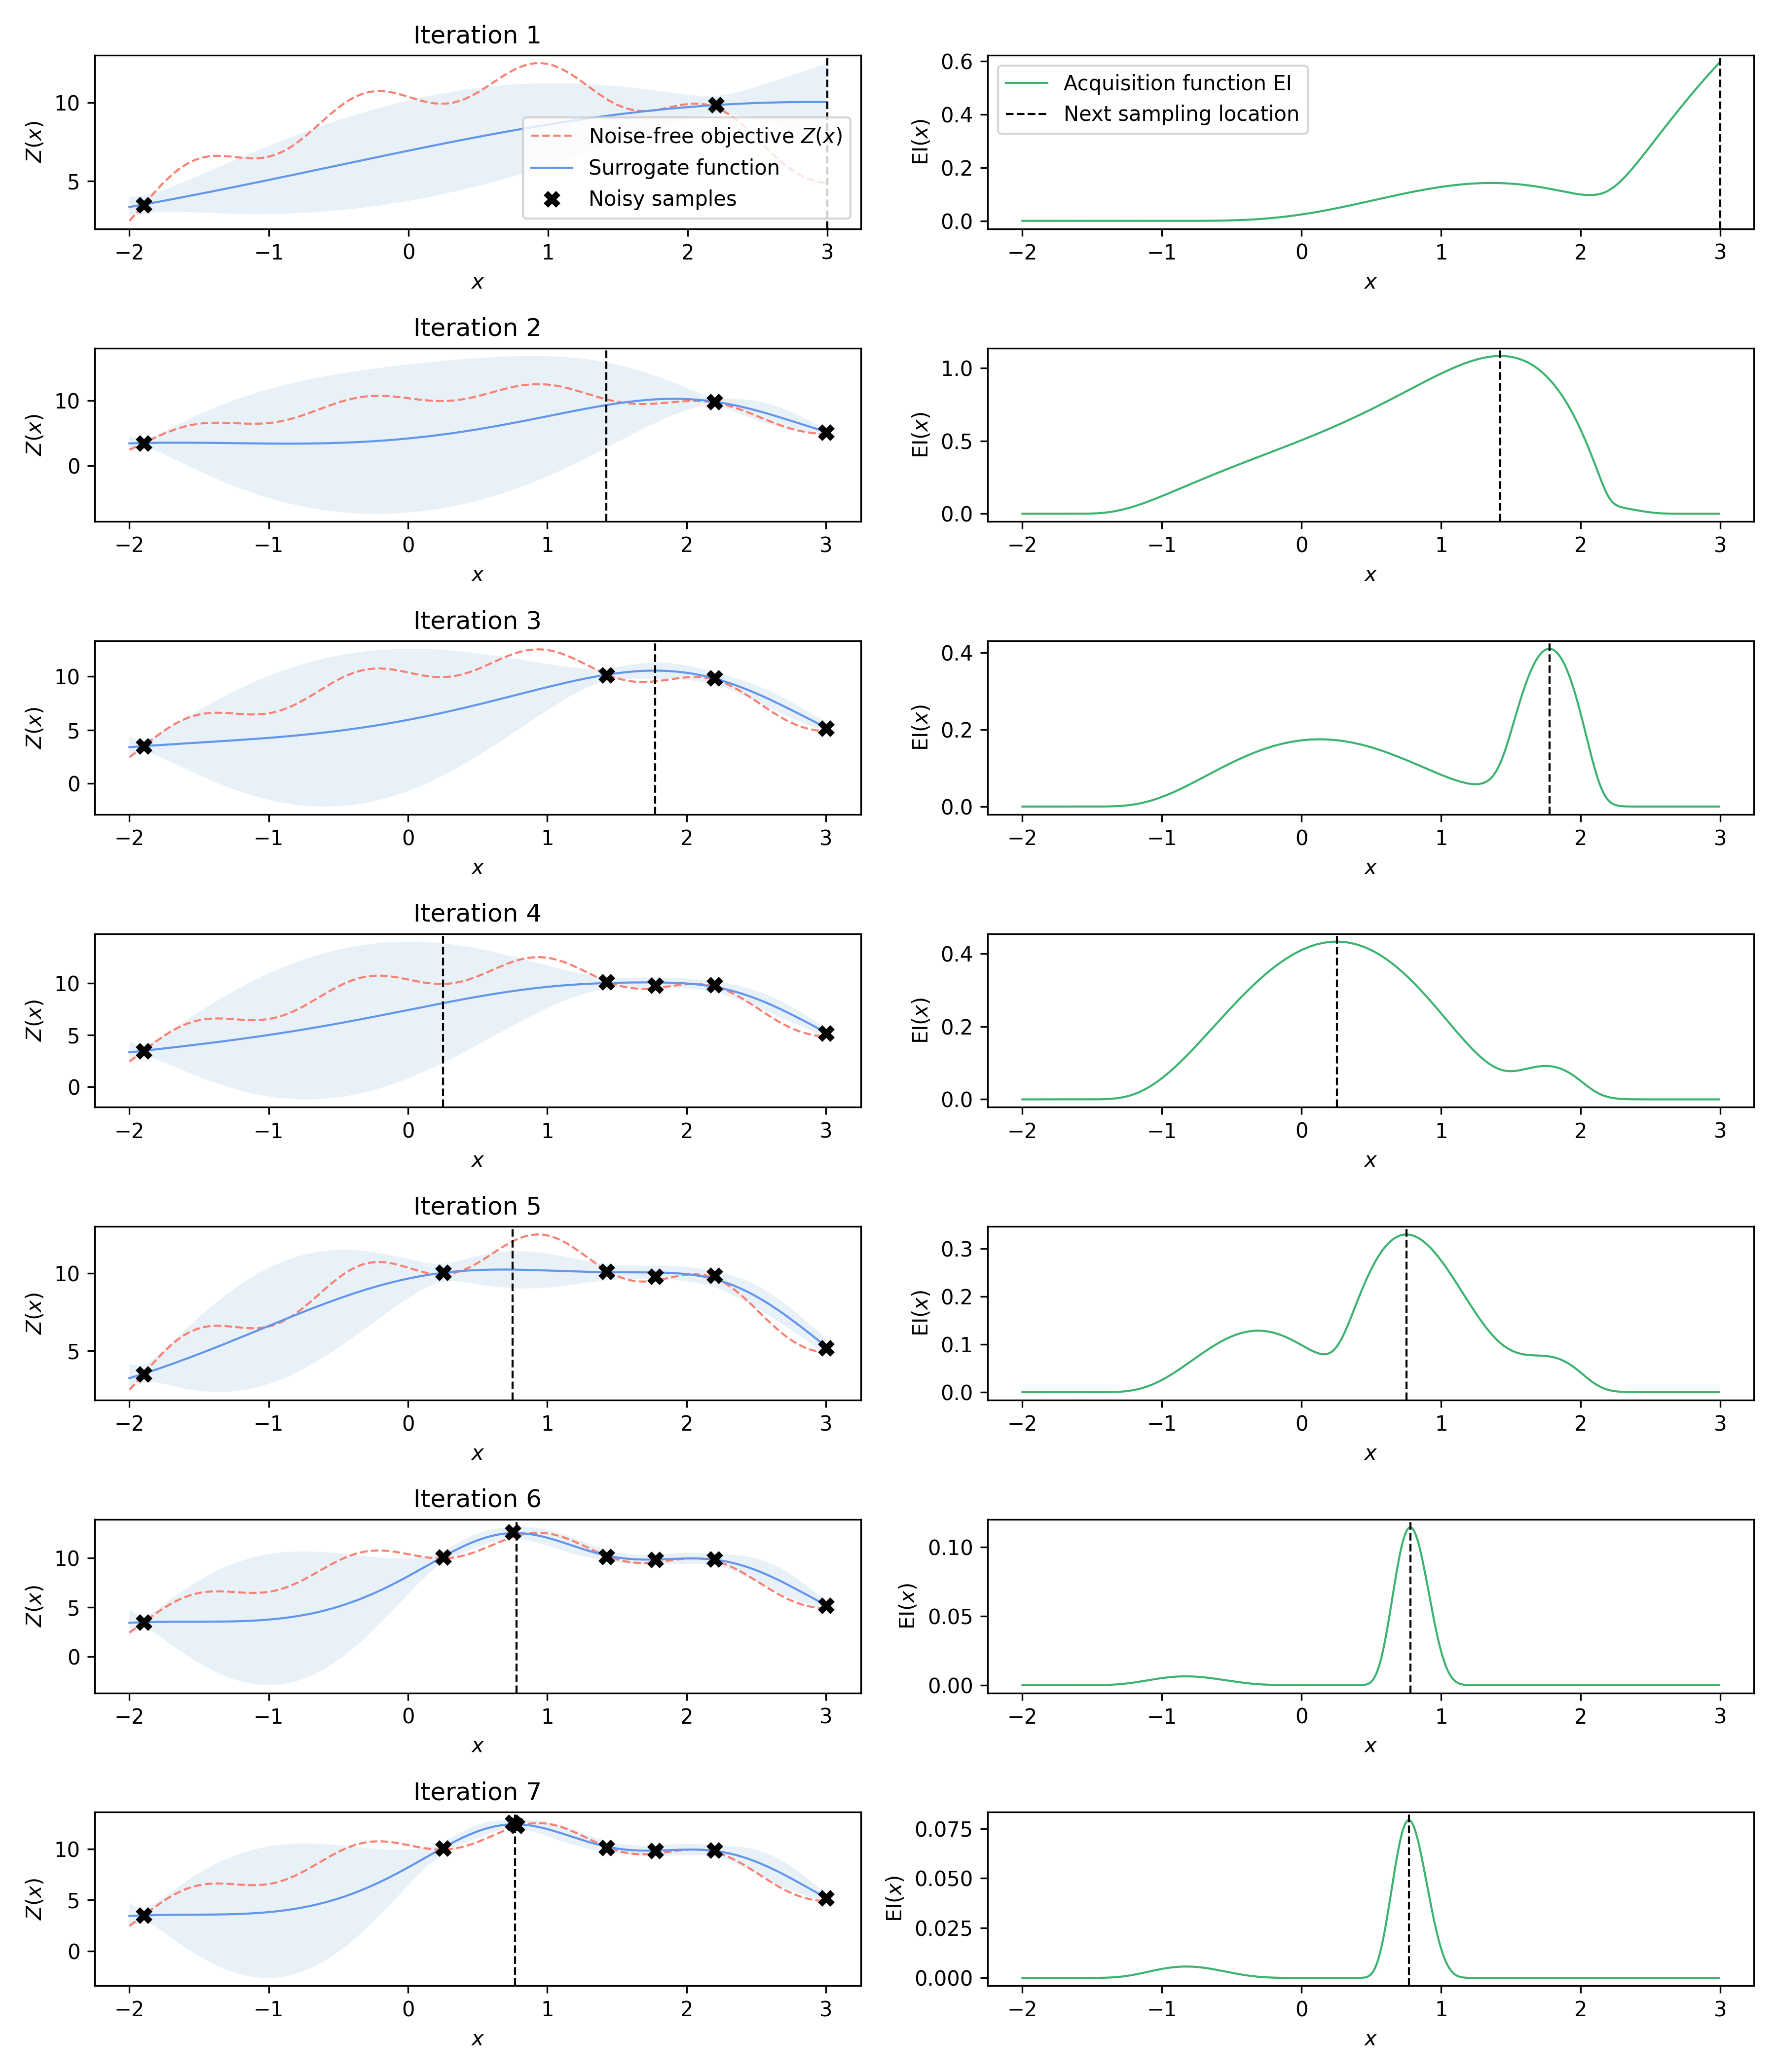
\includegraphics[width=1\textwidth,trim={0 0 0 0},clip]{figures/bayesian_optimization_from_scratch_iterations.png}
    \caption[Bayesian Optimization Iterations]{Bayesian Optimization iterations with Gaussian Prior for predicting the Objective Function $F(x)$}
    \label{fig: bo_iterations}    
\end{figure}
%%%%%%%%%%%%%%%%%%%%%%%%%%%%%%%%%%%%%%%%%%%%%%%%%%%%%%%%%%%%%%%%%%%%%
\newpage
\subsection{Optimal Hyperparameter configuration for test function problem}
\label{sec: bayesian_opt_test}
Given the scalar testfunction from beforehand 
\begin{center}
    $F(x) = \text{sin}(x) + \text{ln}(x) + \Theta \cdot \mathcal{N}(\cdot)$
\end{center}
we'll try to optimize the objective test function over the hyperparameter space to get the best possible pair of parameters to fit our function. Therefore we'll use the most inherent hyperparameters of Gradient Boosting Methods where the base learners are based on Decision Trees, as the algorithm proposed in [Alg. \ref{alg: gb_ls_algo}]. 
\begin{itemize}
    \item Learning Rate $\nu$
    \item Maximal depth of trees $d_{max}$
    \item Number of Trees / Iterations $n_{trees} = m_{estimators}$
    \item Colsample by Tree $\nu$
\end{itemize}
Whereby we've introduced the learning rate $\nu$ as a parameter for shrinkage for regularization [\ref{eq: gb_algo_shrinkage}]. The maximal depth of trees $d_{max}$ resulted in the tree-structured design of our bases learners [\ref{alg: tree_growing_algo}]. Through the additive modeling schematic from our GB machine we'll use consequently the number of trees $n_{trees}$. Colsample by tree $\epsilon$ comes from \textit{Random Forests}. Because of the additive modeling behavour the model acts as ensemble of many trees. Therefor we could ``randomly`` assign training samples to each tree (bootstrapping)  and building each tree's node only considering a random subset of the attributes. So for earch tree in a random forest one selects a random sample from the dataset to train the tree and for each node of this tree use a random subset of the features (if there are more than one). The advantage is here to reduce overfitting and decorrelate the trees best possible.  \\
First the boundaries have to be set on each specific parameter to provide the optimizer the function space where the maximum should be found.
\begin{itemize}
    \item Learning Rate $\nu \in  [0,01 ; 0,2]$
    \item Maximal depth of trees $d_{max} \in [1; 10]$
    \item Number of Trees $n_{trees} \in [100; 20000]$
    \item Colsample by Tree $\epsilon \in [0,1; 1]$
\end{itemize}
Through the Bayesian Optimizer we'll predict where the global-maximum of our objective function $F(\nu,d_{max},n_{trees},\epsilon)$ lies and therefor what the best configuration-set of hyperparameters are over the training set. Because of simplicity we'll use therefore the open-source built Python library \href{https://github.com/bayesian-optimization/BayesianOptimization}{Bayesian Optimization}, which Nogueira et al. \cite{Nogueira2014} built. \\
The proposed acquisition functions in section [\ref{sec: bayesian_opt}] are all built-in and there's the possibility to iterate through the Bayesian prediction process. Two main parameters have to be chosen:
\begin{itemize}
    \item $n_{iter}$ : Number of steps of the Bayesian Optimization process
    \item $init_{points}$ : Number of steps of random exploration one wants to perform (random exploration helps to diversify the exploration space)
\end{itemize}
Through sub-sampling the dataset via 5-fold cross validation (CV) strategy (scikit-learn library) we can generalize the function to an independent dataset as discussed in section [\ref{sec: cross_validation}]. We can use this CV-metric to evaluate the scoring of our parameter set which we've optimized through predicting the objective function. We'll use the standard scorer function, the quadratic loss function $L_2$ for evaluation the score metric.
\begin{figure}[!htpb]
    \centering
    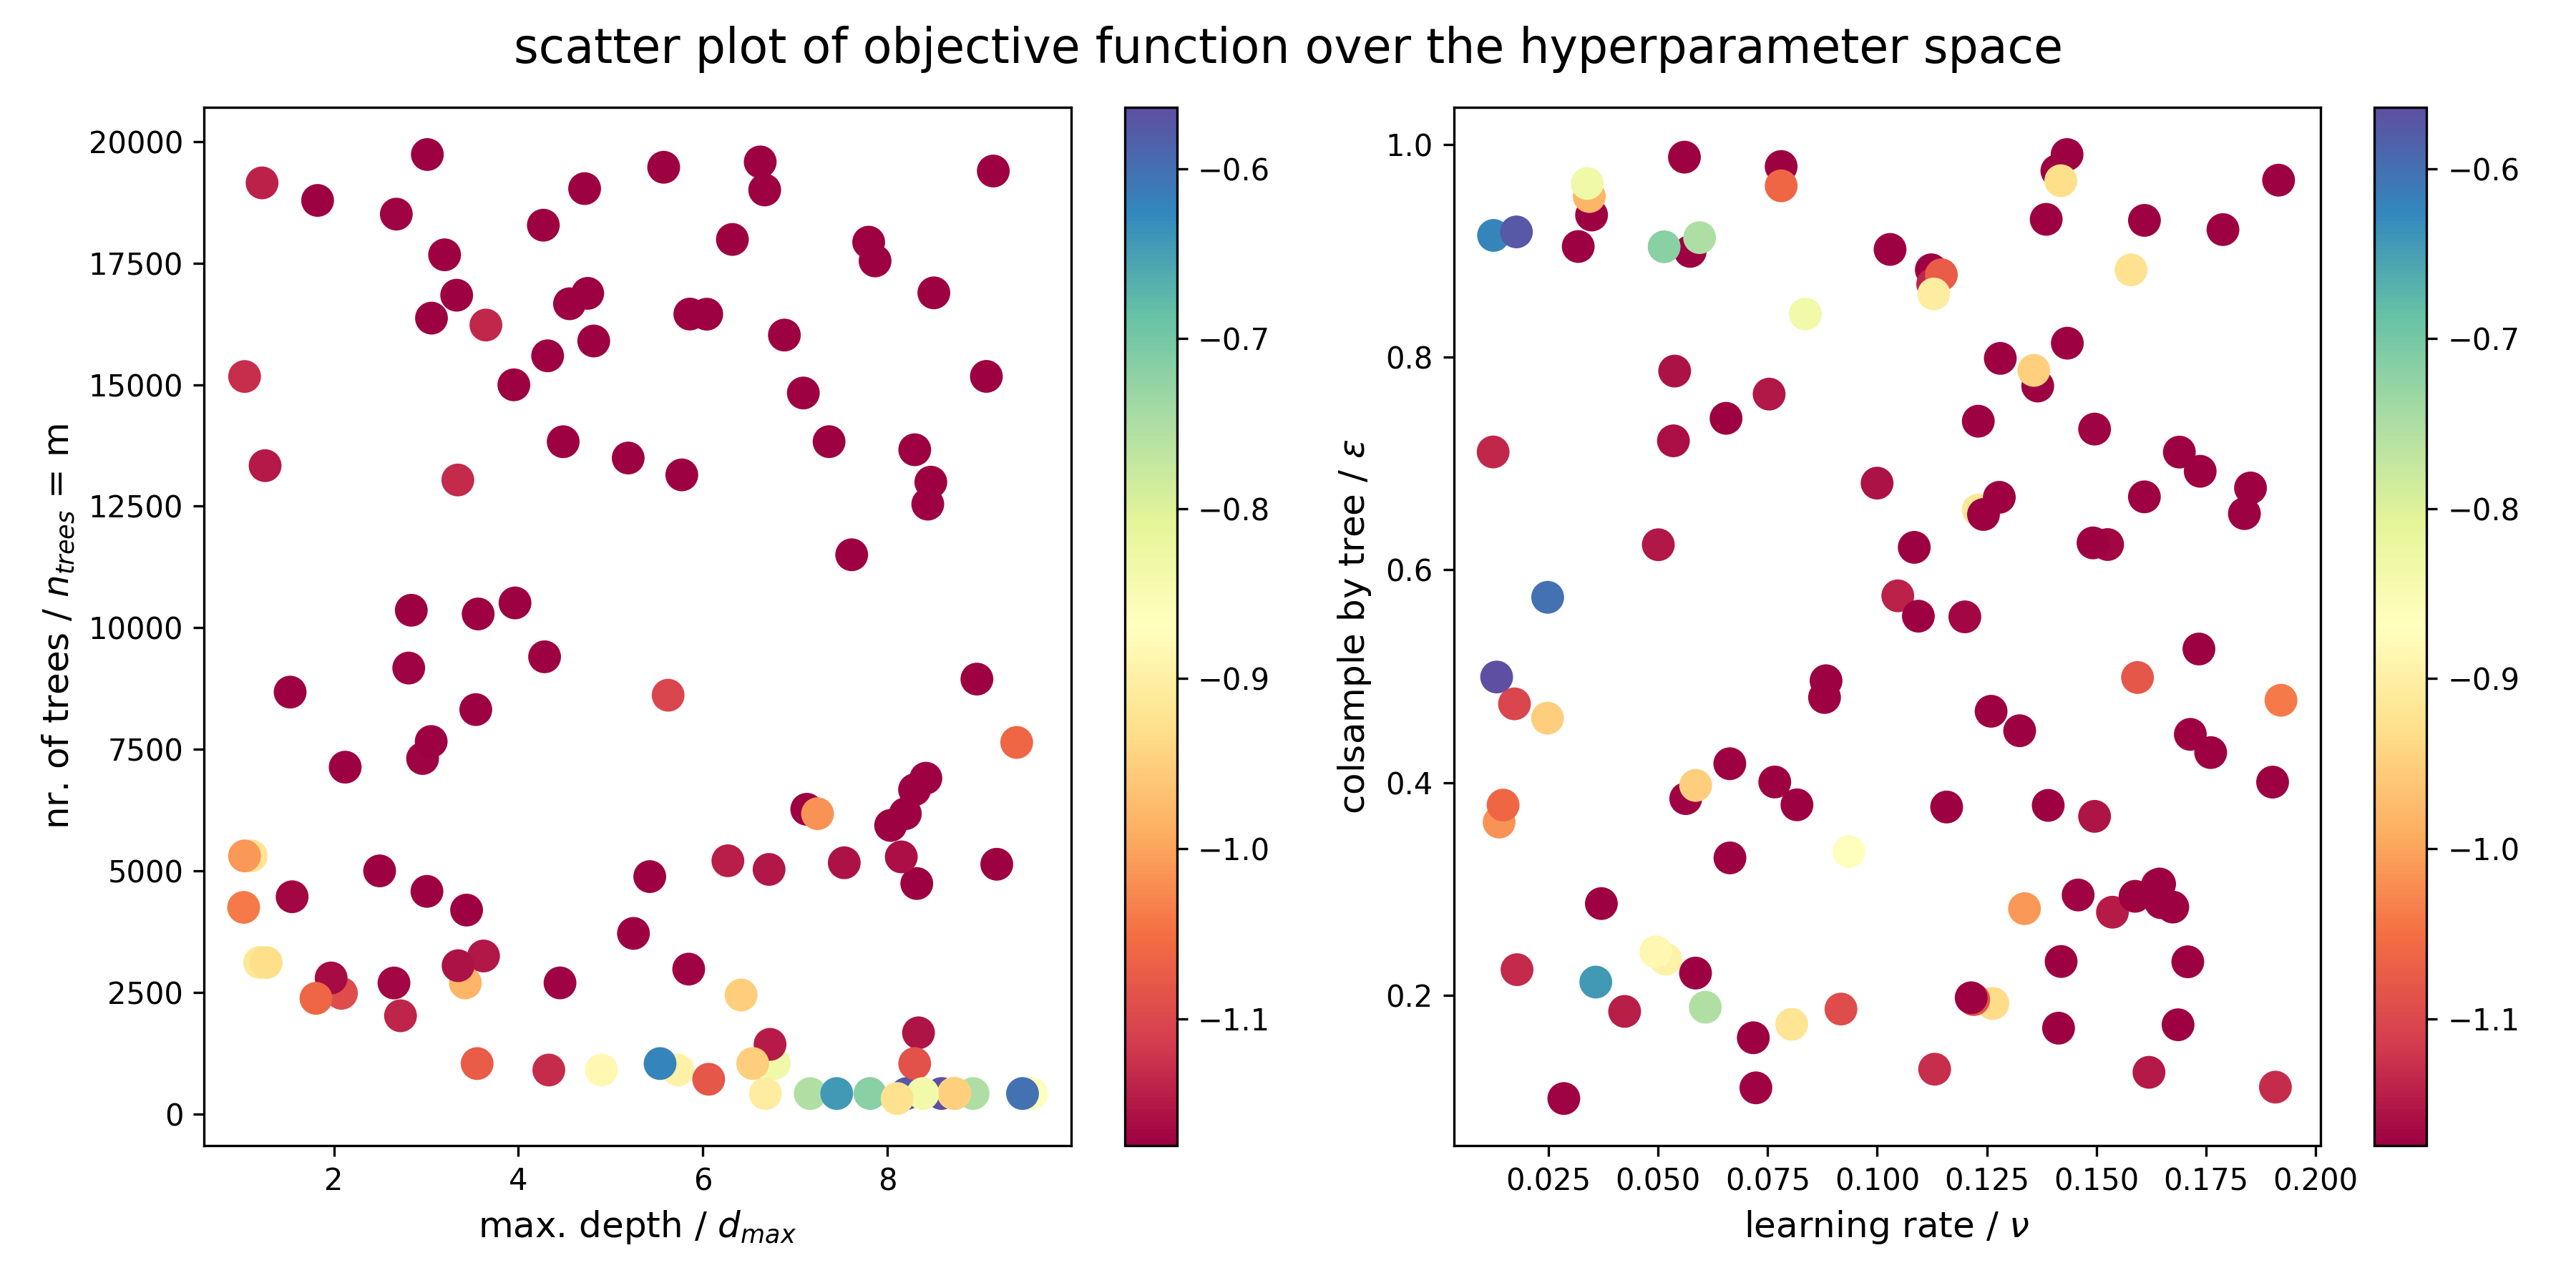
\includegraphics[width=1\textwidth,trim={0 0 0 0},clip]{figures/gbm_with_decision_tree_hyperparameters_scatter_plot.png}
    \caption[Bayesian Optimizations iterations]{BO of the objective function over their hyperparameters from the initial scalar-test function with $n_{iter}$ = 10 and $init_{points}$ = 100}
    \label{fig: gbm_dt_scatter_plot}    
\end{figure}
\\
We can extract that there's definitely a section in each hyperparameter domain where the objective function gets maximized. Nevertheless we can obtain that there are also local optima which may not result in the best possible solution. When dealing with hyperparameter optimization one can prevent this by:
\begin{itemize}
    \item use a wider search space over the hyper-parameter domains
    \item offer a wide field of random initialization samples
    \item prioritize high-impact hyperparameters like learning rate, maximal tree depth or the number of trees
    \item using an ensemble strategy for combining results over multiple optimization tasks
\end{itemize}
Therefore we may not get only one parameter-configuration which may fit our needs but either more. We can use multiple test runs to confirm our initial combination of parameters. The resulting dupel of hyperparameters which maximizes our objective function best possible are: \\
\begin{center}
    Learning Rate $\nu = 0,03$ / Maximal depth of trees $d_{max} = 1$ / Number of Trees $n_{trees} = 902$ / Colsample by Tree $\epsilon = 0,1$
\end{center}
The GBDT-model gets trained with the hyperparameters and results in following model $\tilde{y}(x)$ over the domain $\mathcal{X}$ [Fig. \ref{fig: gbm_dt_best_par}].
\begin{figure}[!htpb]
    \centering
    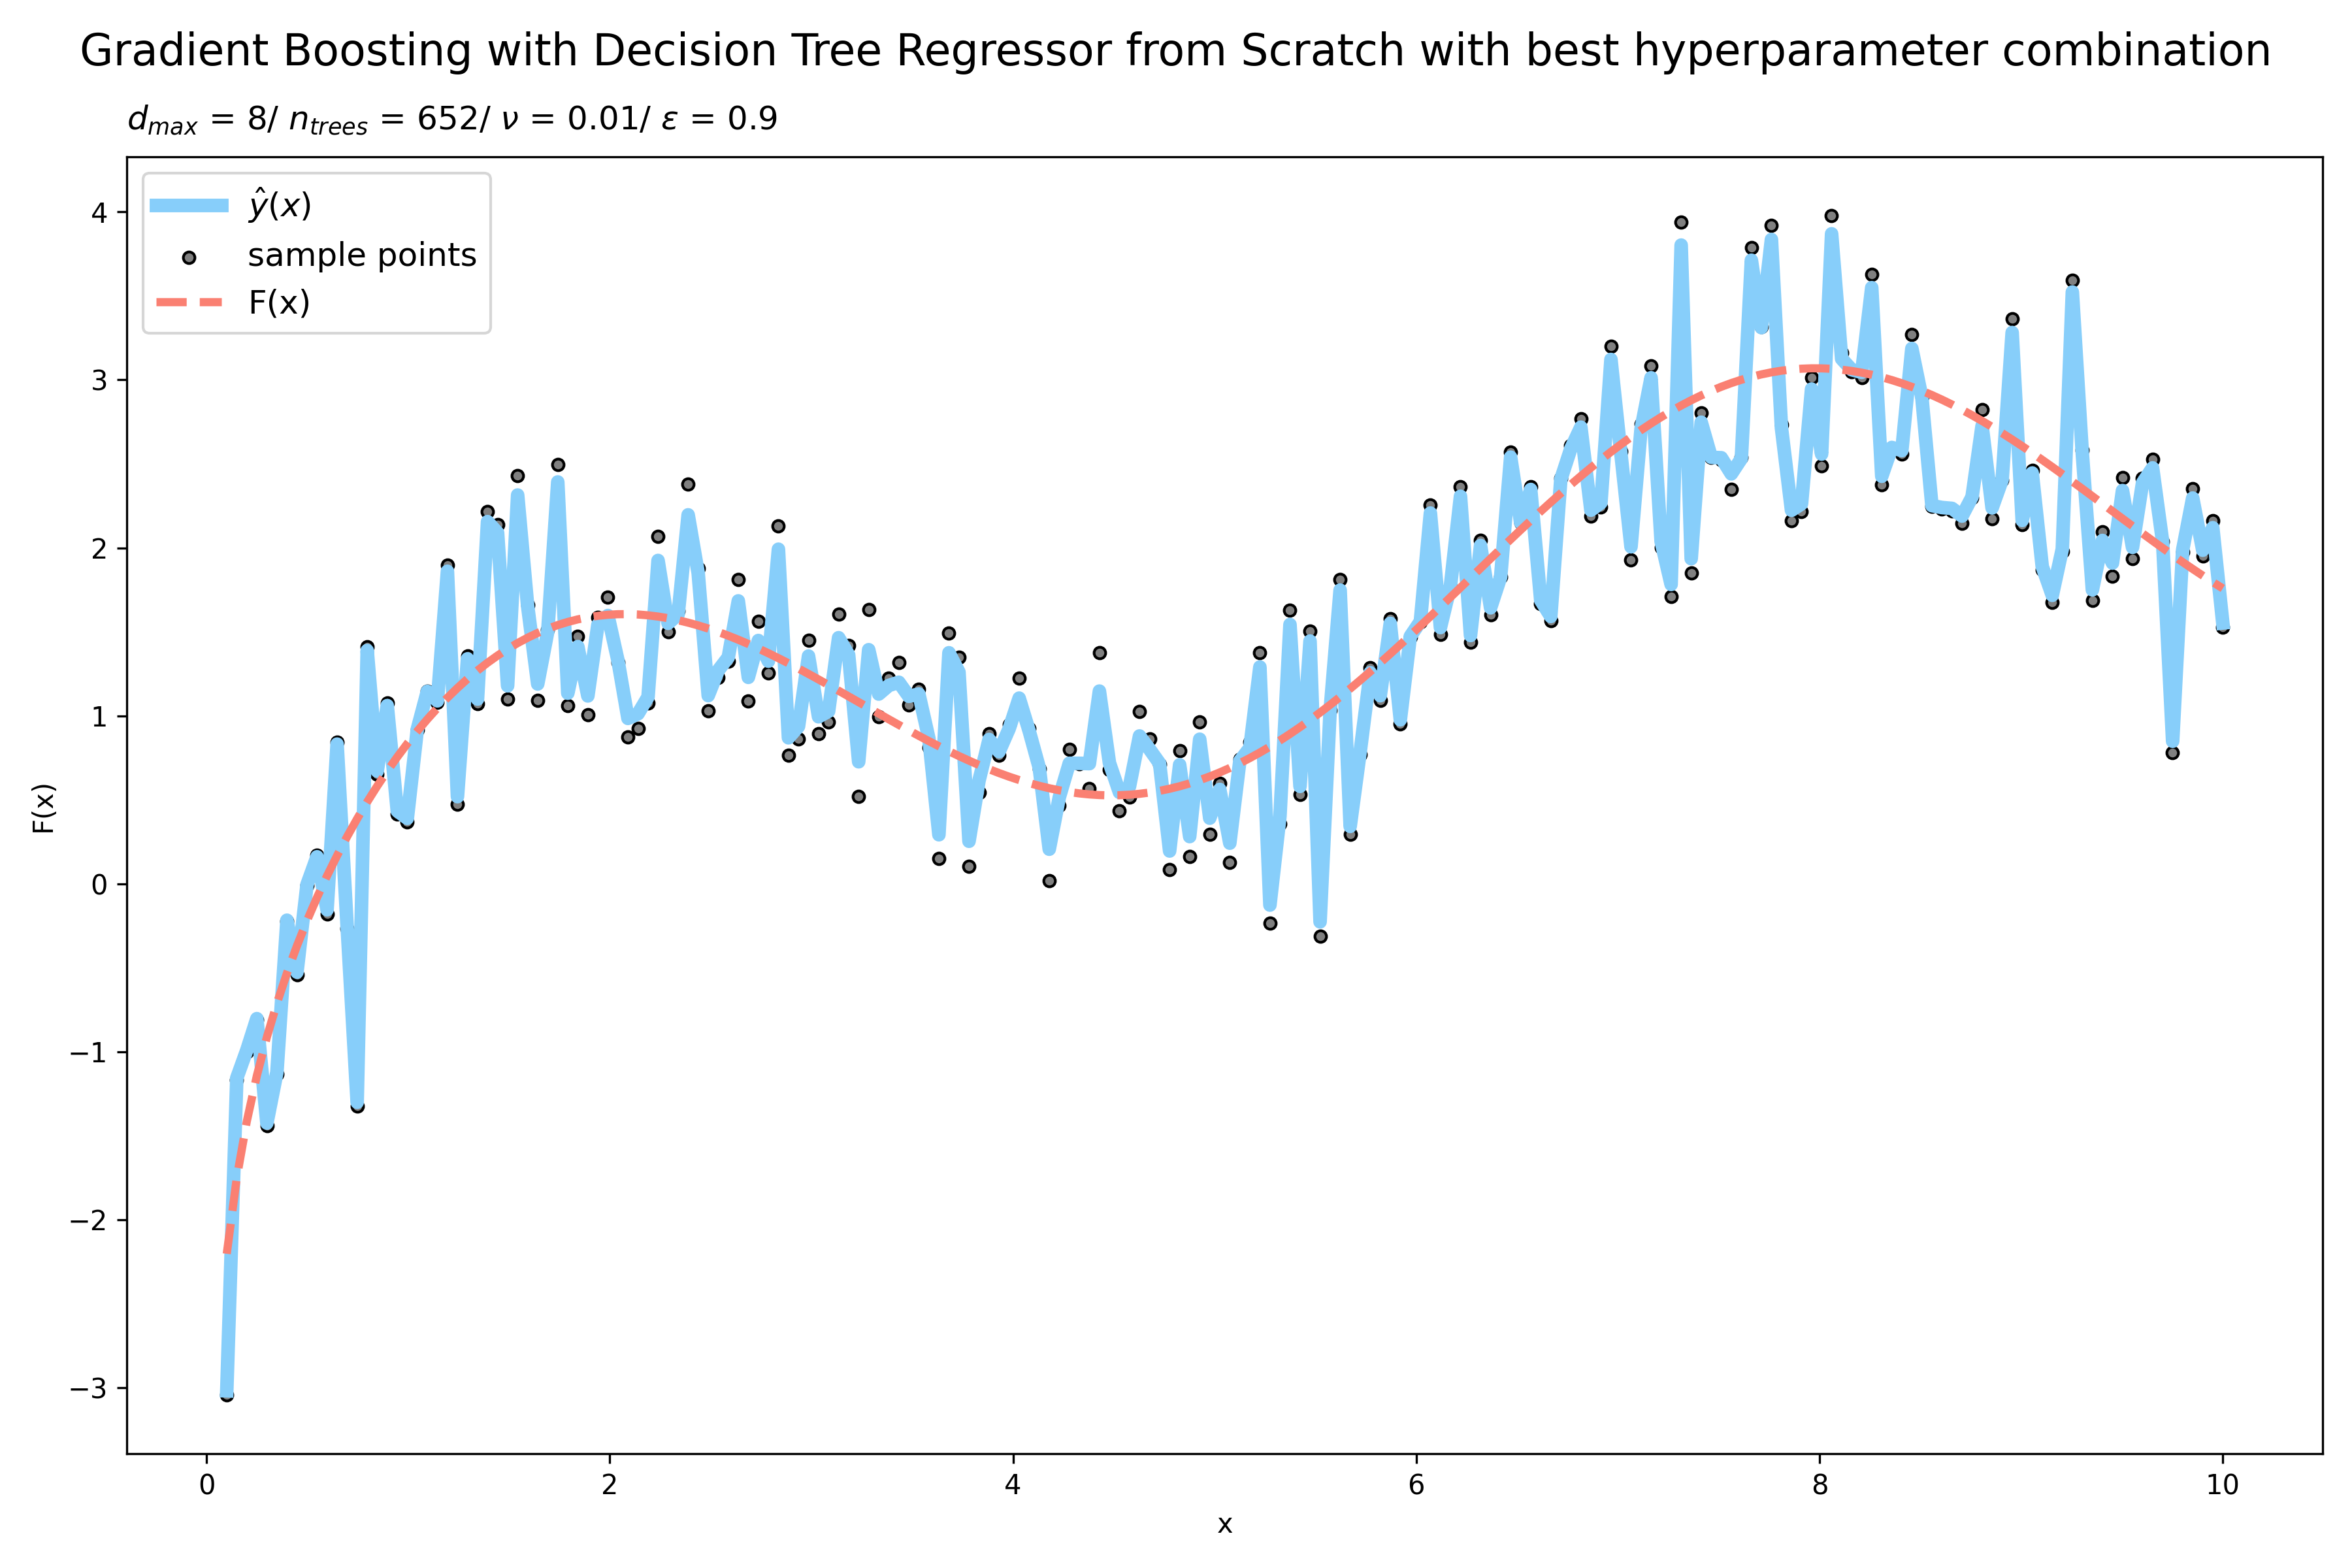
\includegraphics[width=1\textwidth,trim={0 0 0 0},clip]{figures/gbm_with_decision_tree_best_parameters.png}
    \caption[Best parameter configuration at GBM with Decision Trees on testfunction]{Best parameter configuration at GBM with Decision Trees on testfunction $F(x)$ with sample points and predicted $\tilde{y}(x)$}
    \label{fig: gbm_dt_best_par}    
\end{figure}
%%%%%%%%%%%%%%%%%%%%%%%%%%%%%%%%%%%%%%%%%%%%%%%%%%%%%
\newpage
\section{Real-world data problem approximation}
The goal is to analyze a real-world data problem and to build the best possible model (prediction) with the given toolkit of a GBM based on Decision Trees tuned by Bayesian Optimization. Because of our GBM design the dataset has to be pure regressional in terms of the contained values. The chosen dataset is from \href{https://numer.ai}{numer.ai}, the first decentralized hedge-fund of it's kind, which provides an anonymized normalized time-series table for free.
\subsection{Numer.ai dataframe}
The training-dataset consists of different encrypted \textit{id's} which corresponds to a stock at a specific time era of over more than 500 \textit{eras} (each era is exactly one week apart) with over 1000 \textit{features} and 20 different \textit{targets}. This results in single feature vectors with more than 5 million entries  [Fig. \ref{fig: numerai_dataset}]. 
\begin{figure}[!htpb]
    \centering
    \includegraphics[width=0.7\textwidth,trim={0 0 0 0},clip]{figures/numerai_dataset.png}
    \caption[Numer.ai dataset structure]{Numer.ai dataset structure [From \href{https://numer.ai/}{numer.ai}]}
    \label{fig: numerai_dataset}    
\end{figure}
The features describe the various quantitative attributes of the stock at the time (fundamentals like P/E ratio, technical signals like RSI, market data like short interest, secondary data like analyst rating..).
Features values are binned into 5 equal bins: $\{0;1;2;3;4\}$ and are overall subdivided in 8 different groups [also seen in Fig. \ref{fig: per_era_correlation}].  \\
The target represents an abstract measure of performance a fixed number of weeks into the future (20-day stock market returns). Specifically, it is a measure of ``stock-specific`` returns that are not ``explained`` by broader trends in the market, country, sector, or well-known ``factors``. Target values are binned into 5 unequal bins: $\{0; 0,25; 0,5; 0,75; 1,0\}$. This heavy regularization of feature and target values is to avoid overfitting as the underlying values are extremely noisy. \\
This huge amount of data measures in raw CSV format around 10 Gigabyte of data in the compressed \textit{parquet}-format around 1,8 Gigabyte. 
Additionally there is a validation dataset prepared for checking the model's performance before submitting the model. By submitting a robust machine learning model based on the provided data one get \textit{True Contribution} stake to overall meta-model which calculates contribution. This \textit{Stake-Weighted Meta Model} produces trading signals, as Richard Craib (Founder) stated in [\href{https://docs.numer.ai/numerai-tournament/scoring/true-contribution-tc}{numer.ai}], whereby the convex optimization machine turns those signals into a portfolio by constructing risk factors [Fig. \ref{fig: numerai_true_contribution}]. 
\begin{figure}[!htpb]
    \centering
    \includegraphics[width=1\textwidth,trim={0 0 0 0},clip]{figures/true_contribution.png}
    \caption[Numer.ai True Contribution schematic]{Numer.ai True Contribution schematic [From \href{https://docs.numer.ai/numerai-tournament/scoring/true-contribution-tc}{numer.ai}]}
    \label{fig: numerai_true_contribution}    
\end{figure}
But because of the original scope of this bachelor thesis there's no additional room to go in depth of the working mechanics of the system per se but rather focusing on the data science problem. \\
So the data is structured in the form $\hat{\mathcal{X}}$ whereby this matrix consists of multiple features along an ``time`` axis over multiple different objects, called the \textit{id's}. In stochastic behaving systems like the finance market models often tend to overfit and interpret noise as sound. Therefor multiple target values are provided for building ensemble models, which are less sensitive to single exposures. 
%%%%%%%%%%%%%%%%%%%%%%%%%%%%%%%%%%%%%%%%%%%%%
\subsection{Hardware requirements}
Because of the size of the dataframe the computations will take a certain amount of ressources and consequently running time. Therefor a linux based VPS will be hosted with 8 vCPU-cores, 30 GB of RAM and 200 GB of SSD storage.
\subsection{Statistical properties of features and targets}
All of the values in the dataframe are normalized, so they have a fixed range of $x_i \in [0,5]$ with a mean of $\mu(x) \approx 2,0$ [Fig. \ref{fig: features_mean}] and most of the features ($>$ 80 \%) have a variance of $\nu(x) \approx 2,0$ [Fig. \ref{fig: features_variance}].
\begin{figure}[htbp]
\begin{minipage}[t]{7cm}
\vspace{0pt}
\centering
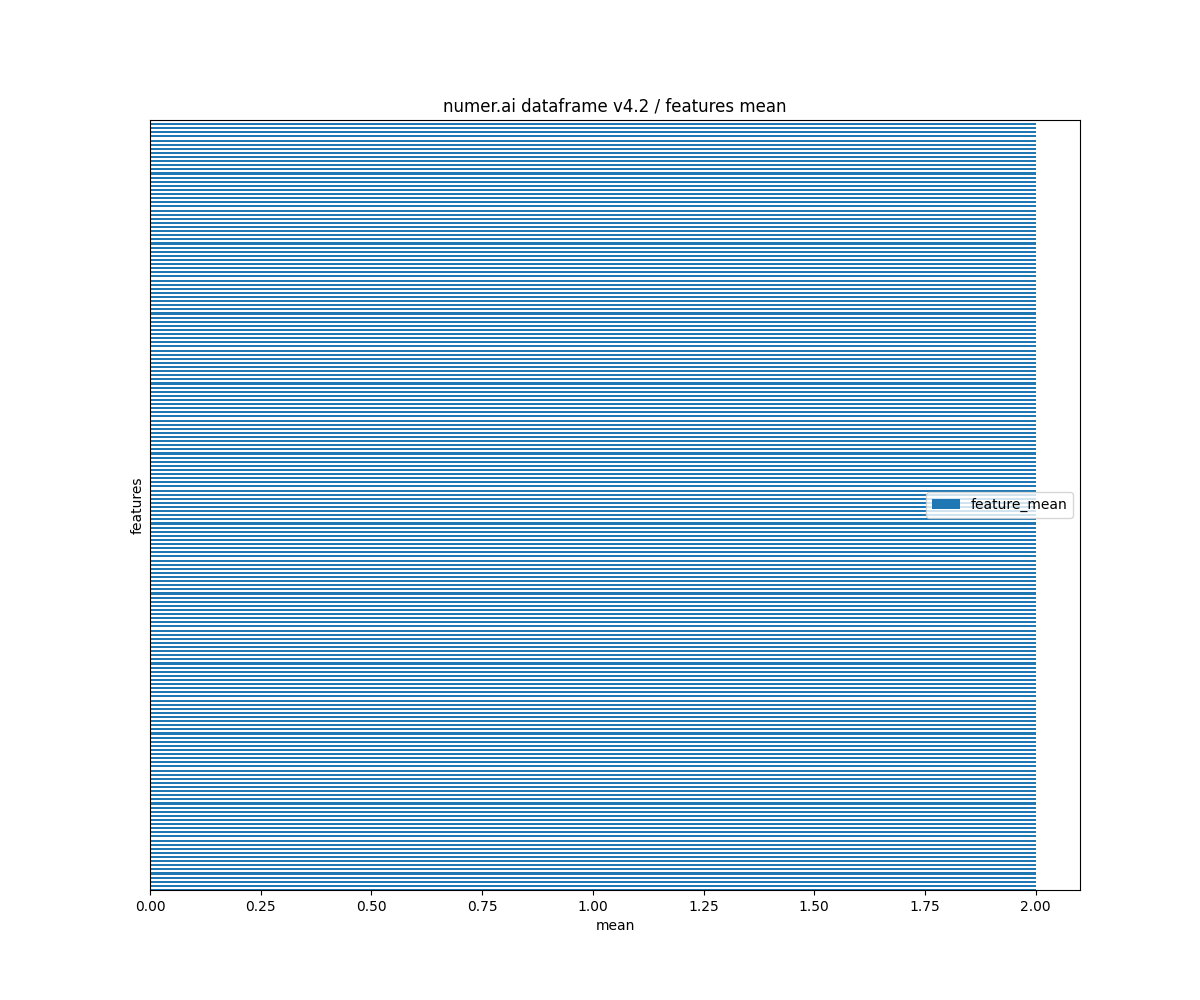
\includegraphics[width=1\textwidth,trim={0 0 0 0},clip]{figures/train_df_features_mean_horizontal_barplot_2023-09-30.png}
\caption[Mean of Features]{Mean $\mu$ of features $\vec{x}_i$} 
\label{fig: features_mean}  
\end{minipage}
\hfill
\begin{minipage}[t]{7cm}
\vspace{0pt}
\centering
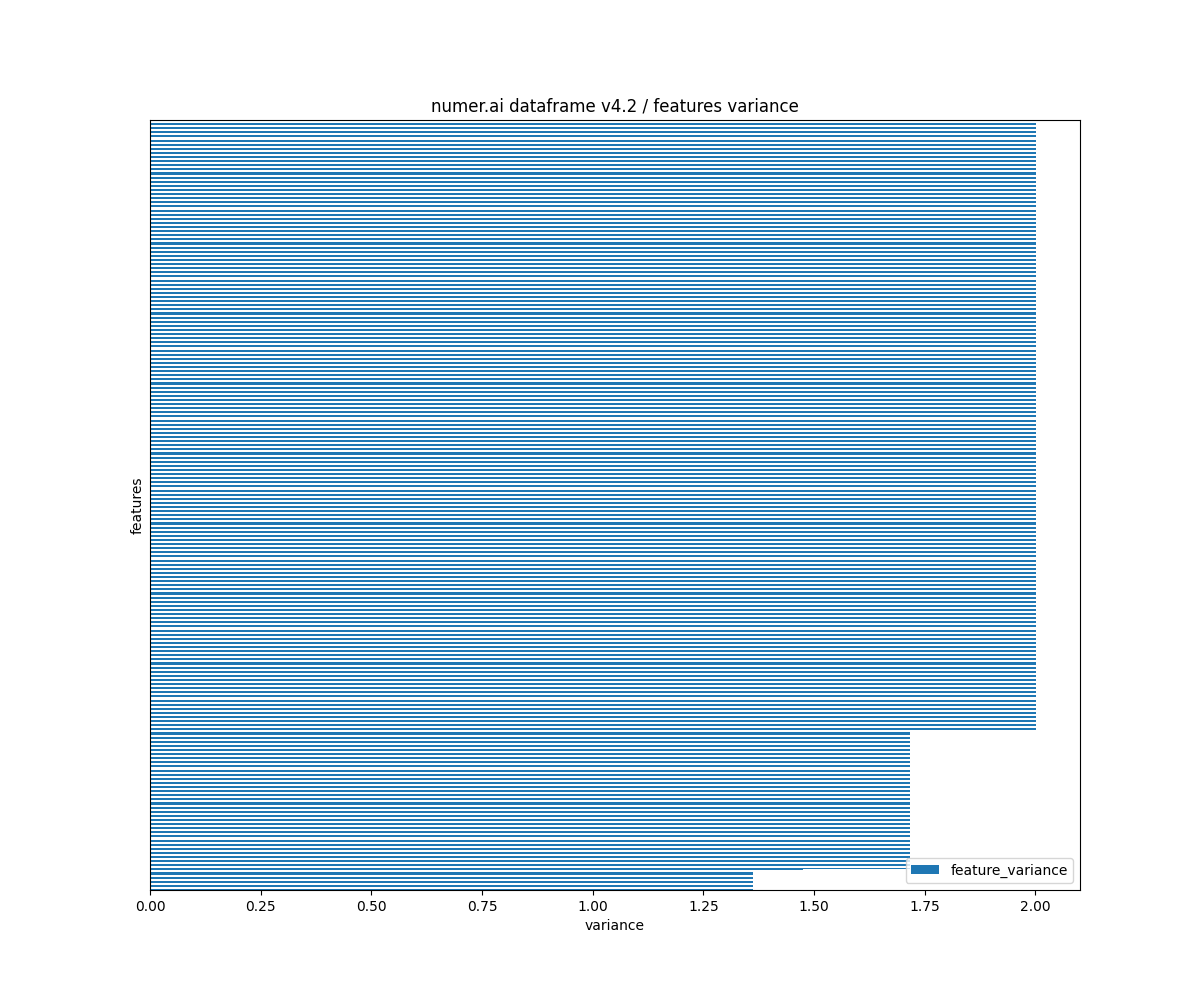
\includegraphics[width=1\textwidth,trim={0 0 0 0},clip]{figures/train_df_features_variance_horizontal_barplot_2023-09-30.png}
\caption[Variance of Features]{Variance $\nu$ of features $\vec{x}_i$ }
\label{fig: features_variance} 
\end{minipage}
\end{figure}
From the following plots one can obtain that through the induced variance of the features the distribution will not be uniform. Switching to the target room one get similar results. The provided targets are binned to $y_i \in [0,1]$ with a mean of $\mu(y) \approx 0,5$ [Fig. \ref{fig: targets_mean}] and most of the targets ($>$ 80 \%) have variance of $\nu(y) \approx 0,05$ [Fig. \ref{fig: targets_variance}].
\begin{figure}[htbp]
\begin{minipage}[t]{7cm}
\vspace{0pt}
\centering
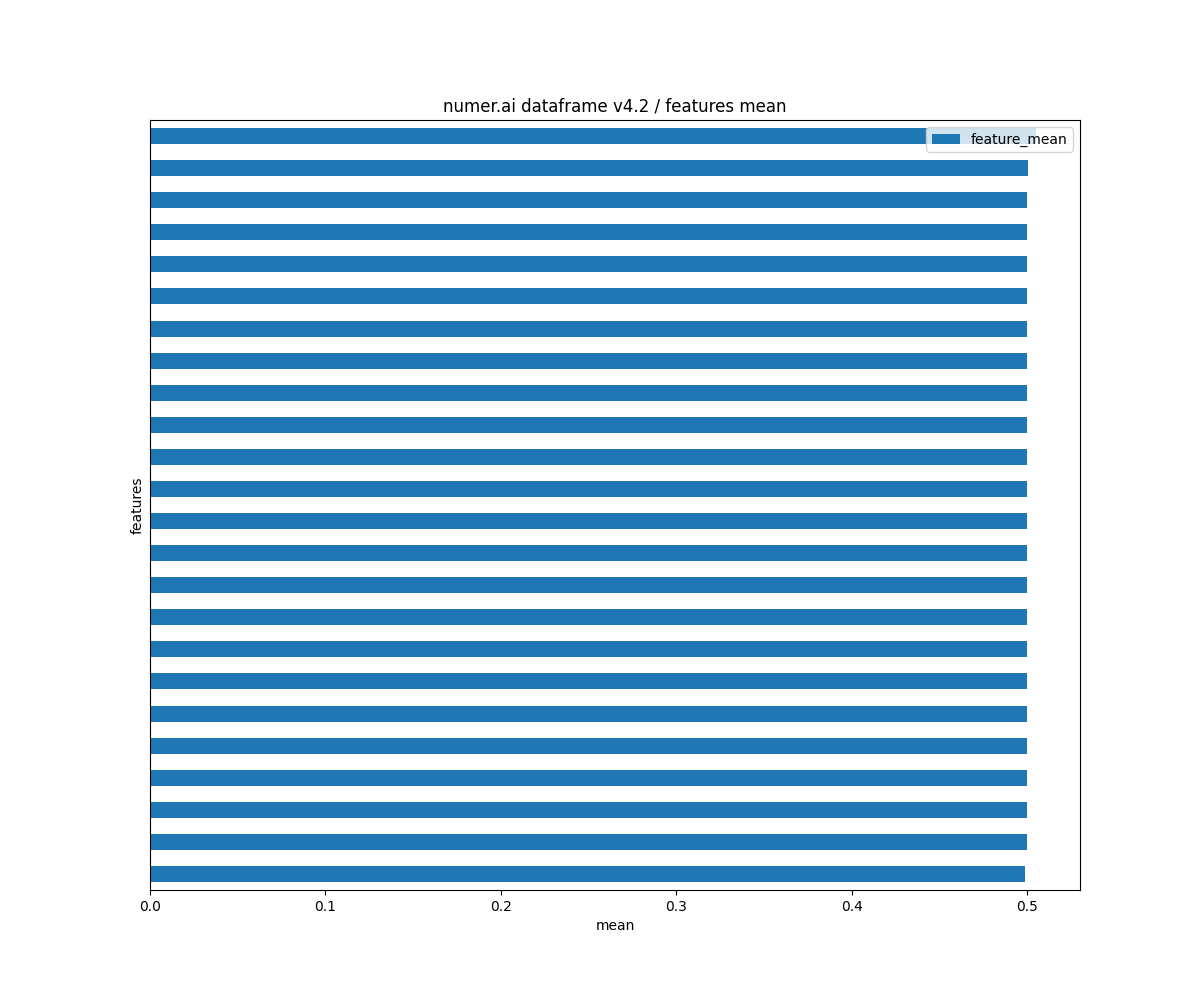
\includegraphics[width=1\textwidth,trim={0 0 0 0},clip]{figures/targets_df_targets_mean_horizontal_barplot_2023-09-30.png}
\caption[Mean of Targets]{Mean $\mu$ of targets $y_i$} 
\label{fig: targets_mean}  
\end{minipage}
\hfill
\begin{minipage}[t]{7cm}
\vspace{0pt}
\centering
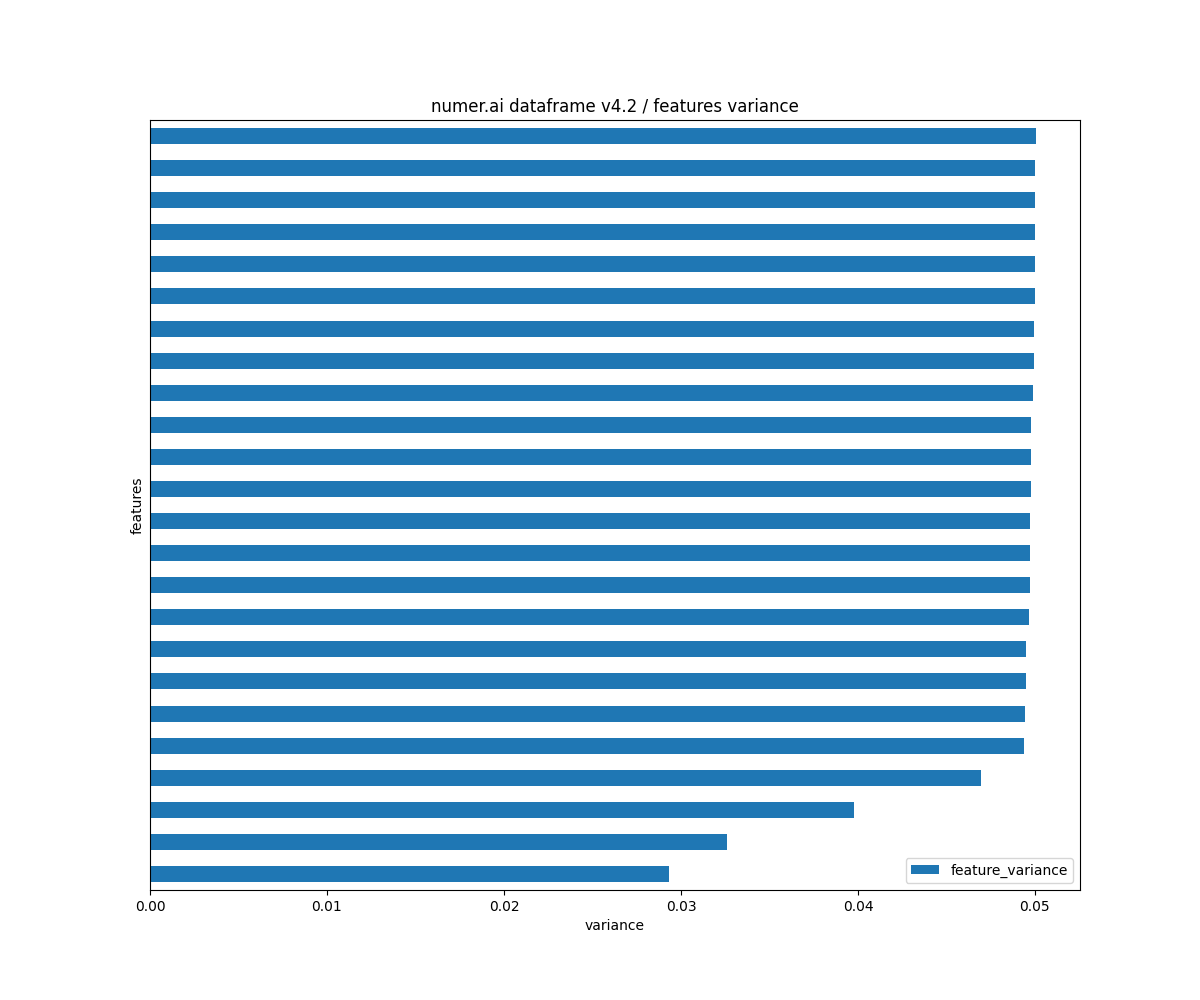
\includegraphics[width=1\textwidth,trim={0 0 0 0},clip]{figures/targets_df_targets_variance_horizontal_barplot_2023-09-30.png}
\caption[Variance of Features]{Variance $\nu$ of targets $y_i$ }
\label{fig: targets_variance} 
\end{minipage}
\end{figure}
%%%%%%%%%%%%%%%%%%%%%%%%%%%%%%%%%%%%%%%%%%%%%%%%%%%%%%%%%%%%%%%%%%%%%
\newpage
\subsection{Correlation maps of features and targets}
The correlation matrix of the features show that some features are indeed heavily correlated and some not [Fig. \ref{fig: numerai_features_correlation_matrix}]. Therefore it can make sense to exclude heavily correlated features in the beginning. But because of the additive modeling schematic over different base learners one get immediately the induced weights of informative versus informative features.
Interesting to note are recurrent patterns in the correlation matrix which results from the feature groups (quantitative features from a similar pot).
\begin{figure}[!htpb]
    \centering
    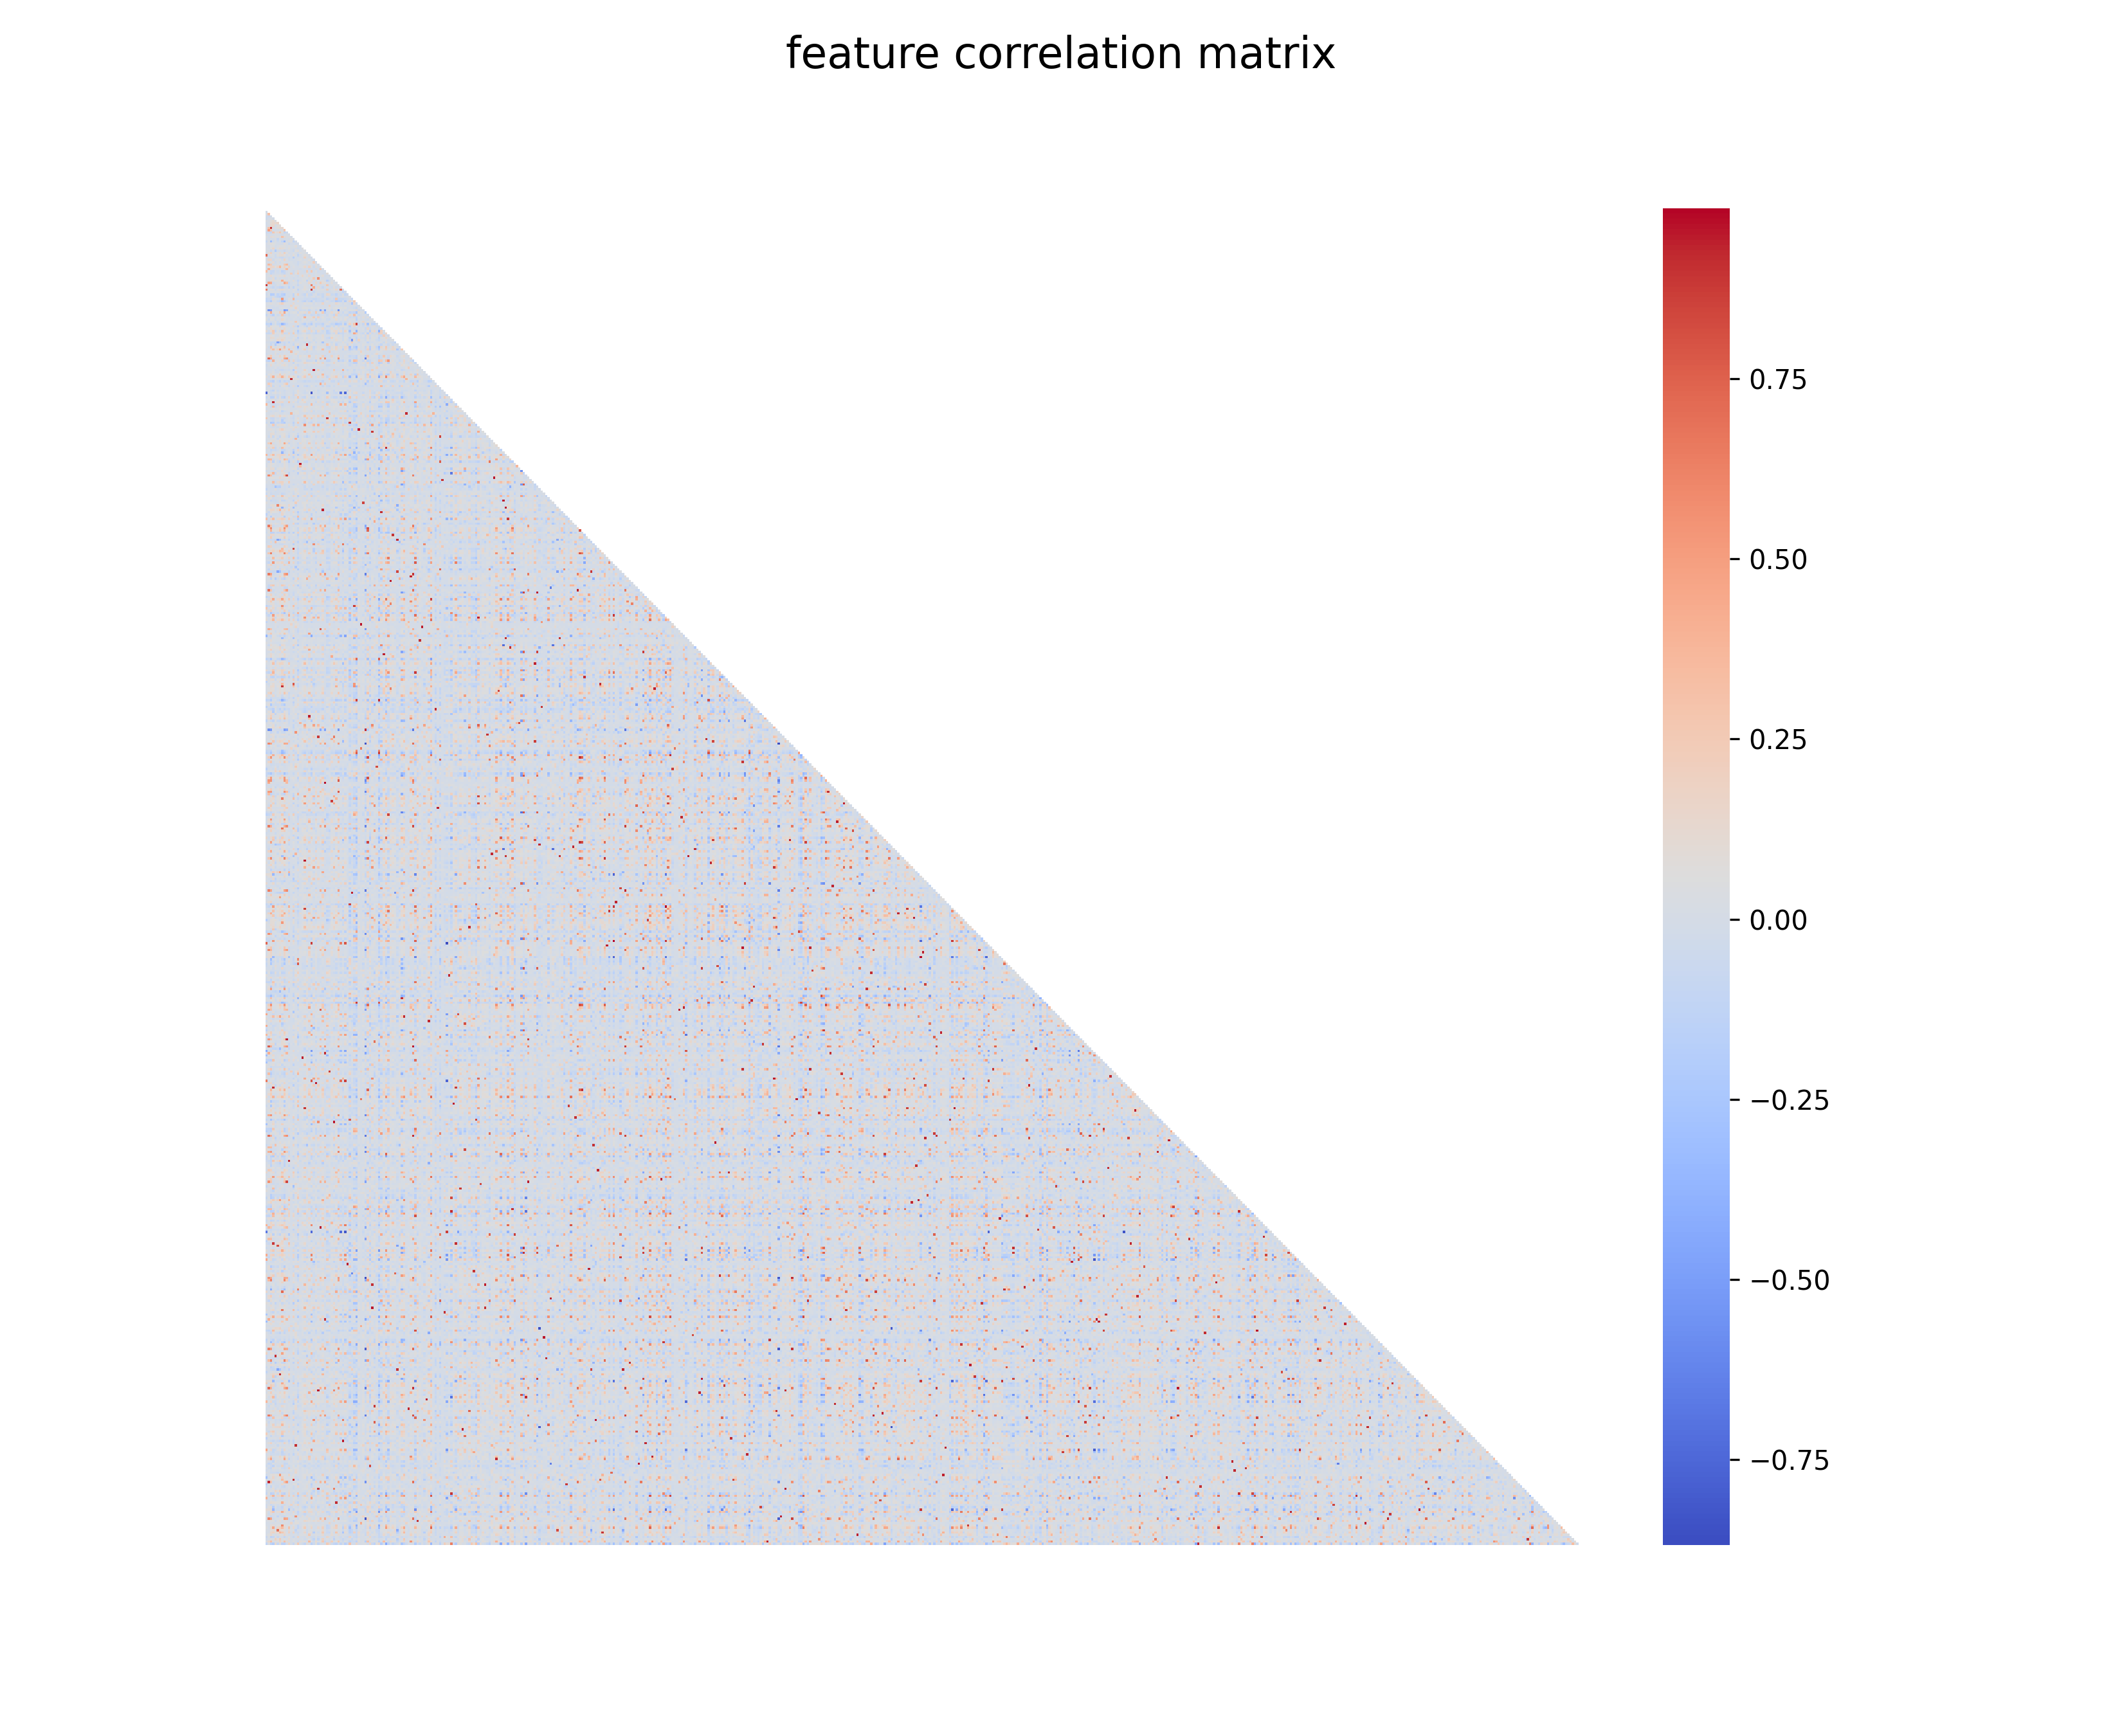
\includegraphics[width=0.8\textwidth,trim={0 0 0 0},clip]{figures/feature_correlations_matrix_2023-09-28.png}
    \caption[Numer.ai dataset features correlation matrix]{Numer.ai dataset features correlation matrix}
    \label{fig: numerai_features_correlation_matrix}    
\end{figure}
The correlation matrix of the targets also provides an insight for building the right ensemble model [Fig. \ref{fig: numerai_targets_correlation_matrix}]. Less correlated targets can indeed be useful for diversifying the prediction model in terms of feature exposure. Consequently the weights of the model will be distributed differently because of other feature importances. We'll use this for building an ensemble model to combine multiple model behaviors and to reduce risk. 
\begin{figure}[!htpb]
    \centering
    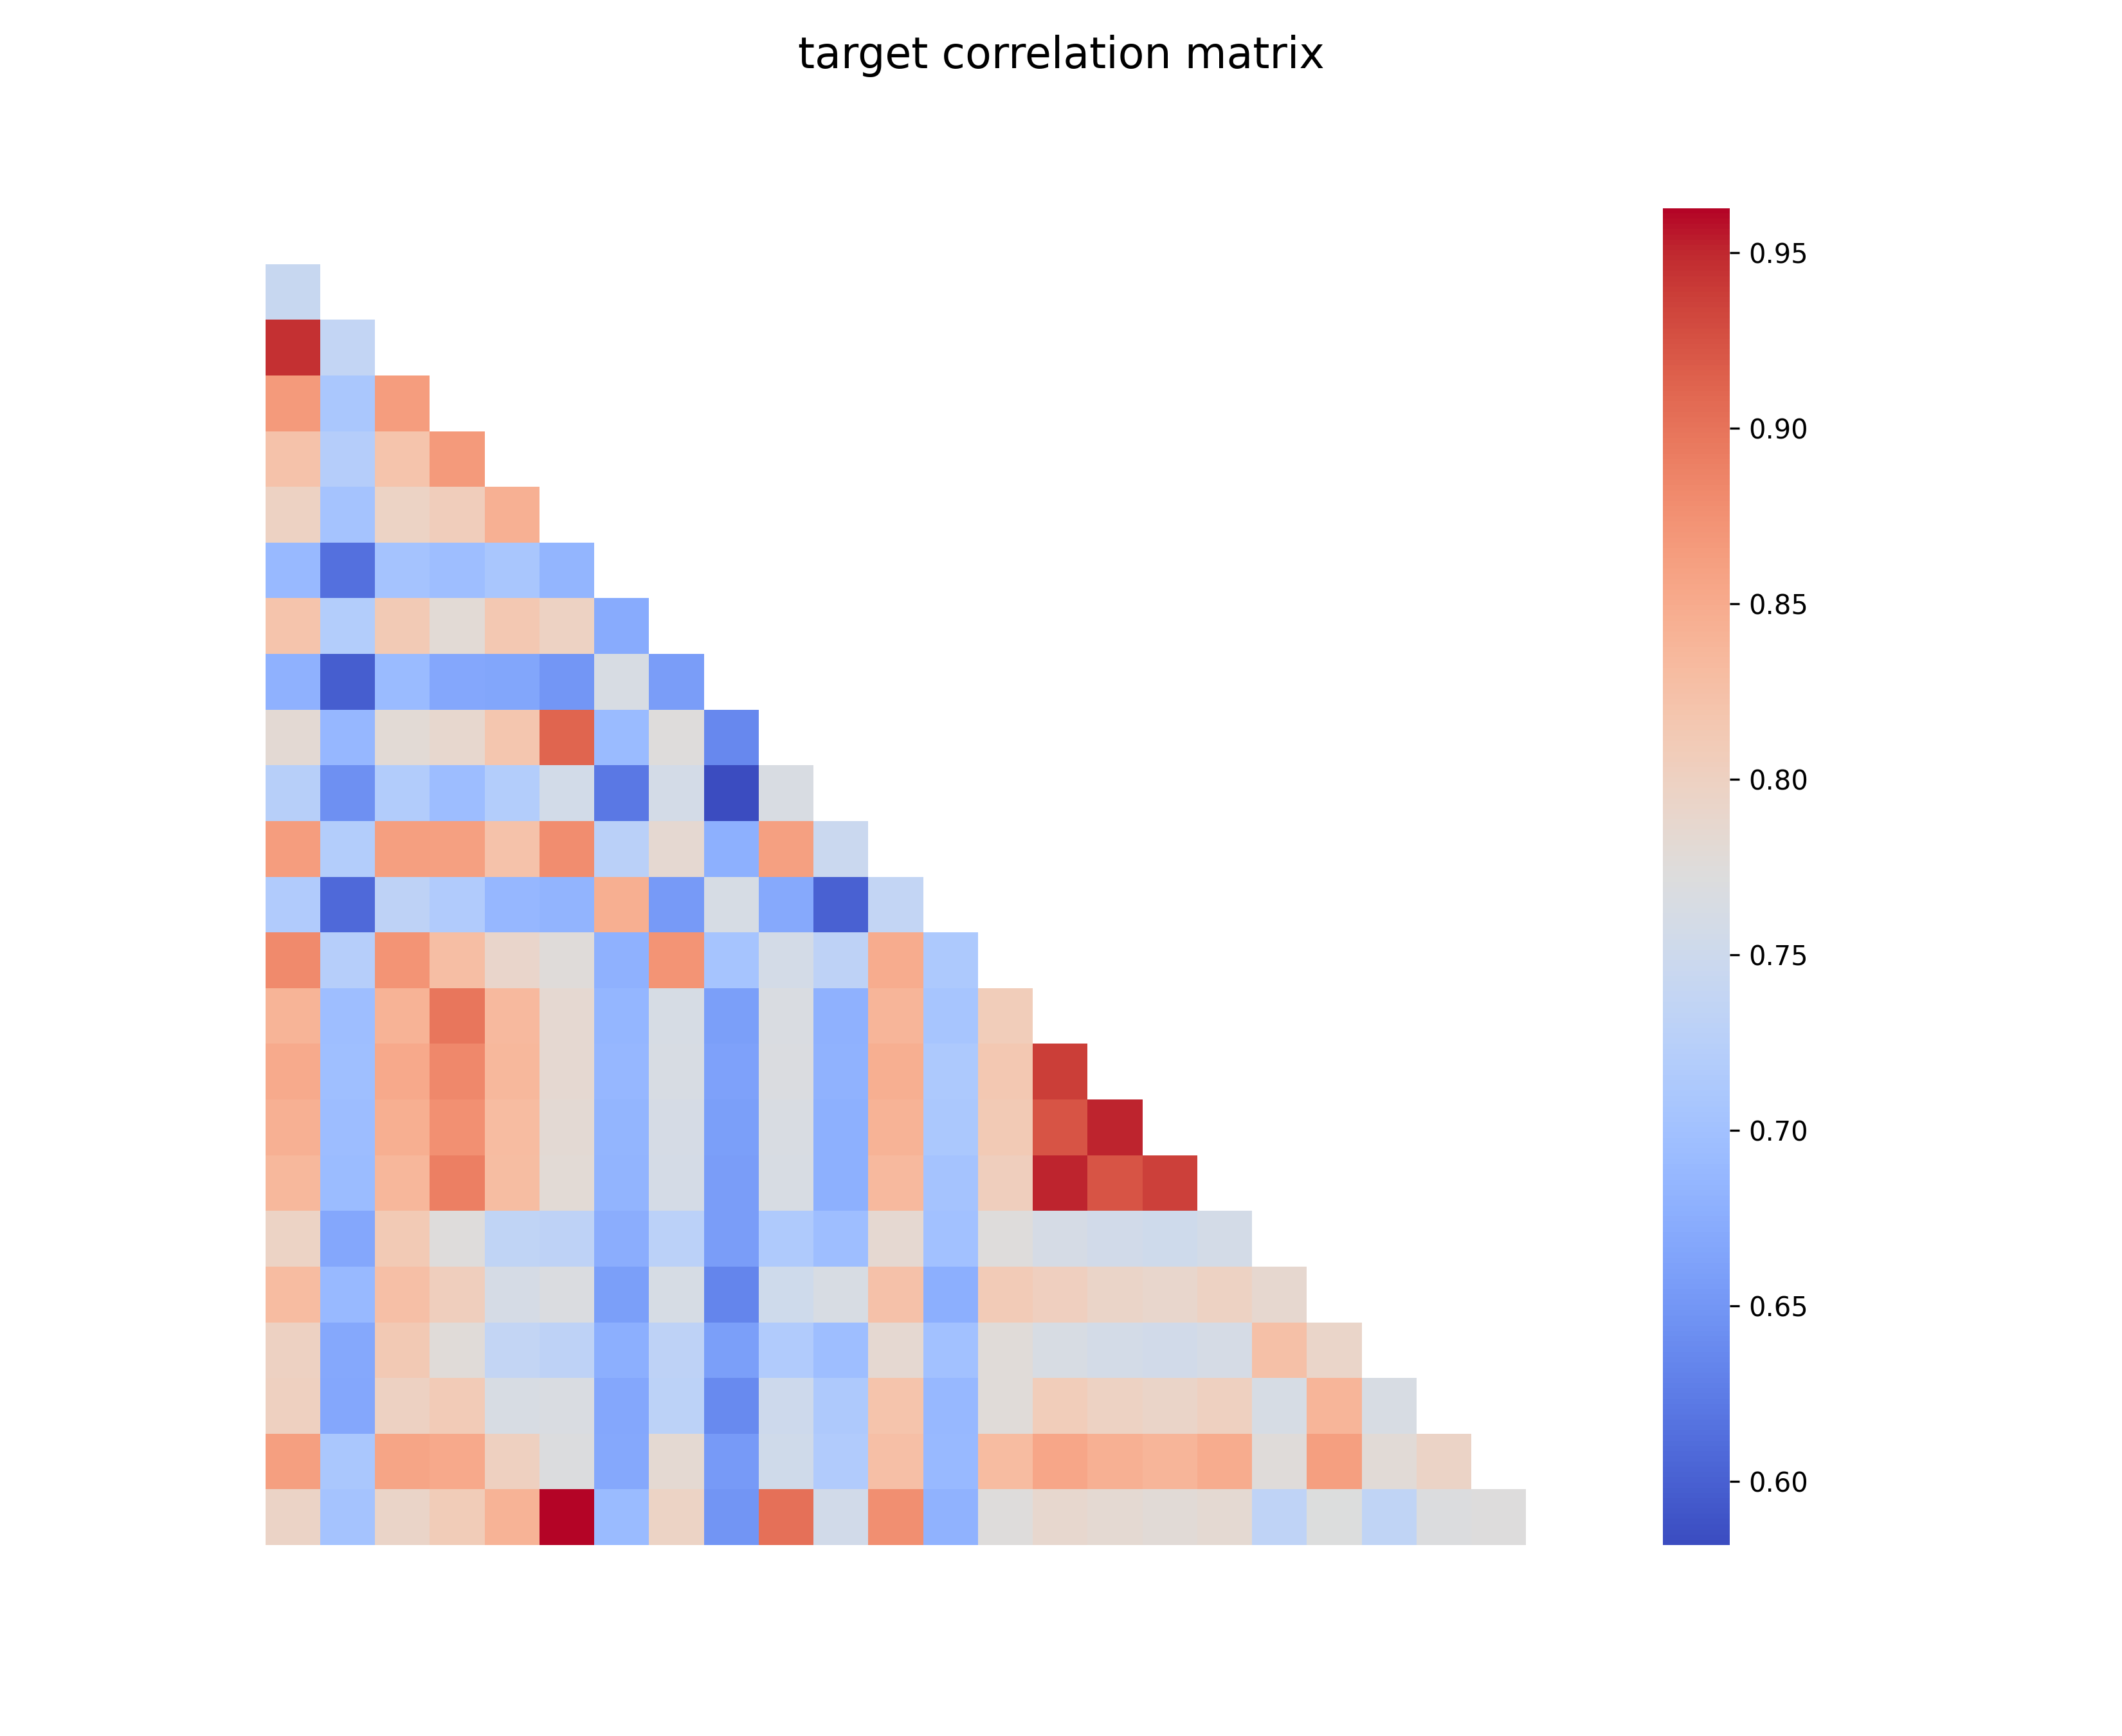
\includegraphics[width=0.8\textwidth,trim={0 0 0 0},clip]{figures/target_correlations_matrix_2023-09-28.png}
    \caption[Numer.ai dataset targets correlation matrix]{Numer.ai dataset targets correlation matrix}
    \label{fig: numerai_targets_correlation_matrix}    
\end{figure}
%%%%%%%%%%%%%%%%%%%%%%%%%%%%%%%%%%%%%%%%%%%%%%%%%%%%%%%%%%
\newpage
\subsection{Cross validation methods}
Because of the importance of cross validation at supervised machine learning tasks we've to compare different methods for validating our model performance. 
We'll use therefore the model selection method from the \href{https://scikit-learn.org/stable/modules/generated/sklearn.model_selection.KFold.html}{SKLEARN} python library. We'll use the classical $k$-fold cross-validation method ($k$ = 5) as explained in section [\ref{sec: cross_validation}]. In the framework there's the possibility to use different sub-methods whereby we'll focus on 4 different strategies:
\begin{itemize}
    \item $5$-fold with No Shuffling and No Random States
    \item $5$-fold with Shuffling and No Random States
    \item $5$-Grouped-fold with Shuffling and No Random States
    \item $5$-splitted TimeSeries Groups
\end{itemize}
Whereby the TimeSeries cross validation method is slightly modified compard to the Scikit's module, because it has to use groups and respect the era boundaries [\href{https://numer.ai}{numer.ai}].
When comparing this four different CV-methods by the standard score metric ($L_2$) one get slightly different values:
\begin{itemize}
    \item $5$-fold with No Shuffling and No Random States: $CV_{score} \approx 0,051$
    \item $5$-fold with Shuffling and No Random States: $CV_{score} \approx 0,054$
    \item $5$-Grouped-fold with Shuffling and No Random States: $CV_{score} \approx 0,052$
    \item $5$-splitted TimeSeries Groups $CV_{score} \approx 0,045$
\end{itemize}
One would possibly think when dealing with a TimeSeries-dataset that consequently the Time-Series-Split would result in the best score. The Time-Series-Split is a variation of $k$-fold which returns first $k$-fold as train-set and the $(k + 1)$-th fold for testing [Ref. \href{https://scikit-learn.org/stable/modules/cross_validation.html#k-fold}{Scikit}]. But we can obtain that with $k$-fold Cross-Validation ($k$ = 5) with Shuffling one gets the best score on the dataset prediction. Therefore we'll use this metric for evaluation.
%%%%%%%%%%%%%%%%%%%%%%%%%%%%%%%%%%%%%%%%%%%%%%%%%%%%%%%%%%%%%%%
\subsection{Hyperparameter selection and optimization}
With the Bayesian Optimizer we'll try to predict based on the best cross-validation metric the best hyperparameter combination as described in section [\ref{sec: bayesian_opt_test}]. \\
Due to the size of the dataset the optimization process is computationally very expensive for a solid number of iterations. Because of limited hardware ressources we'll dimensionally reduce the dataset with PCA. The information $IL(\vec{x})$ which occurs is then proportional to the variance as descriped in section [\ref{sec: pca}]. \\
It will be assumed that the reduction process via PCA do not inherently change the modeling behavior and therefore the objective function will be retained. By reducing the 583 features (medium dataset) to $n = 300$ principal components the information loss results in $IL(\vec{x}) \approx 0,044 \%$. After reducing the dataset the \href{https://github.com/bayesian-optimization/BayesianOptimization}{Bayesian Optimizer framework} will be used with Upper-Confidence-Bounds acquisition function (standard method in the used module) and $n_{iter} = 100$ iterations and $init_{points} = 10$ points for exploration. \\
We'll use the same hyperparameter constellation as in the test-case problem but with slightly larger parameter domains because of the huge dataset:
\begin{itemize}
    \item Learning Rate $\nu \in  [0,01 ; 0,2]$
    \item Maximal depth of trees $d_{max} \in [1; 10]$
    \item Number of Trees $n_{trees} \in [100; 30000]$
    \item Colsample by Tree $\epsilon \in [0,1; 1]$
\end{itemize}
The resulting constellation of hyperparameter-values which maximizes our objective function best possible over the training's-dataset with $5$-fold-CV are: \\
\begin{center}
    Learning Rate $\nu = 0,02$ / Maximal depth of trees $d_{max} = 2$ \\ Number of Trees $n_{trees} = 2465$ / Colsample by Tree $\epsilon = 0,2$
\end{center}
(The runtime for the Bayesian Optimization task takes around 70 hours with the stated hardware.)
%%%%%%%%%%%%%%%%%%%%%%%%%%%%%%%%%%%%%%%%%%%%
\subsection{Ensemble modeling}
For building an ensemble model $F_E(\vec{x})$ one has to evaluate the specific properties of every sub-model $F_i(\vec{x})$. Because of computational efficiency we'll use the \href{https://lightgbm.readthedocs.io/en/stable/}{LightGBM} framework for modeling instead of the self written algorithm [\href{https://github.com/probabilis/bs_ml}{Github Repository}], but ultimately the underlying clockwork of the \textit{Gradient Boosting}-Framework with \textit{Decision Tree}-Regressor as base learners is identical. One has to mention that because of the huge development of the framework there's always the possibility to configure the base model or add additional hyperparameters.\\
With the given prediction problem we've the possibility to train each model versus a different target value which are correlated at different scale. The main target which is used to calculate the model performance is currently \textit{target cyrus}. Evaluating the model performance over all different targets results in a very solid performance of \textit{target nomi} and  \textit{target victor}. \\
Because one wants to reduce overall risk of the model to specific feature exposures we'll add an additional target which do not have ultimately the best performance but rather the least correlation to the main target. Through comparing all of the correlation values in the correlation matrix of the given targets one can calculate the least correlated target: \textit{target alan}. Summing up we'll use following targets, which describe 20-day stock market returns, to create the ensemble model: \\
\begin{itemize}
    \item \textit{target cyrus} (main target) 
    \item \textit{target nomi}
    \item \textit{target victor}
    \item \textit{target alan}
\end{itemize}
The weights $\omega_i(\vec{x})$ of the model combination we'll be set equally for simplification. One can optimize this by searching the right weights also by Bayesian Optimization. \\ 
Additionally the predictions have to be ranked by percentile ($PR[\cdot]$) for normalization ($\tilde{y} \in$ [0,1]) to be compatible for submission.
\begin{center}
    $\tilde{y} = PR[F_E(\vec{x})] = PR[\sum_{i=1}^{N=4} \omega_i(\vec{x}) F_i] \quad$ with $\omega_i(\vec{x}) = \omega = 1/4$ 
\end{center}
%%%%%%%%%%%%%%%%%%%%%%%%%%%%%%%%%%%%%%%%%%%%%%%%%%%%%%%%%%%%%%%%%%%
\subsection{Neutralizing}
\label{sec: neutralizing}
When predicting stochastically behaving systems like the stock market it's very tough to treat this ``non-stationary`` relationship between features and returns. Features that have strong predictive power during some periods may not have any in other time periods or may even completely reverse. This specific uncertainty is what is called ``feature risk``. We can evaluate from the dataset that they're single features with have an in-depth correlation with the target over time (eras). When calculating the individual features exposures, which is a measurement of the Pearson correlation between a model's predictions and each feature, one can obtain that the model is indeed highly correlated to some specific features [Fig. \ref{fig: per_era_correlation}], whereby similar features got grouped together by Numer.ai (in total 8 groups). 
\begin{figure}[!htpb]
    \centering
    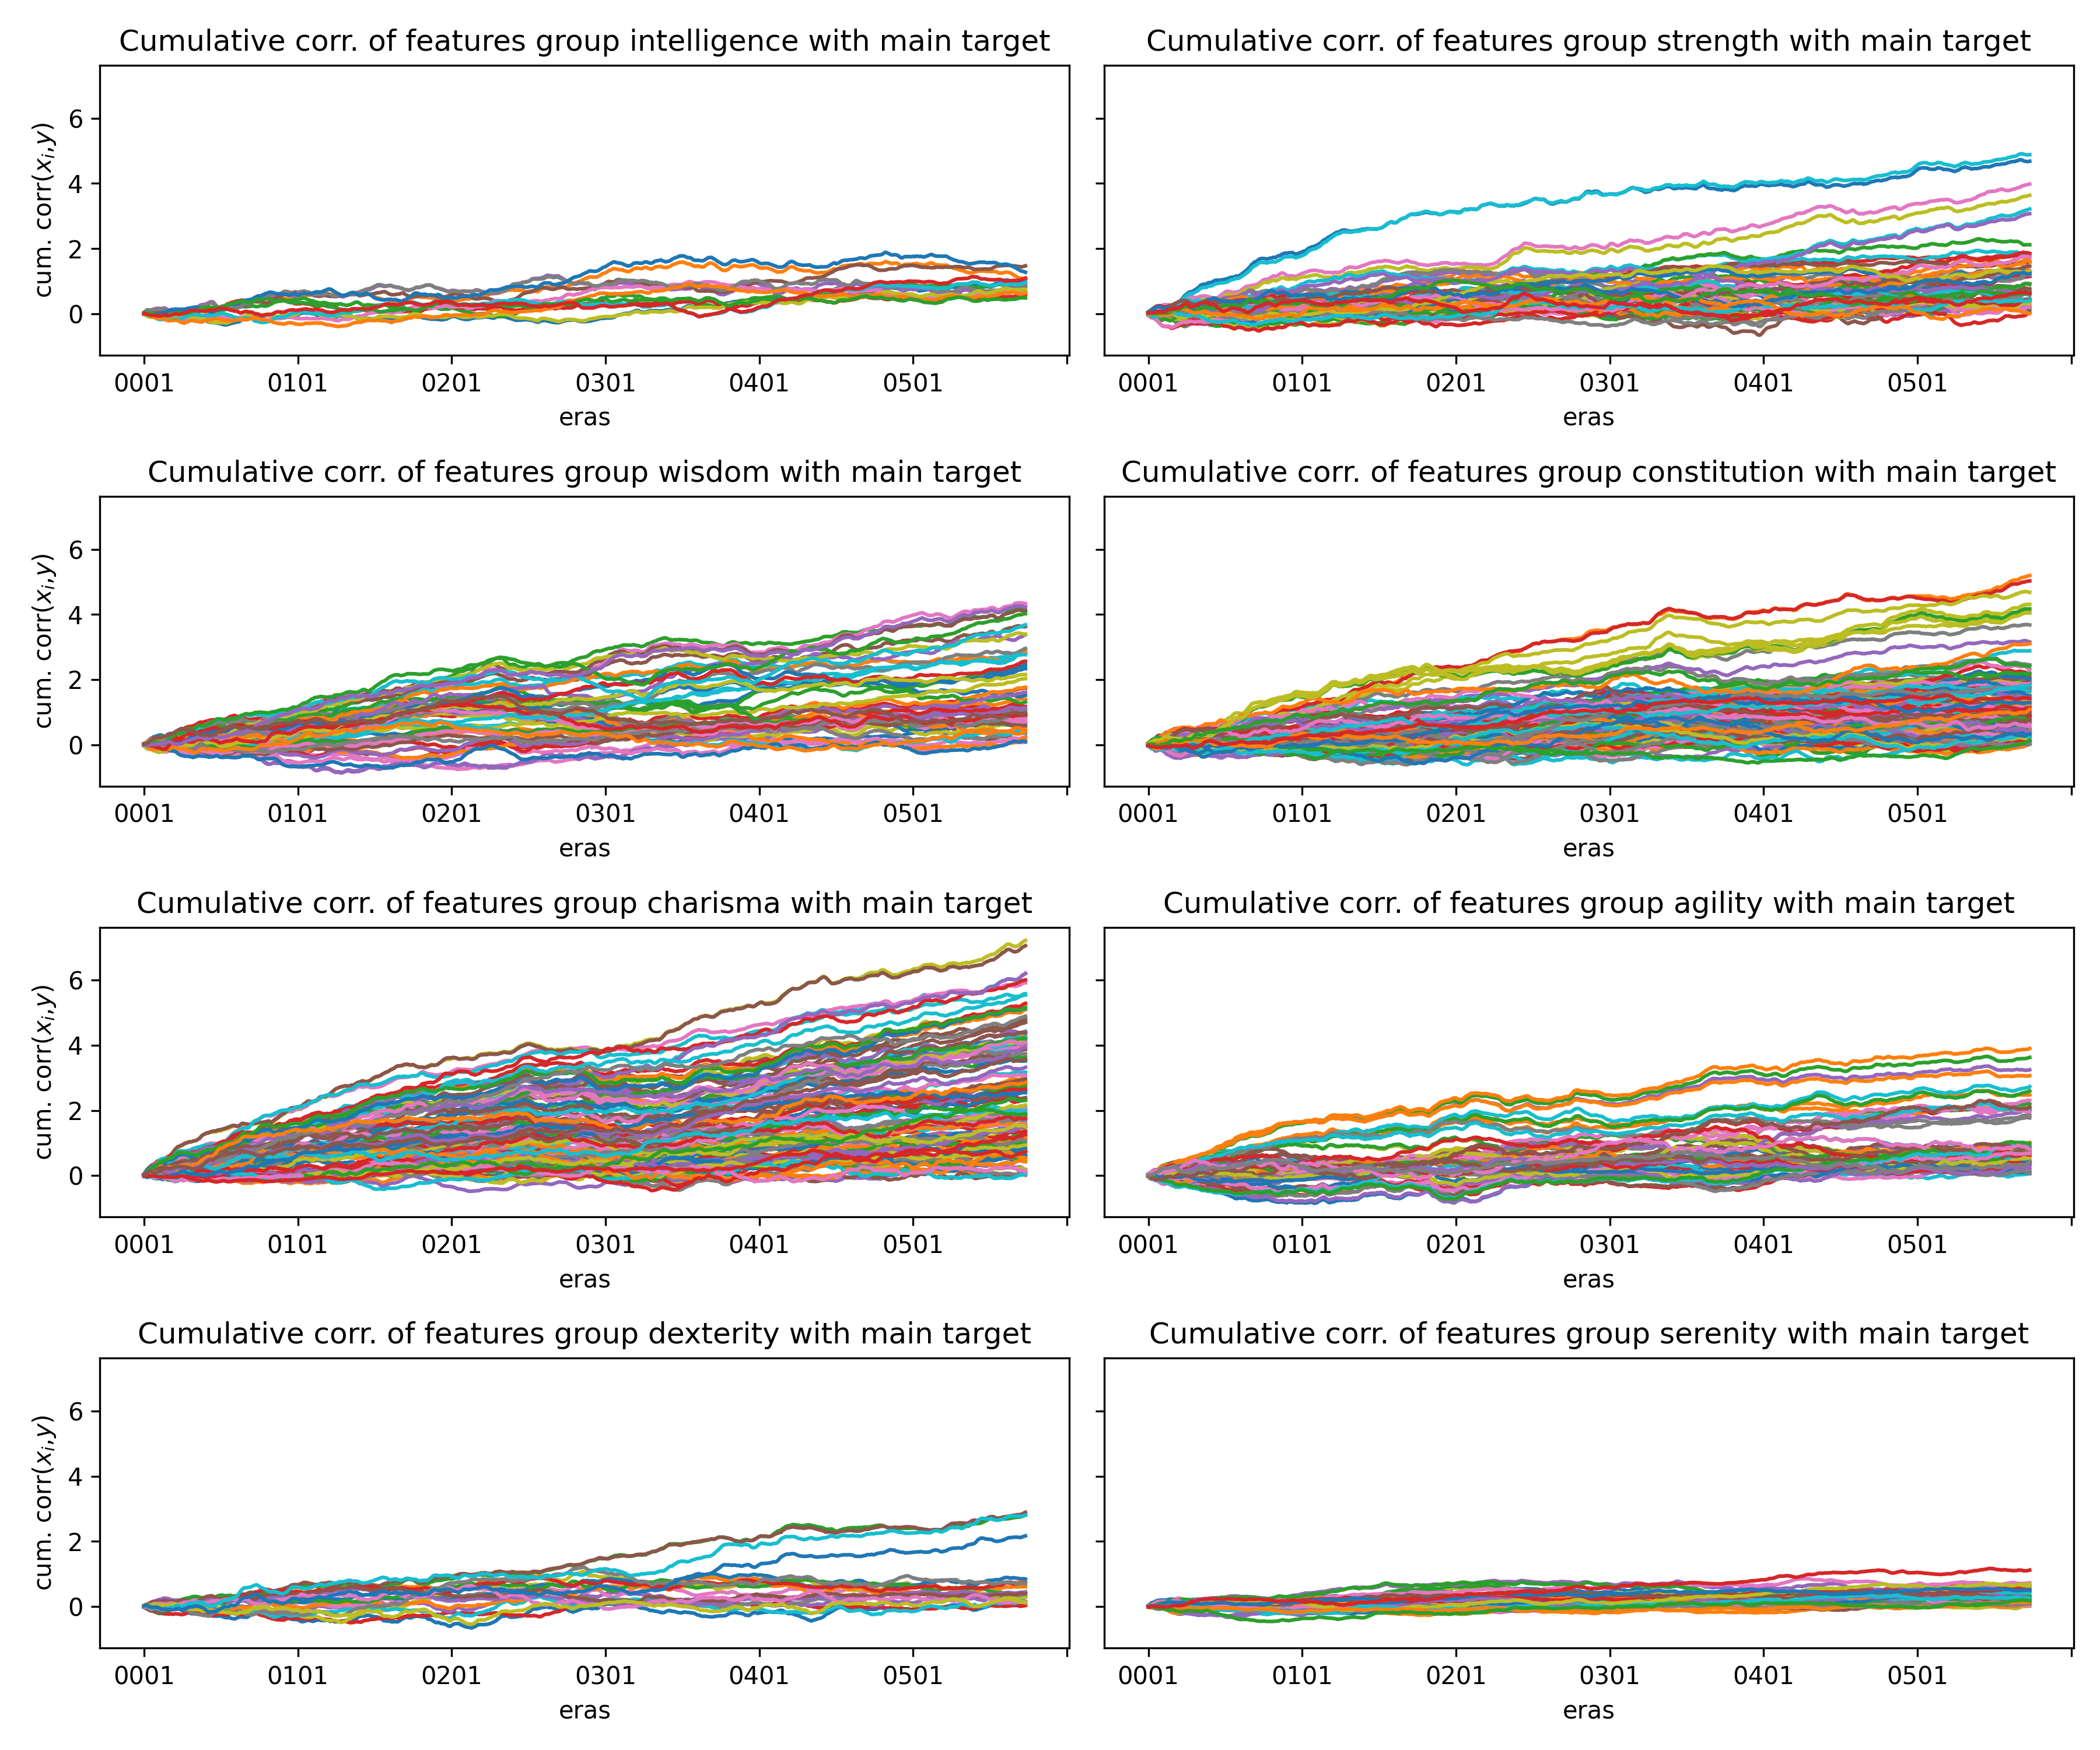
\includegraphics[width=1\textwidth,trim={0 0 0 0},clip]{figures/per_era_correlations.png}
    \caption[Cumulative per era correlation of the different feature groups]{Cumulative per era correlation of the different feature groups over the main \textit{target cyrus}}
    \label{fig: per_era_correlation}    
\end{figure}
Therefore one can use ``Feature Neutralization`` to reduce feature exposure. This process, at a high level, is nothing more than removing the component of the predictions that are linearly correlated with certain features, leaving only the residual non-linear component [Ref. \href{https://forum.numer.ai/t/an-introduction-to-feature-neutralization-exposure/4955}{Numer.ai}]. When reducing only one feature $x_1$ for simplicity the following consideration has to take place. Without loss of generality, one can assume that the true target value $y$ is determined by the following function:
\begin{equation}
\label{eq: neutral_x1}
    y = f(x_1) + g(x_1, x_2,...)
\end{equation}
Whereby the component $f(x_1)$ only contributes $x_1$ to $y$. Under the assumption of ignoring terms above the seconder order, the neutralization for $x_1$ is equivalent to deleting $f(x_1)$. This result can be obtained through a calculation to find $\alpha$ and $\beta$ that minimize the squared error of equation (\ref{eq: neutral_x1}): $\alpha x_1 + \beta$.
Because it is only a first-order approximation, this argument does not hold if the absolute value of the feature value is large.
In order to do this, \href{https://forum.numer.ai/t/an-introduction-to-feature-neutralization-exposure/4955}{Numer.ai} propose using the \textit{Moore Penrose matrix} for finding a matrix's inverse. As the matrix which has to be inverted has more rows that columns it is not invertible per se, with Moore Penrose's inverse we find the pseudoinverse that minimizes least-squared error. So for the feature neutralization process one has to take the whole dataframe, where the columns have to be neutralized and the neutralization proportion as input. 
\[  
\begin{bmatrix}  
a_{11} & a_{12} & .. & .. \\  
a_{21} & a_{22} & .. & .. \\  
.. & .. & .. & .. \\  
.. & .. & .. & a_{mn} \\  
\end{bmatrix}  
\begin{bmatrix}  
x_1 \\  
.. \\  
.. \\  
x_n \\  
\end{bmatrix}  
=
\begin{bmatrix}  
y_1 \\
.. \\  
.. \\  
y_n \\  
\end{bmatrix}  
\text{where} \quad m > n \quad \text{or} \quad \hat{A} \vec{x} = \vec{y} \]
Whereby the vector $\vec{y}$ can be thought of as the scores and $\vec{x}$ can be thought of as a vector of $\beta$-values. The Penrose-Matrix gets denoted as $\hat{A}^{mp}$ and one gets:
\begin{equation}
    \hat{A} \hat{A}^{mp} \vec{x} \approx \hat{A}^{mp} \vec{y} \rightarrow I \vec{x} \approx \hat{A}^{mp} \vec{y} \rightarrow \hat{A}^{mp} \approx (\hat{A}^T \hat{A}^{-1}) \hat{A}^T 
\end{equation}
and this results to $\vec{x} \approx \hat{A}^{mp} \vec{y}$, which produces a solution with the least squared error and this is why one can think of the $\vec{x}$-vector as a $\beta$-vector where each $\beta$- represents the coefficients of a least squares linear solution. This prediction is then multiplied by the desired proportion and subtracted from the original score vector to create a new one. Finally the new score vector is divided by its standard deviation to rescale it and the reduction of feature exposure is completed. This results in a trade-off between neutralization (which increases consistency in predictions) and correlation [Fig. \ref{fig: feature_neutral}].
\begin{figure}[!htpb]
    \centering
    \includegraphics[width=0.5\textwidth,trim={0 50 0 0},clip]{figures/feature_neutralization.png}
    \caption[Feature neutralization trade-off]{Feature neutralization trade-off between consistency and correlation from \href{https://forum.numer.ai/t/an-introduction-to-feature-neutralization-exposure/4955}{Numer.ai}}
    \label{fig: feature_neutral}    
\end{figure}
%%%%%%%%%%%%%%%%%%%%%%%%%%%%%%%%%%%%%%%%%%%%%%%%%%%%%
\newpage
\subsection{Scoring methods}
For evaluating the scores of our models one can use different metrics. The standard process would be to use the correlation from the calculated predictions $\hat{y}$ with the provided target values $y$. But because we're dealing with a dataframe from the financial markets we can introduce two additional performance metrics like ``sharpe``-ratio and ``maximal drawdown``. The sharpe ratio measures the performance of an investment $R_a$ compared to a risk-free asset $R_b$, after adjusting for its risk.
\begin{equation}
    \label{eq: sharpe_ratio}
    S_a = \frac{\mathbb{E}[R_a - R_b]}{\sigma_a}
\end{equation}
The maximum drawdown is the maximum observed loss from a peak over the history of the variable, before a new peak is attained. So it indicates downside risk over a specified time period.
\begin{equation}
\label{eq: mdd}
    MDD = \underset{\tau \in (0,T)}{\max} D(\tau) =  \underset{\tau \in (0,T)}{\max} [ \underset{t \in (0,\tau)}{\max} X(t) - X(\tau)]
\end{equation}
In addition there's a predefined correlation function $C_{nmr}$ written by \href{https://docs.numer.ai/numerai-tournament/scoring/correlation-corr}{Numer.ai}, which is the primary scoring metric. It uses a special variation of correlation. At a high level, this metric is designed to be a good approximation for actual portfolio returns if the predictions were used in live trading. \\
%%%%%%%%%%%%%%%%%%%%%%%%%%%%%%%%%%%%%%%%%%%
\newpage
\section{Results and Model Interpretation}
Summing up again the ingredients which were needed to create a solid model and to participate in the data science prediction problem:
\begin{itemize}
    \item Gradient Boosting Machine based on Decision Trees
    \item 5-fold Cross Validation metric
    \item Bayesian Optimizer
    \item Selection metric for ensemble model
    \item Score metrics for evaluation
\end{itemize}
Through Bayesian Optimization the best hyperparameter combination via the CV metric will be evaluated which get fed into Gradient Boosting Machine based on Decision Trees as base learners. The model (shorthanded as GBM$^{\ast}$) will be trained on the \textit{training dataframe} via different targets and evaluated on the \textit{validation dataframe}. In the following summary table [Tab. \ref{table: summary_metric_predictions}] the mean of the predicted target values $\tilde{y}_i(\vec{x})$, the standard deviation of the predicted targets $\sigma_i(\vec{x})$, the sharpe ratio $S_i$ (\ref{eq: sharpe_ratio}) whereby the risk free yield is set to 0 \%, the maximum drawdown $MDD$ (\ref{eq: mdd}) and the mean correlation $C_{iCyrus}$ with \textit{target cyrus}, as it as the main target for prediction. 
\begin{table}[!htbp]
\centering
\caption{Summary metrics of prediction values from different targets \\
predicted target values $\tilde{y}_i(\vec{x})$ \\
standard deviation of the predicted targets $\sigma_i(\vec{x})$ \\
sharpe ratio $S_i$ (\ref{eq: sharpe_ratio}) with risk free yield 0 \% \\
maximum drawdown $MDD$ (\ref{eq: mdd}) \\
mean correlation $C_{iCyrus}$ with \textit{target cyrus} \\}
\label{table: summary_metric_predictions}
\begin{tabular}{|l|l|l|l|l|l|}
\hline
\textit{targets} & mean[$\tilde{y}_i(\vec{x})$] & $\sigma_i(\vec{x})$ & $S_i$ & $MDD$ & $C_{iCyrus}$ \\ \hline
\hline
\hline
\textit{cyrus} & 0,0191 & 0,0207 & 0,9214 & 0,0510 & 1,0  \\ \hline
\textit{alan} & 0,0107 & 0,0213 & 0,4995 & 0,1000 & 0,6650 \\ \hline
\textit{nomi} & 0,0191 & 0,0207 & 0,9217 & 0,0393 & 0,8248 \\ \hline
\textit{victor} & 0,0184 & 0,0187 & 0,9852 & 0,0456 &  0,8290 \\ \hline
\end{tabular}
\end{table}
%%%%%%%%%%%%%%%%%%%%%%%%%%%%%%%%%%%%%%%%%%%
We can obtain that beside the main \textit{target cyrus} the \textit{target victor} and \textit{nomi} result in nearly identical sharpe ratios over the validation dataframe whereby \textit{target alan} results in a very low sharpe ratio in comparison. The maximum drawdown is lowest on \textit{nomi} but highest on \textit{alan}. Which is a possible consequence of the fact that \textit{target alan} has the lowest correlation to \textit{target cyrus}. In the following figure [\ref{fig: cum_corr_val_preds}] the cumulative correlation of validation predictions is shown.
\begin{figure}[!htpb]
    \centering
    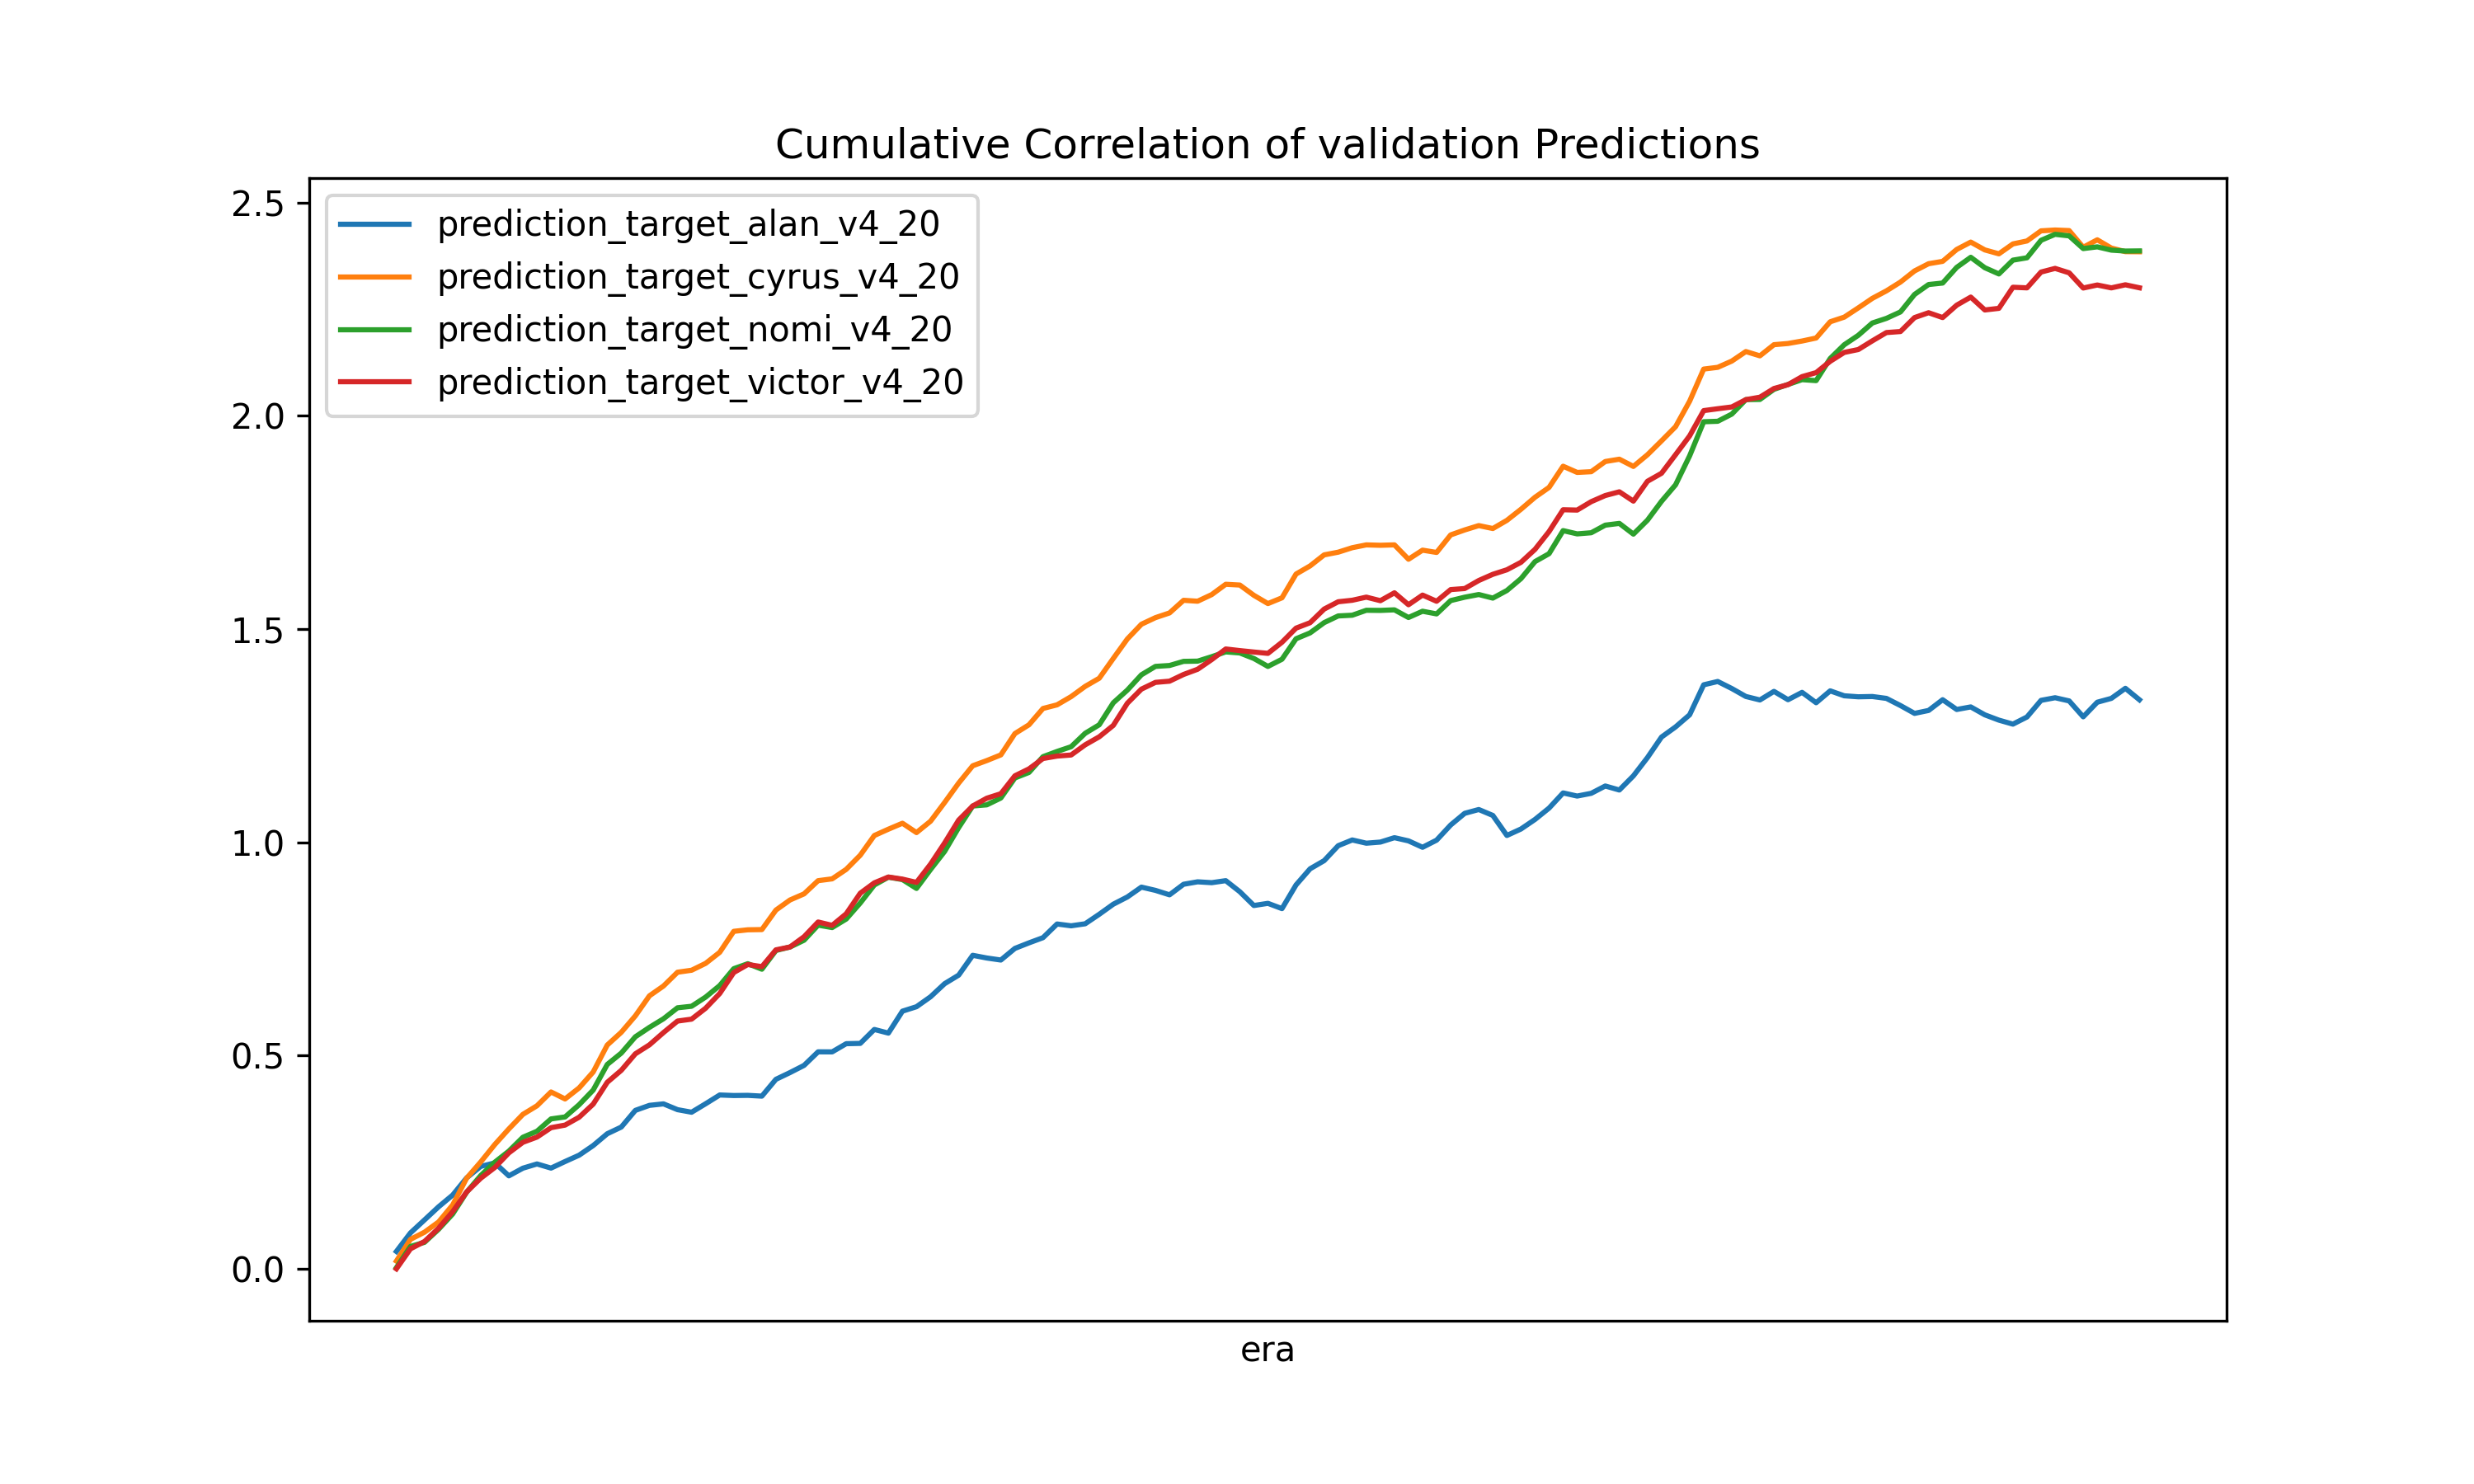
\includegraphics[width=1\textwidth,trim={0 0 0 0},clip]{figures/2023-09-28_round2_cumulative_correlation_of_validation_predicitions.png}
    \caption[Cumulative per era correlation of validation predictions over the GBM$^{\ast}$ models with different targets]{Cumulative per era correlation of validation predictions $\tilde{y}(\vec{x}(t))$ over the GBM$^{\ast}$ model with different targets $y(\vec{x}(t))$}
    \label{fig: cum_corr_val_preds}    
\end{figure}
The main \textit{target cyrus} performs consistently the best, whereby \textit{target alan} performs worst. Interesting to note is the peak correlation with followed sideway behavior. \\
Lastly we'll take a look on the feature importances (as stated in section [\ref{sec: decision_trees}]) of the sub-models [Fig. \ref{fig: fi_cyrus} - \ref{fig: fi_alan}].
\begin{figure}[htbp]
\begin{minipage}[t]{7cm}
\vspace{0pt}
\centering
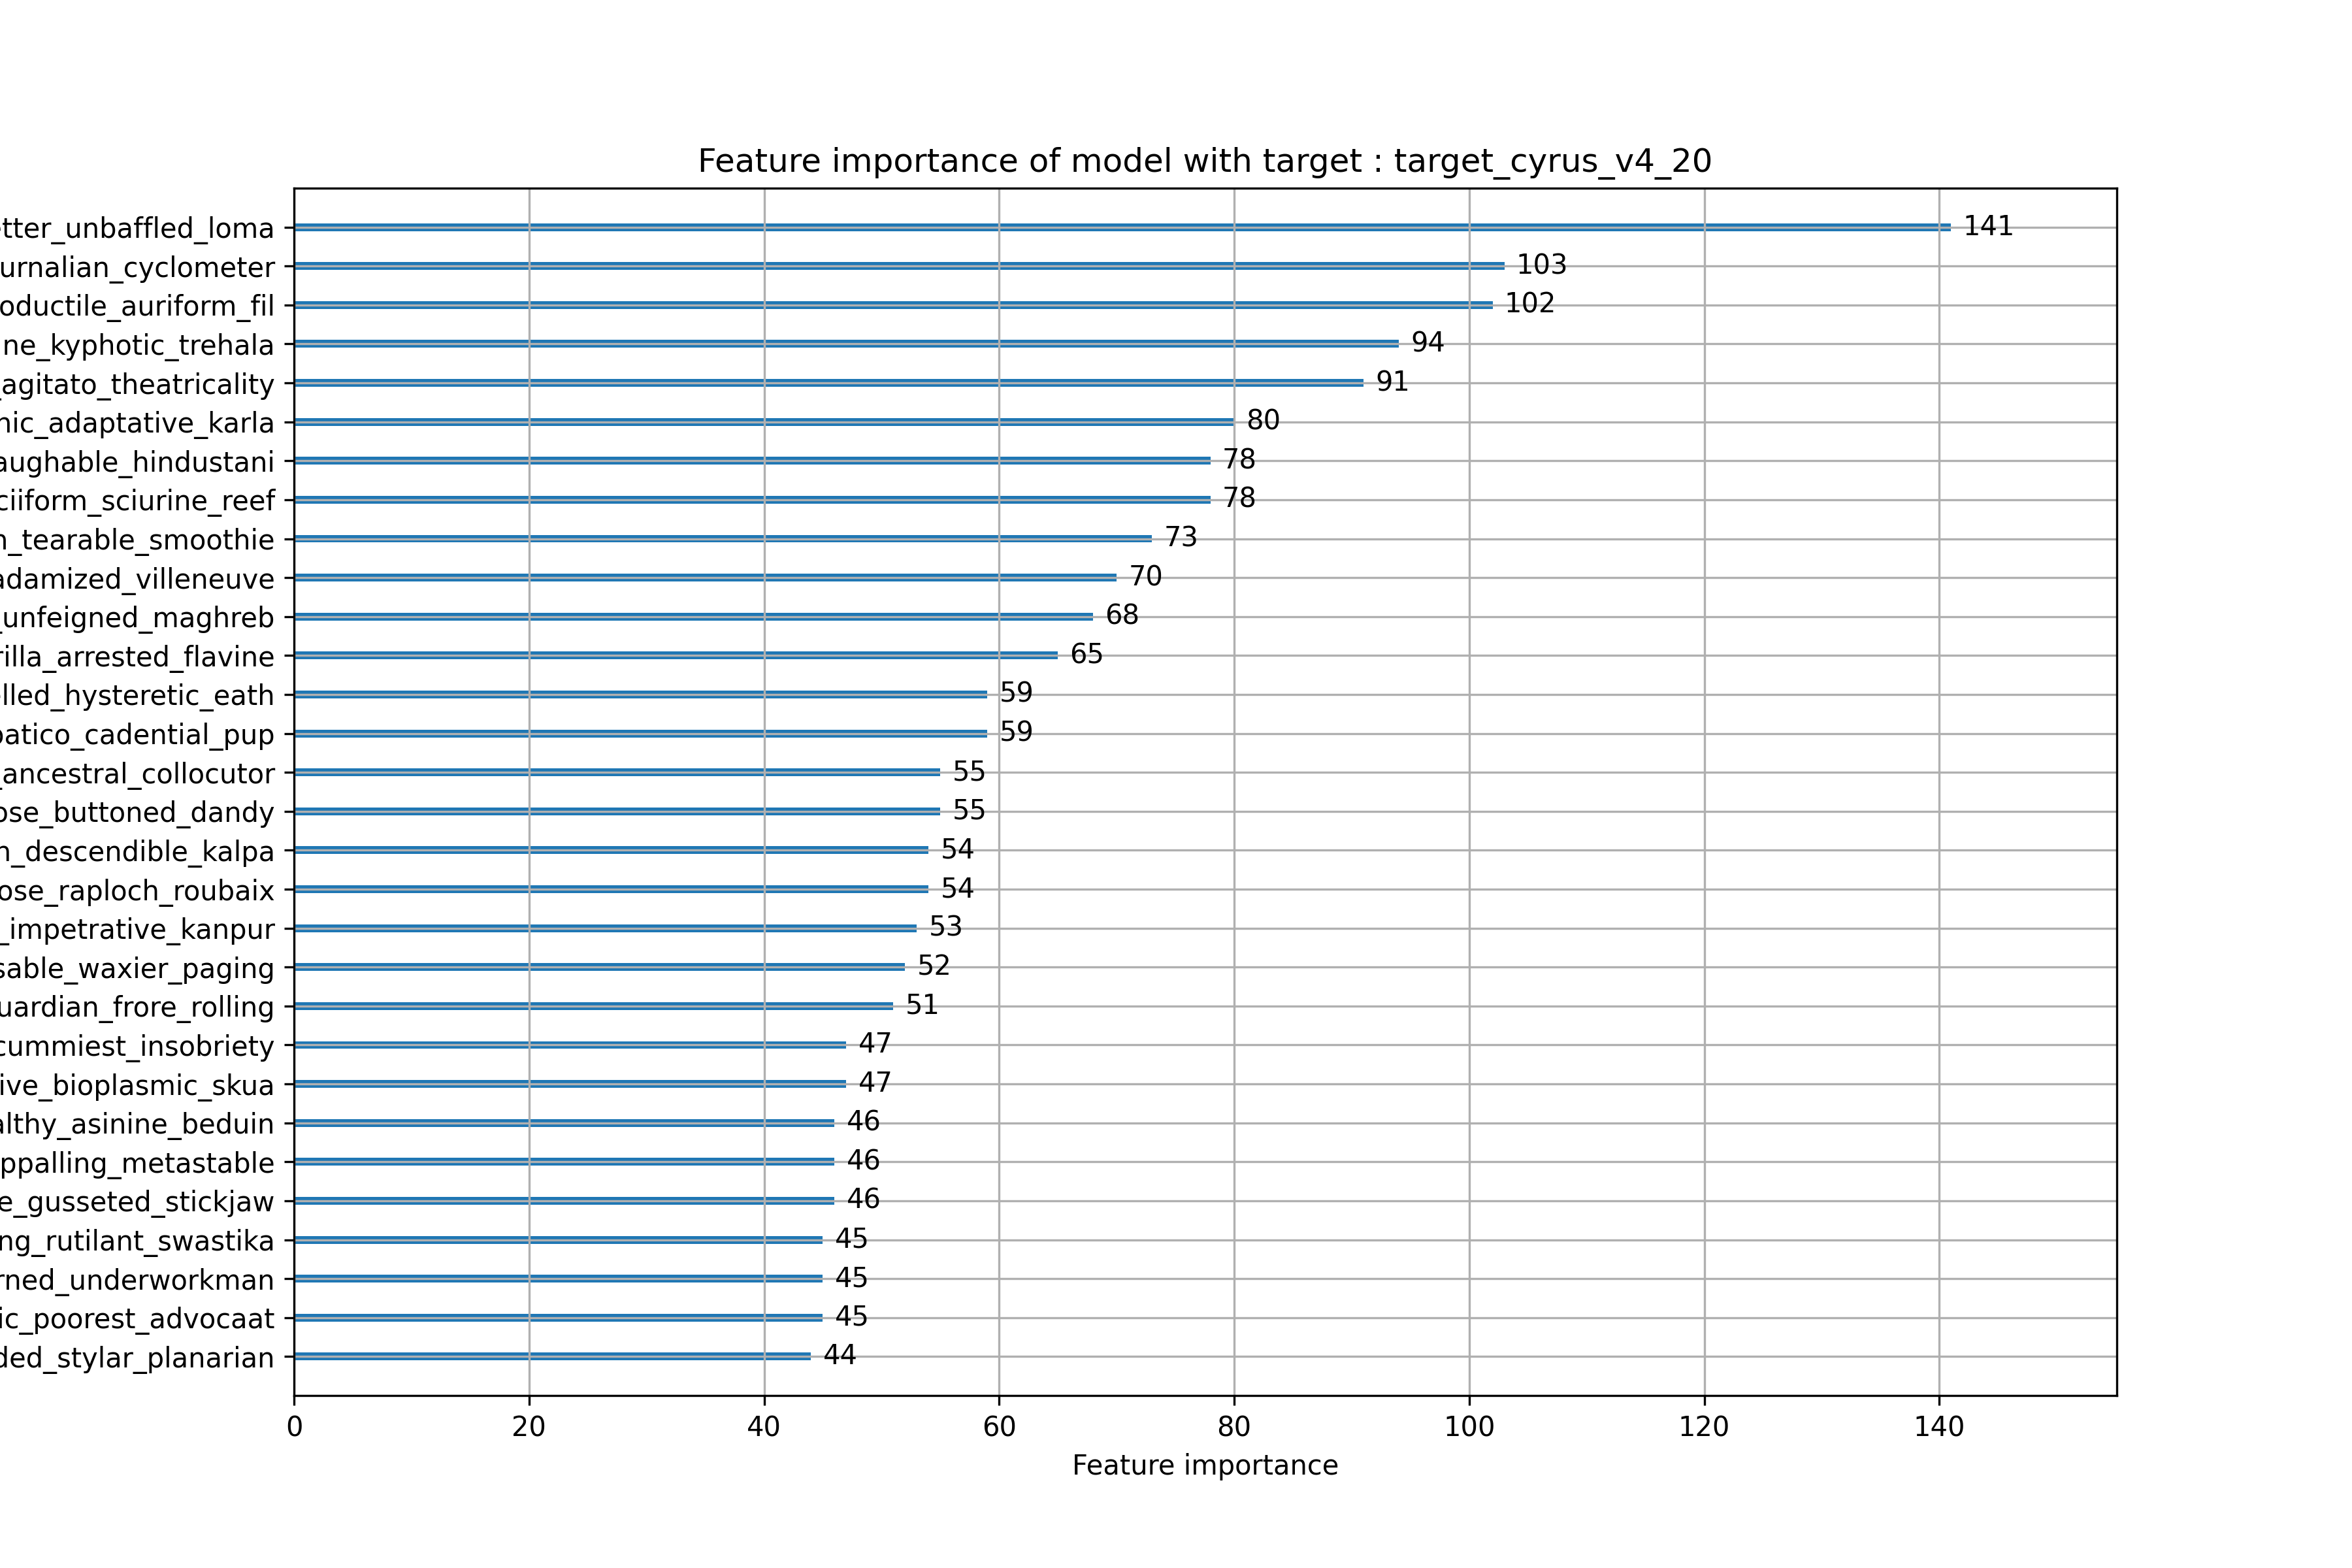
\includegraphics[width=1\textwidth,trim={0 0 0 0},clip]{figures/2023-09-28_round2_feature_importance_target_cyrus_v4_20.png}
\caption[Feature importance of model cyrus]{Feature importance of model \textit{cyrus} }
\label{fig: fi_cyrus}  
\end{minipage}
\hfill
\begin{minipage}[t]{7cm}
\vspace{0pt}
\centering
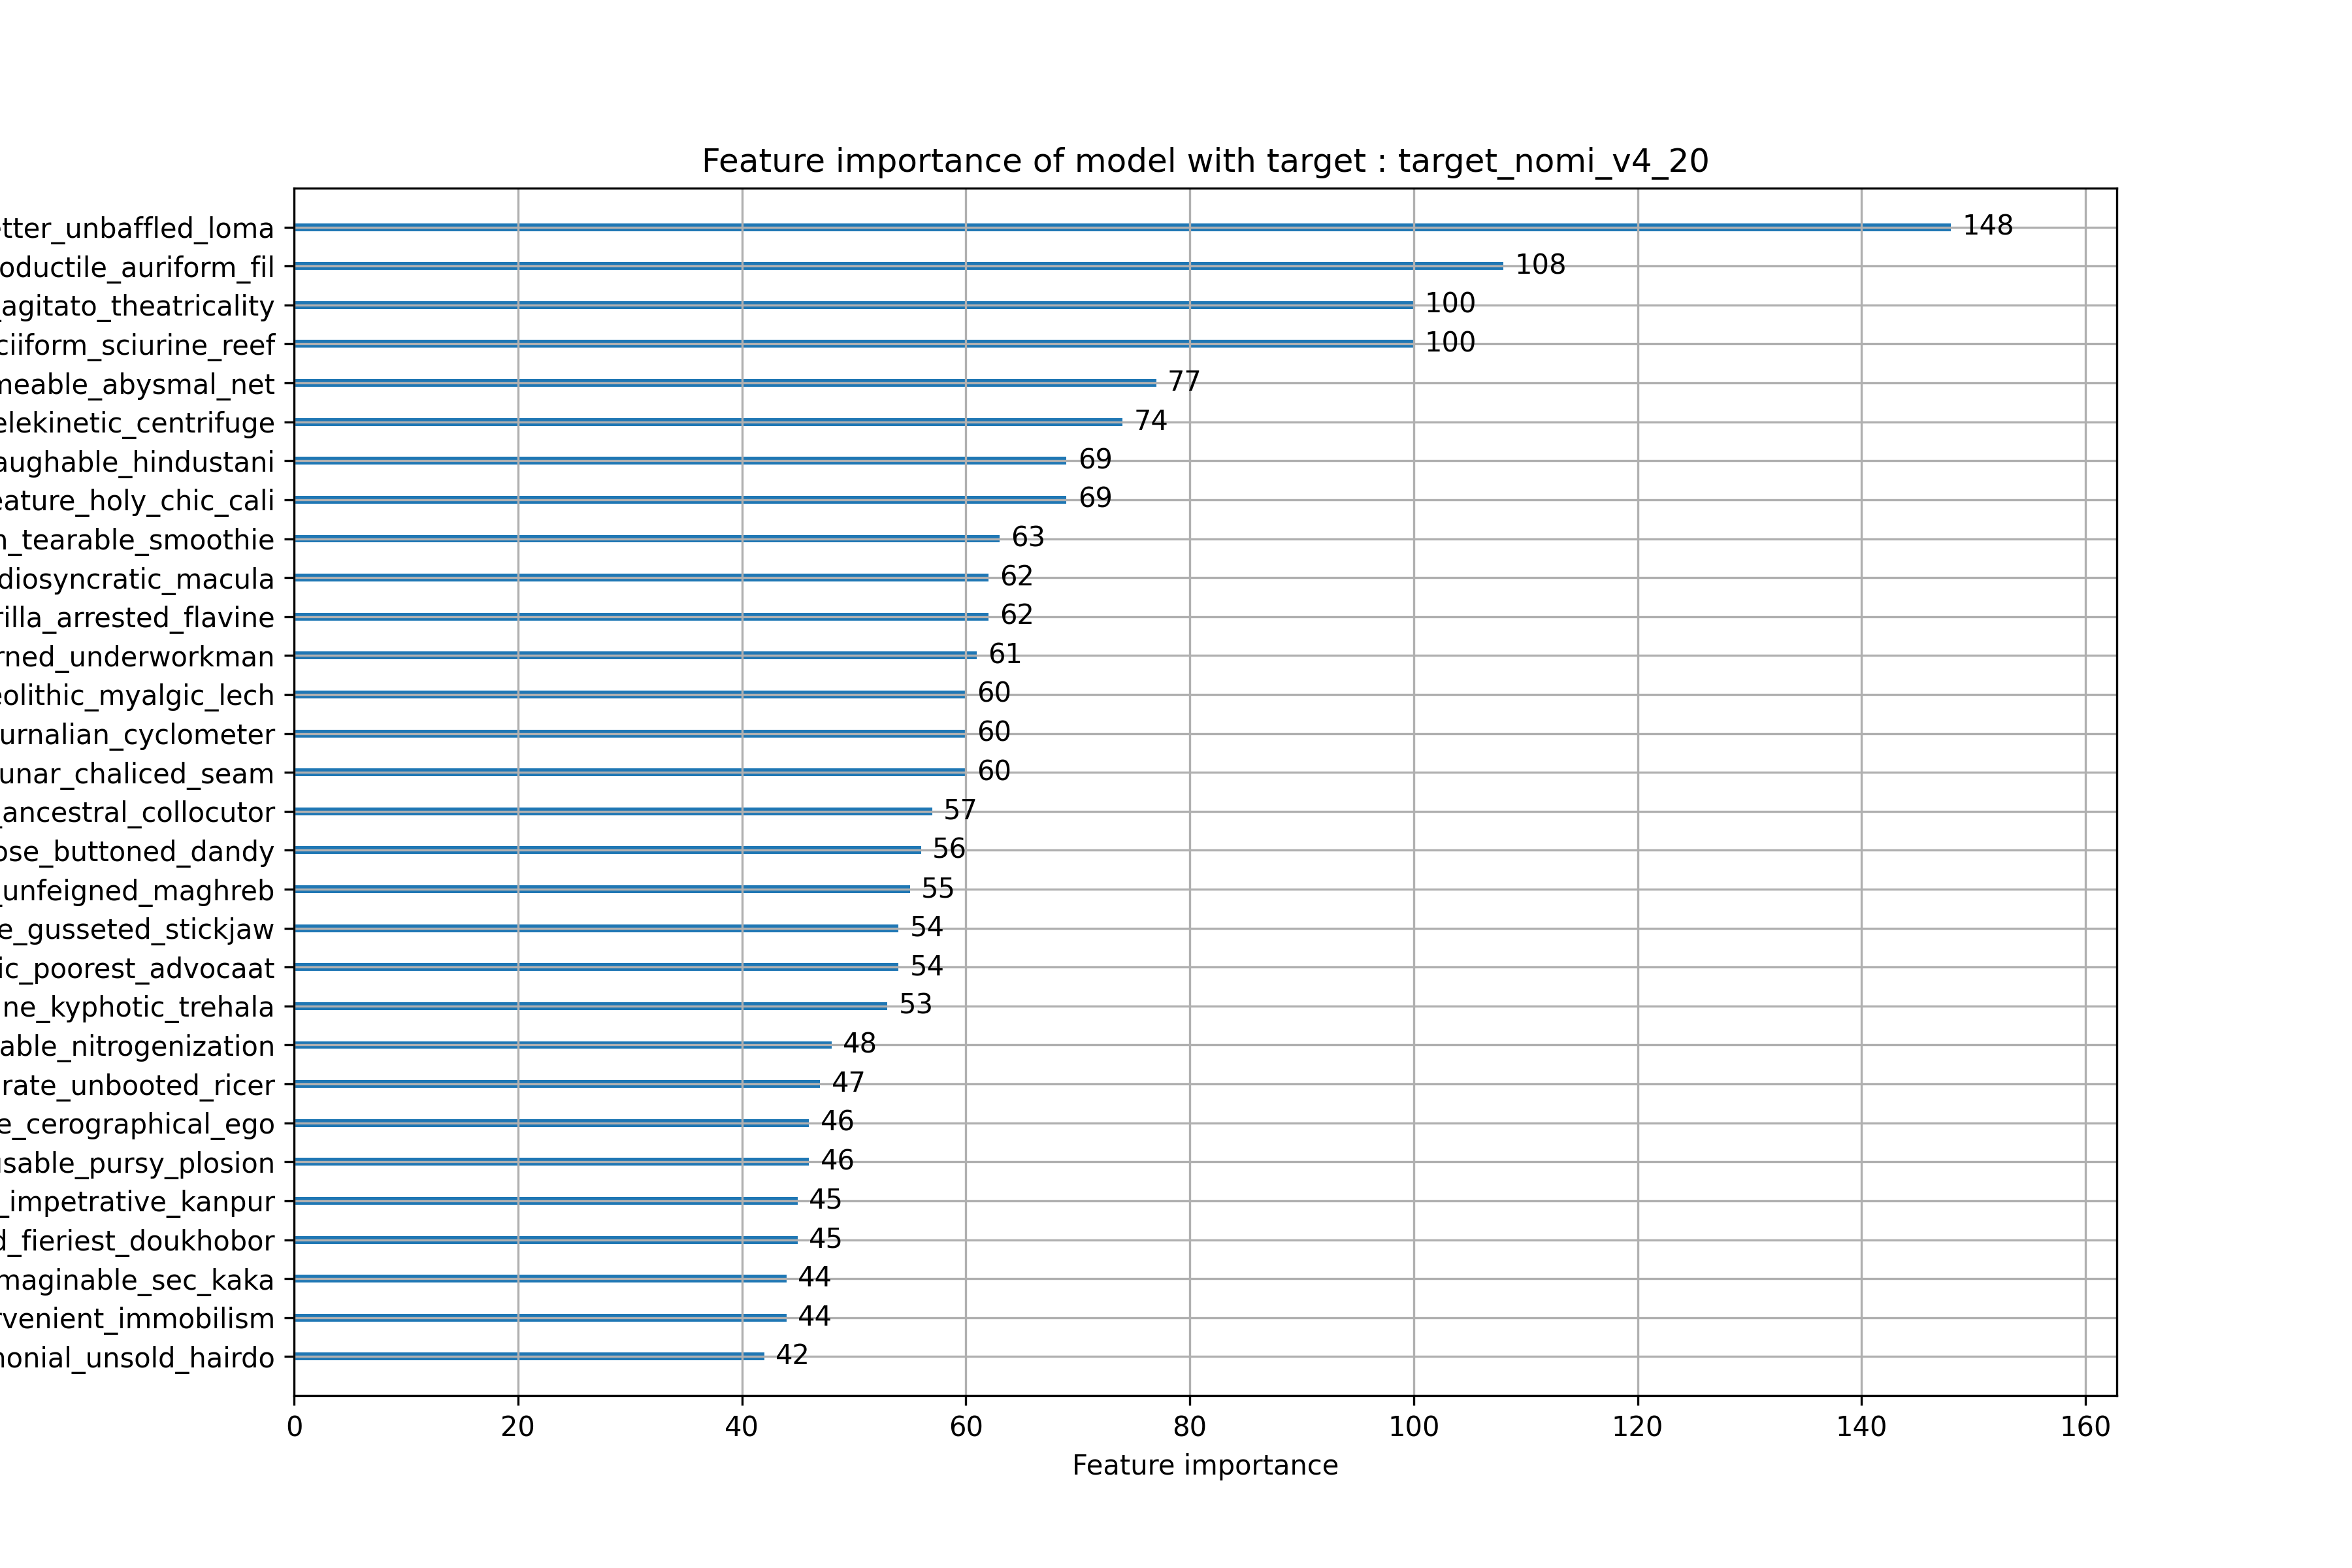
\includegraphics[width=1\textwidth,trim={0 0 0 0},clip]{figures/2023-09-28_round2_feature_importance_target_nomi_v4_20.png}
\caption[Feature importance of model nomi]{Feature importance of model \textit{nomi} }
\label{fig: fi_nomi}  
\end{minipage}
\end{figure}
We can obtain that on all models except \textit{alan} the most important feature in the weighting process is \textit{wetter unbaffled loma}. 
At model \textit{alan} this feature is ranked on place 2, whereby feature \textit{illuvial algebraic modem} is here top ranked. Interestingly this feature do not even appear in first 30 most important features of the other models. Models which rely on different important features do not tend to overestimate single features in their prediction ability. Therefor the feature exposure of the ensemble model is held low.
\begin{figure}[htbp]
\begin{minipage}[t]{7cm}
\vspace{0pt}
\centering
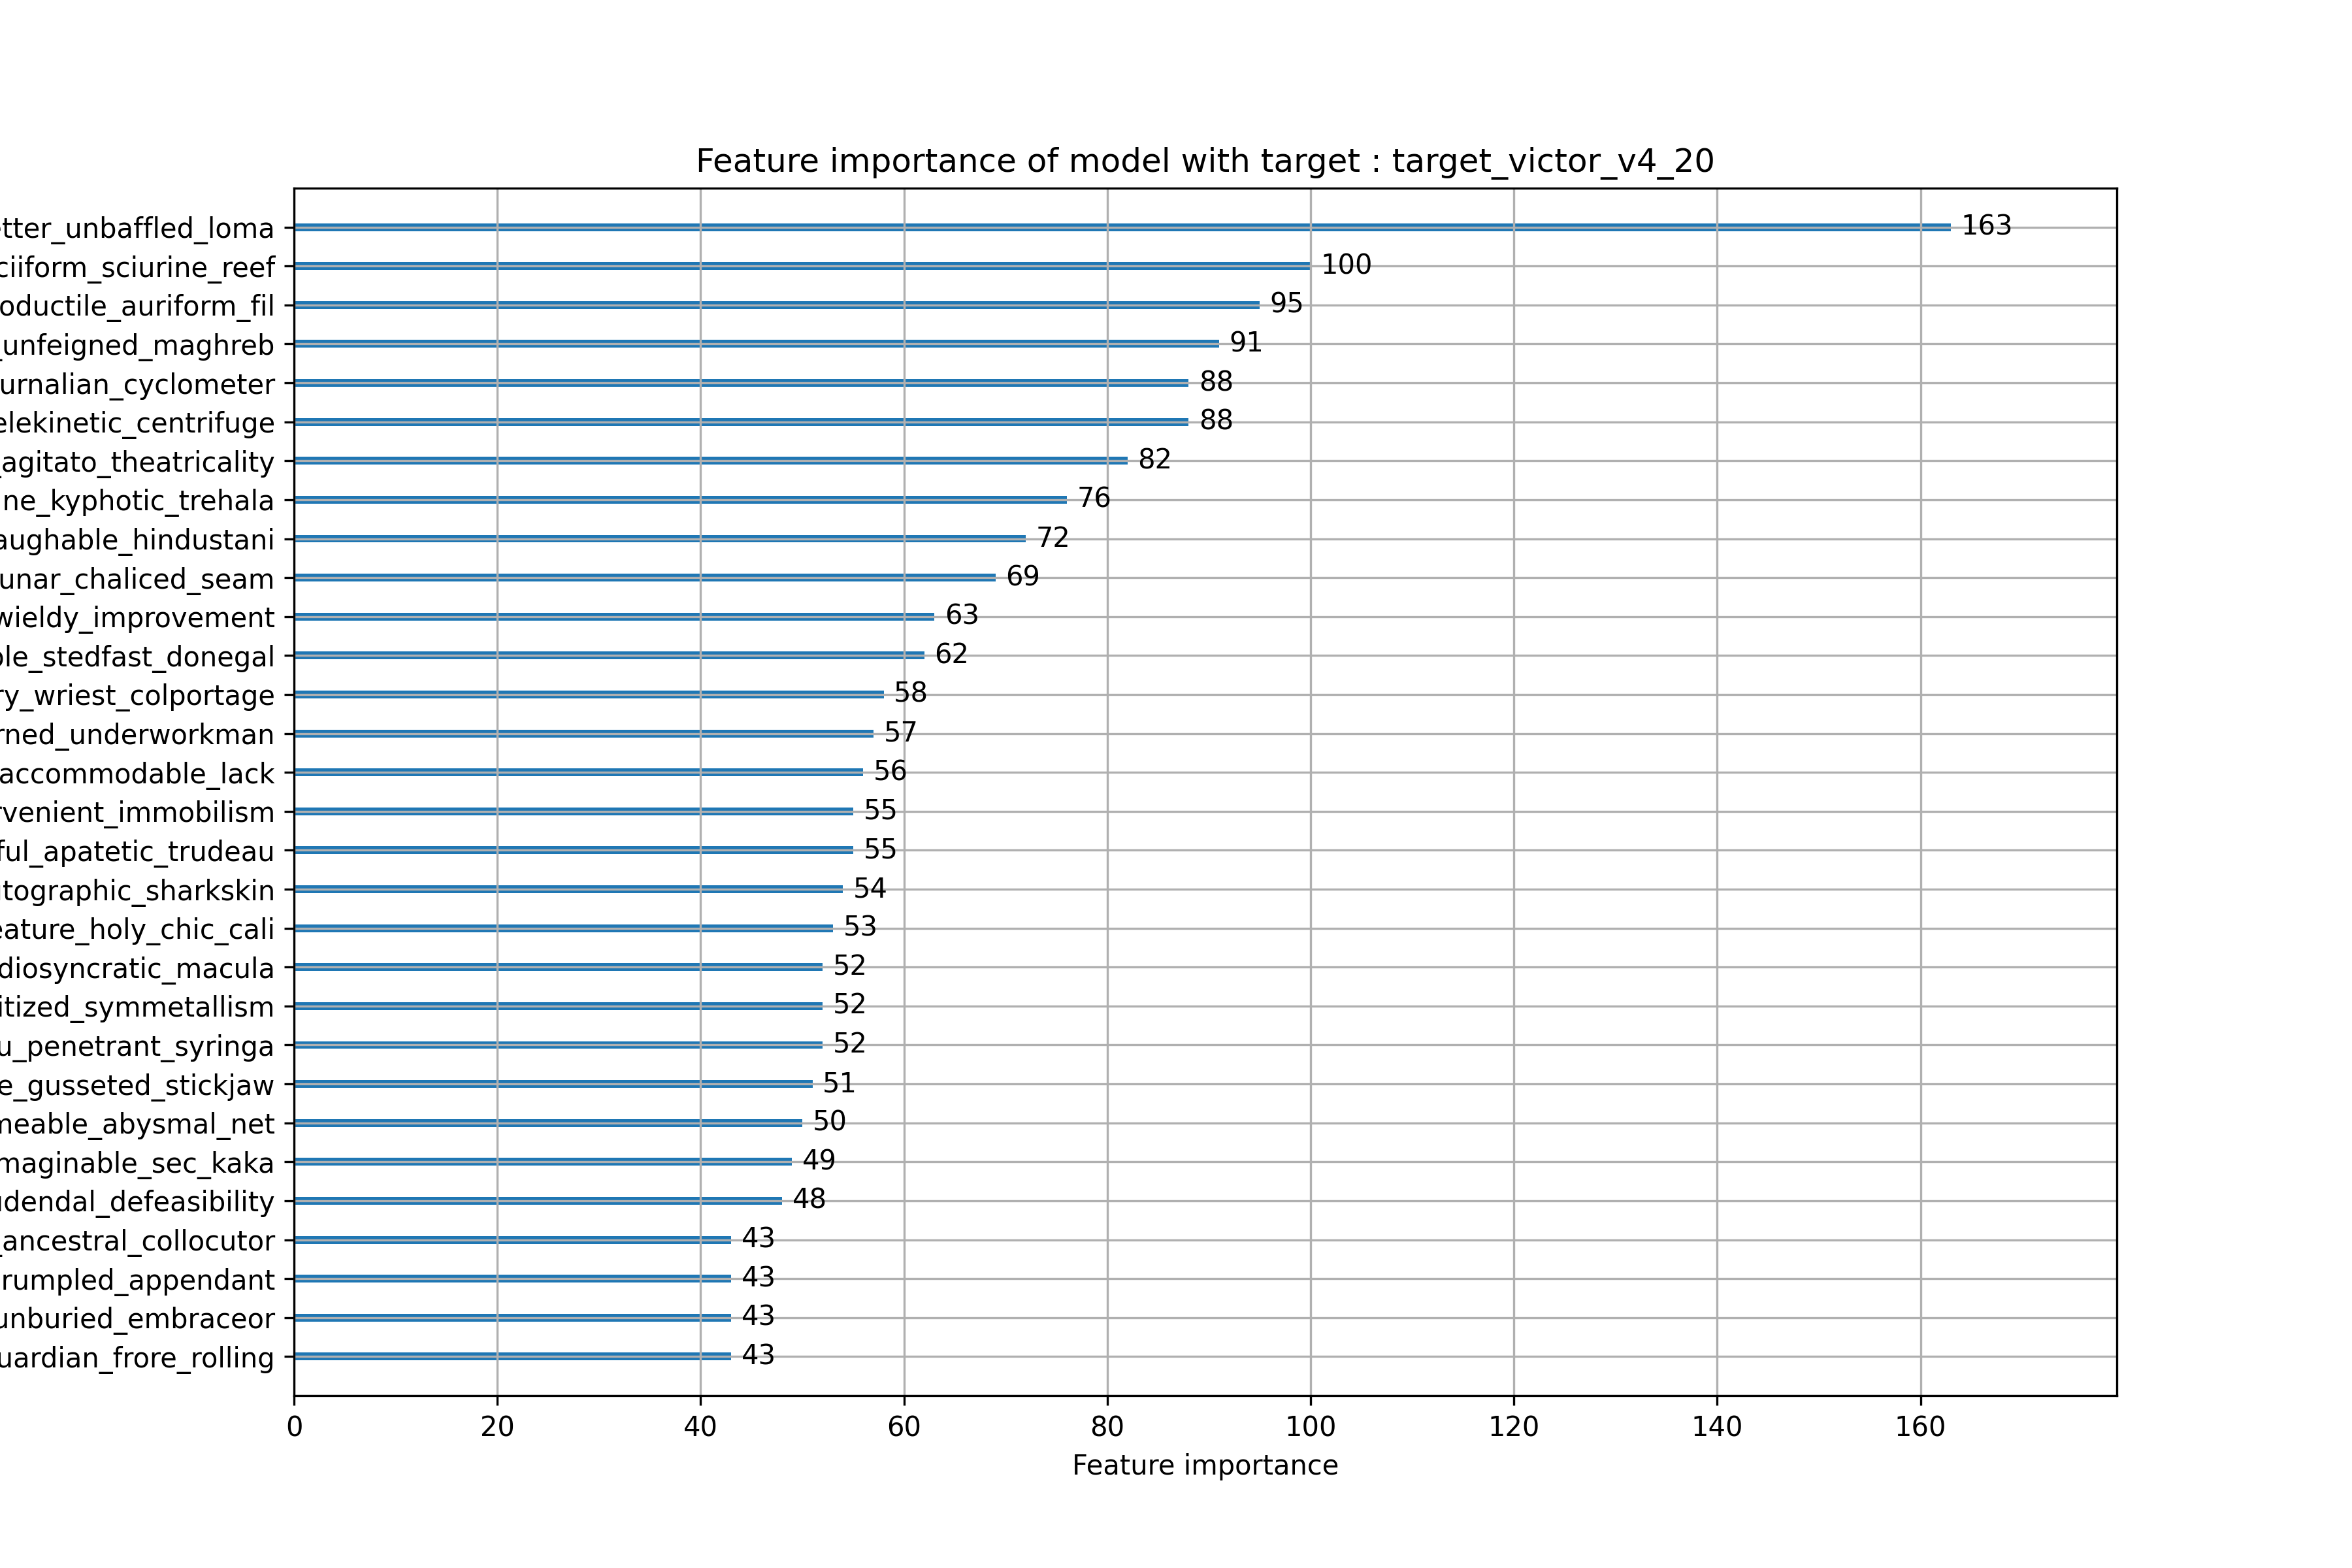
\includegraphics[width=1\textwidth,trim={0 0 0 0},clip]{figures/2023-09-28_round2_feature_importance_target_victor_v4_20.png}
\caption[Feature importance of model victor]{Feature importance of model \textit{victor} }
\label{fig: fi_victor}  
\end{minipage}
\hfill
\begin{minipage}[t]{7cm}
\vspace{0pt}
\centering
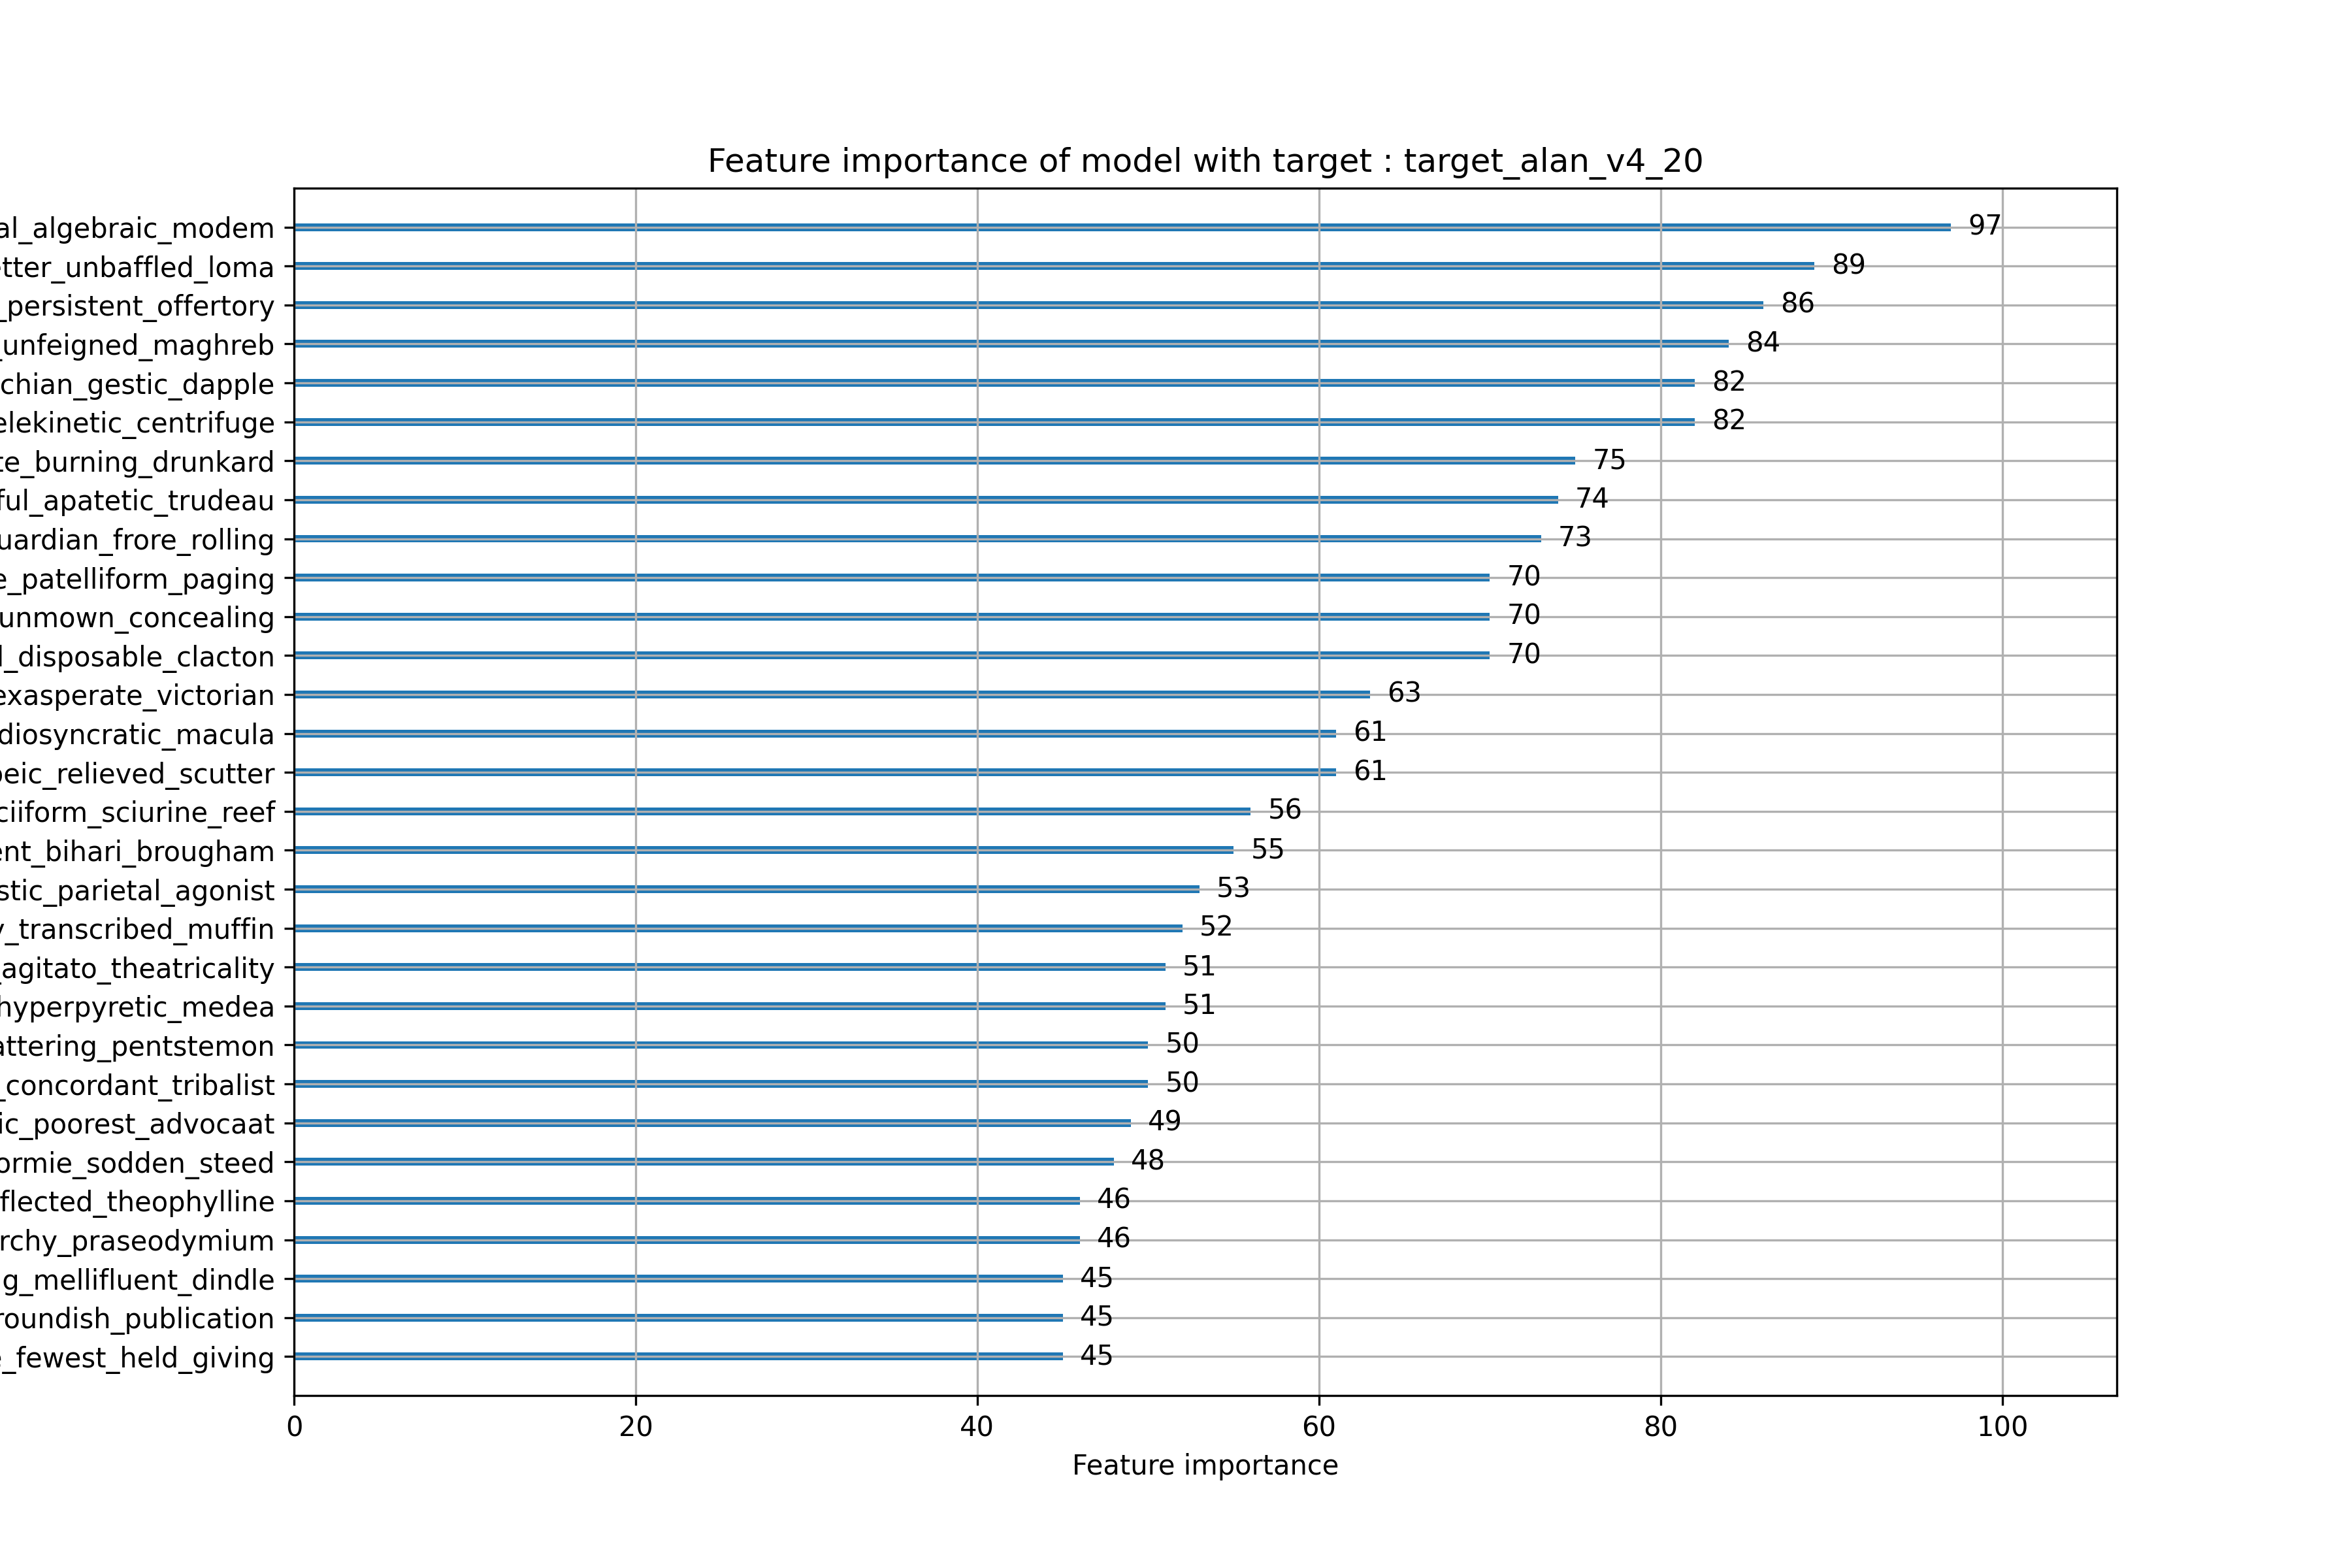
\includegraphics[width=1\textwidth,trim={0 0 0 0},clip]{figures/2023-09-28_round2_feature_importance_target_alan_v4_20.png}
\caption[Feature importance of model alan]{Feature importance of model \textit{alan} }
\label{fig: fi_alan}  
\end{minipage}
\end{figure}
%%%%%%%%%%%%%%%%%%%%%%%%%%%%%%%%%%%%%%%%%%%%%%%%%%%%%%%%%%%%%
We'll use those four GBM$^{\ast}$ models to create the ensemble model. As stated the model weights $\omega_i$ will be set all equally to $\frac{1}{4}$ and the resulting prediction values $\tilde{y}$ will be ranked by percentile because of normalization. In the following table [\ref{table: summary_metric_predictions_ensemble}] the summary metrics of ensemble model is given. For solid comparison the individual predictions as in table [\ref{table: summary_metric_predictions}] is given again.
%%%%%%%%%%%%%%%%%%%%%%%%%%%%%%%%%%%%%%%%%%%%%%%%%%%%%%%%%%%%%
\begin{table}[!htbp]
\centering
\caption{Summary metrics of prediction values from the ensemble model and different targets \\
predicted target values $\tilde{y}_i(\vec{x})$ \\
standard deviation of the predicted targets $\sigma_i(\vec{x})$ \\
sharpe ratio $S_i$ (\ref{eq: sharpe_ratio}) with risk free yield 0 \% \\
maximum drawdown $MDD$ (\ref{eq: mdd}) \\
mean correlation $C_{iCyrus}$ with \textit{target cyrus} \\}
\label{table: summary_metric_predictions_ensemble}
\begin{tabular}{|l|l|l|l|l|l|}
\hline
\textit{targets} & mean[$\tilde{y}_i(\vec{x})$] & $\sigma_i(\vec{x})$ & $S_i$ & $MDD$ & $C_{iCyrus}$ \\ \hline
\hline
\hline
\textit{cyrus} & 0,0191 & 0,0207 & 0,9214 & 0,0510 & 1,0  \\ \hline
\textit{alan} & 0,0107 & 0,0213 & 0,4995 & 0,1000 & 0,6650 \\ \hline
\textit{nomi} & 0,0191 & 0,0207 & 0,9217 & 0,0393 & 0,8248 \\ \hline
\textit{victor} & 0,0184 & 0,0187 & 0,9852 & 0,0456 &  0,8290 \\ \hline
\hline
\textit{ensemble} & 0,0189 & 0,0202 & 0,9377 & 0,0504 & 0,9234 \\ \hline
\end{tabular}
\end{table}
Lastly the cumulative correlation of validation predictions is shown again in figure [\ref{fig: cum_corr_val_preds_ensemble}].
\begin{figure}[!htpb]
    \centering
    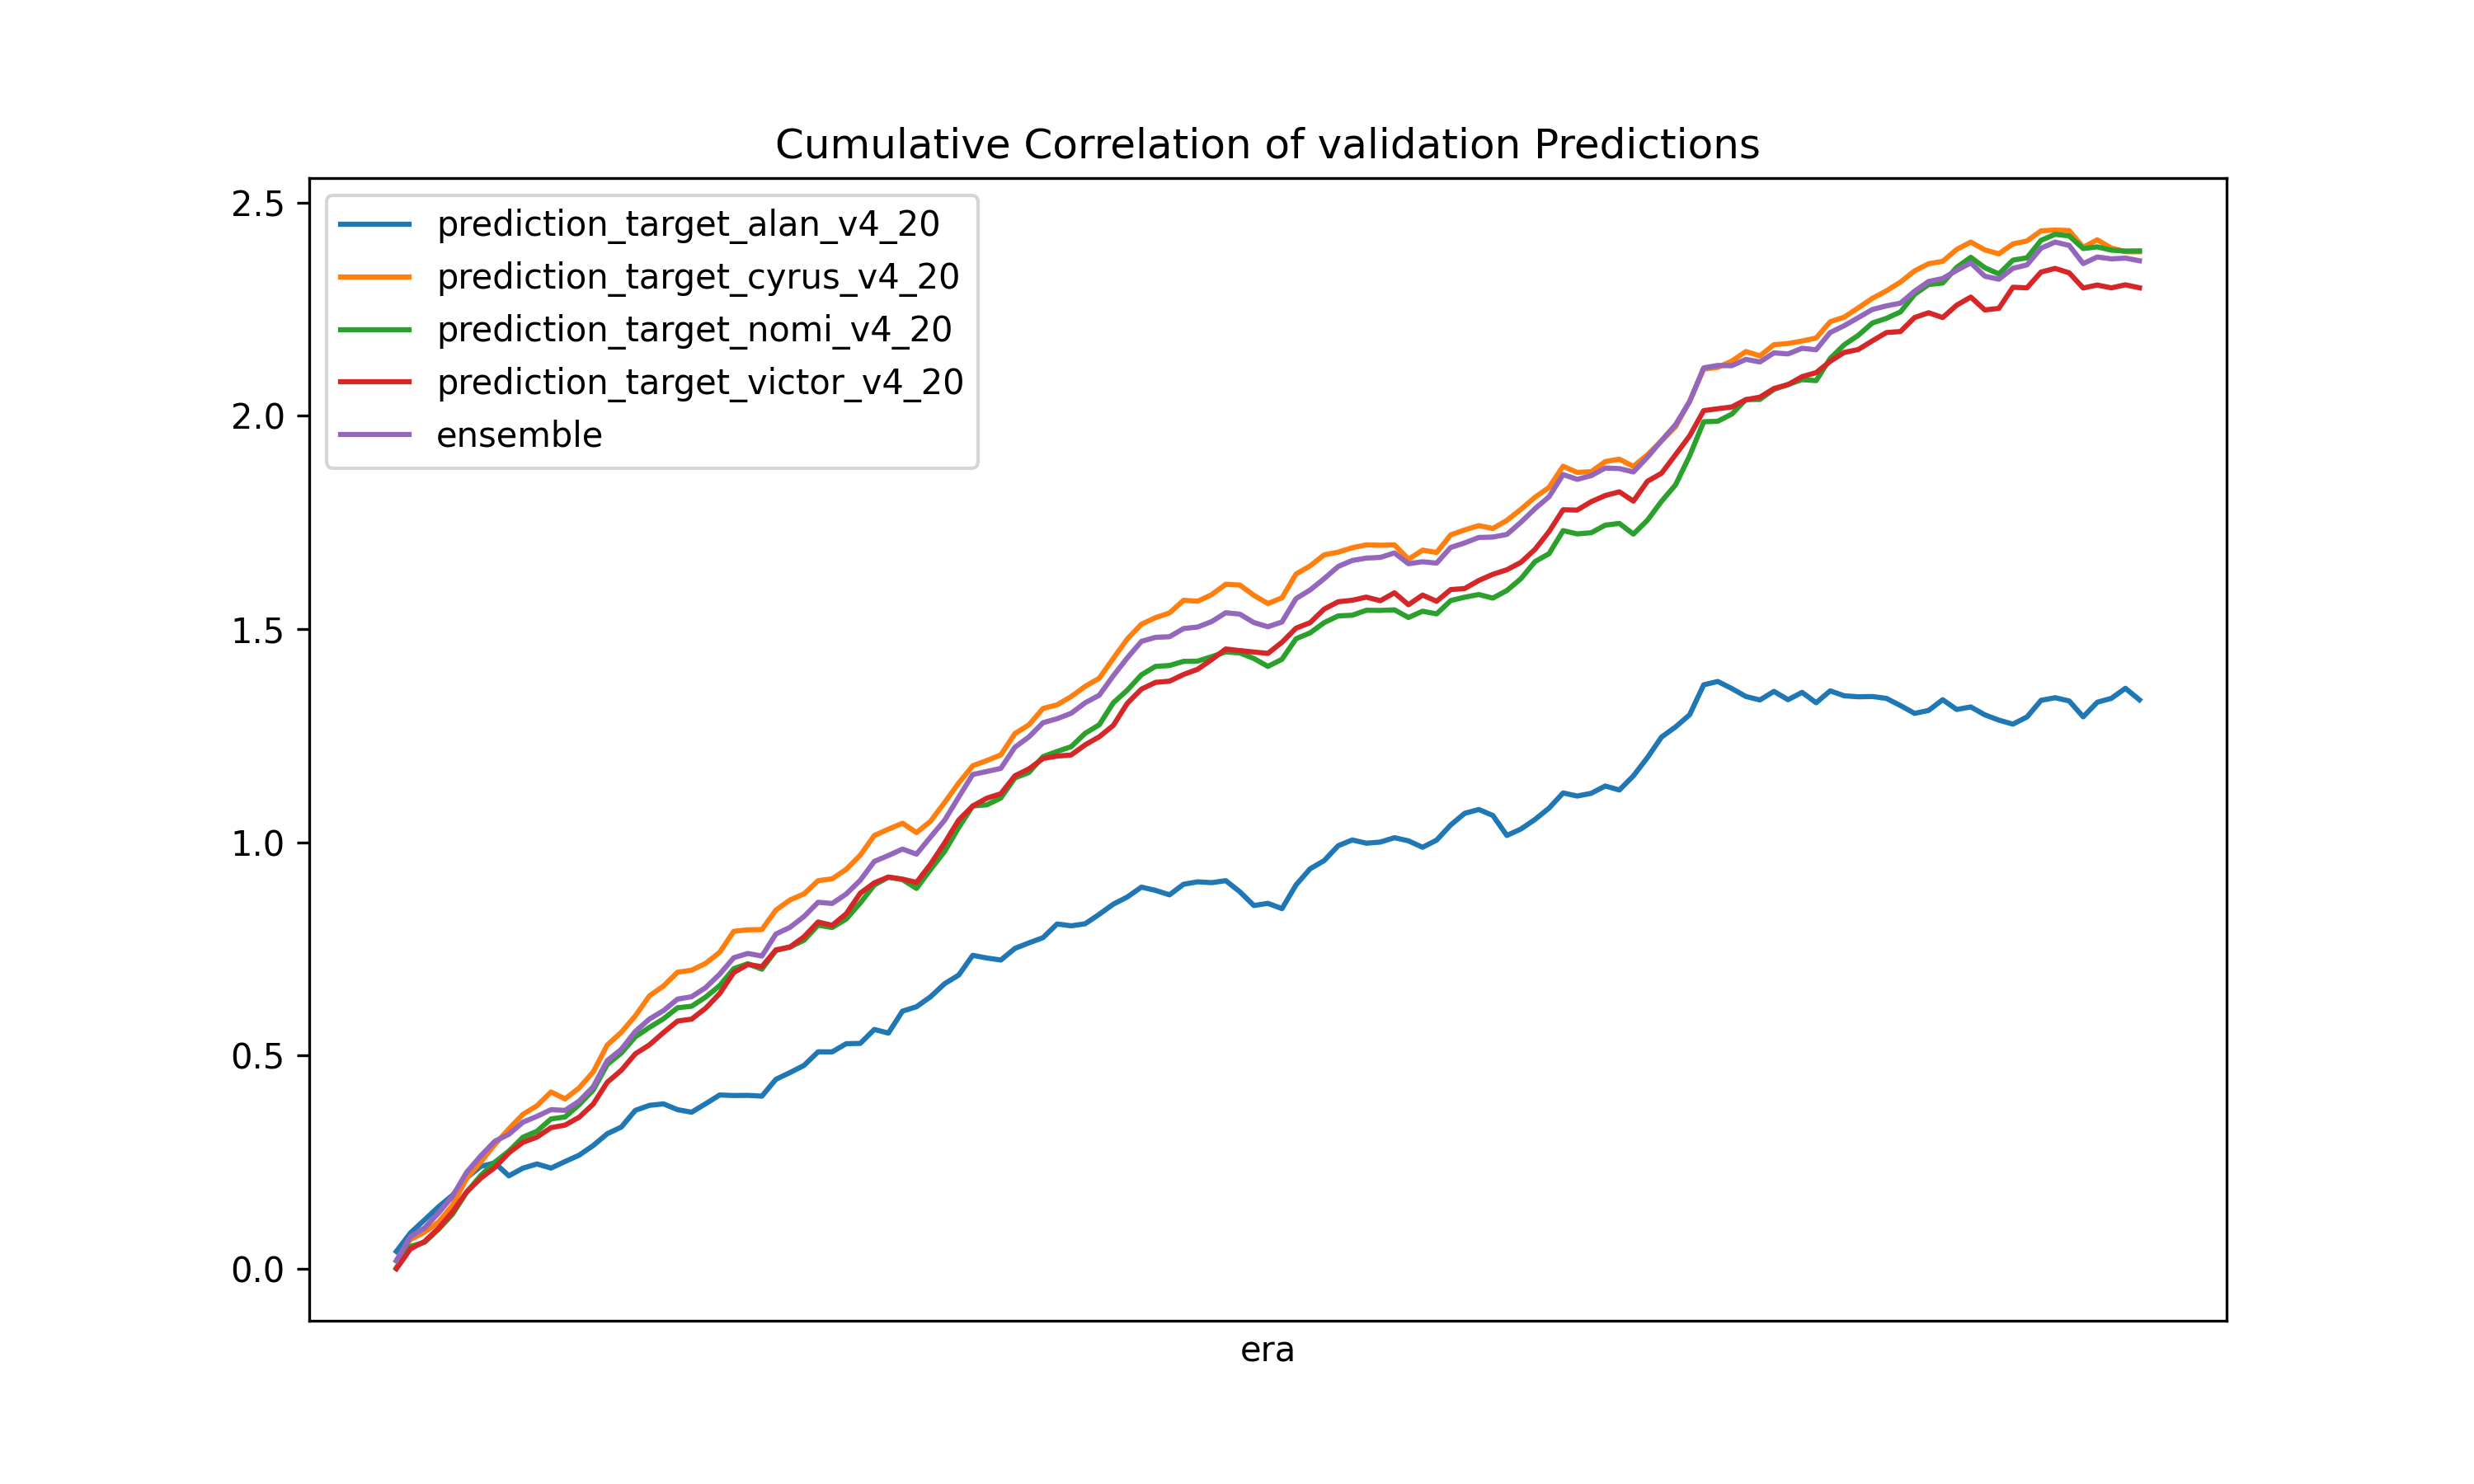
\includegraphics[width=1\textwidth,trim={0 0 0 0},clip]{figures/2023-09-28_round2_cumulative_correlation_of_validation_predicitions_ensemble.png}
    \caption[Cumulative per era correlation of validation predictions over the GBM$^{\ast}$ ensemble model with comparison]{Cumulative per era correlation of validation predictions $\tilde{y}(\vec{x}(t))$ over the GBM$^{\ast}$ ensemble model with comparison}
    \label{fig: cum_corr_val_preds_ensemble}    
\end{figure}
\\
As stated in section [\ref{sec: neutralizing}] feature neutralization can be a very important step towards a better behaving model over the long run. \href{https://numer.ai}{Numer.ai} proposes here an elegant way to reduce the feature exposure by neutralizing a whole feature group [Fig. \ref{fig: cum_corr_val_preds_ensemble_neutral}]. 
\begin{figure}[!htpb]
    \centering
    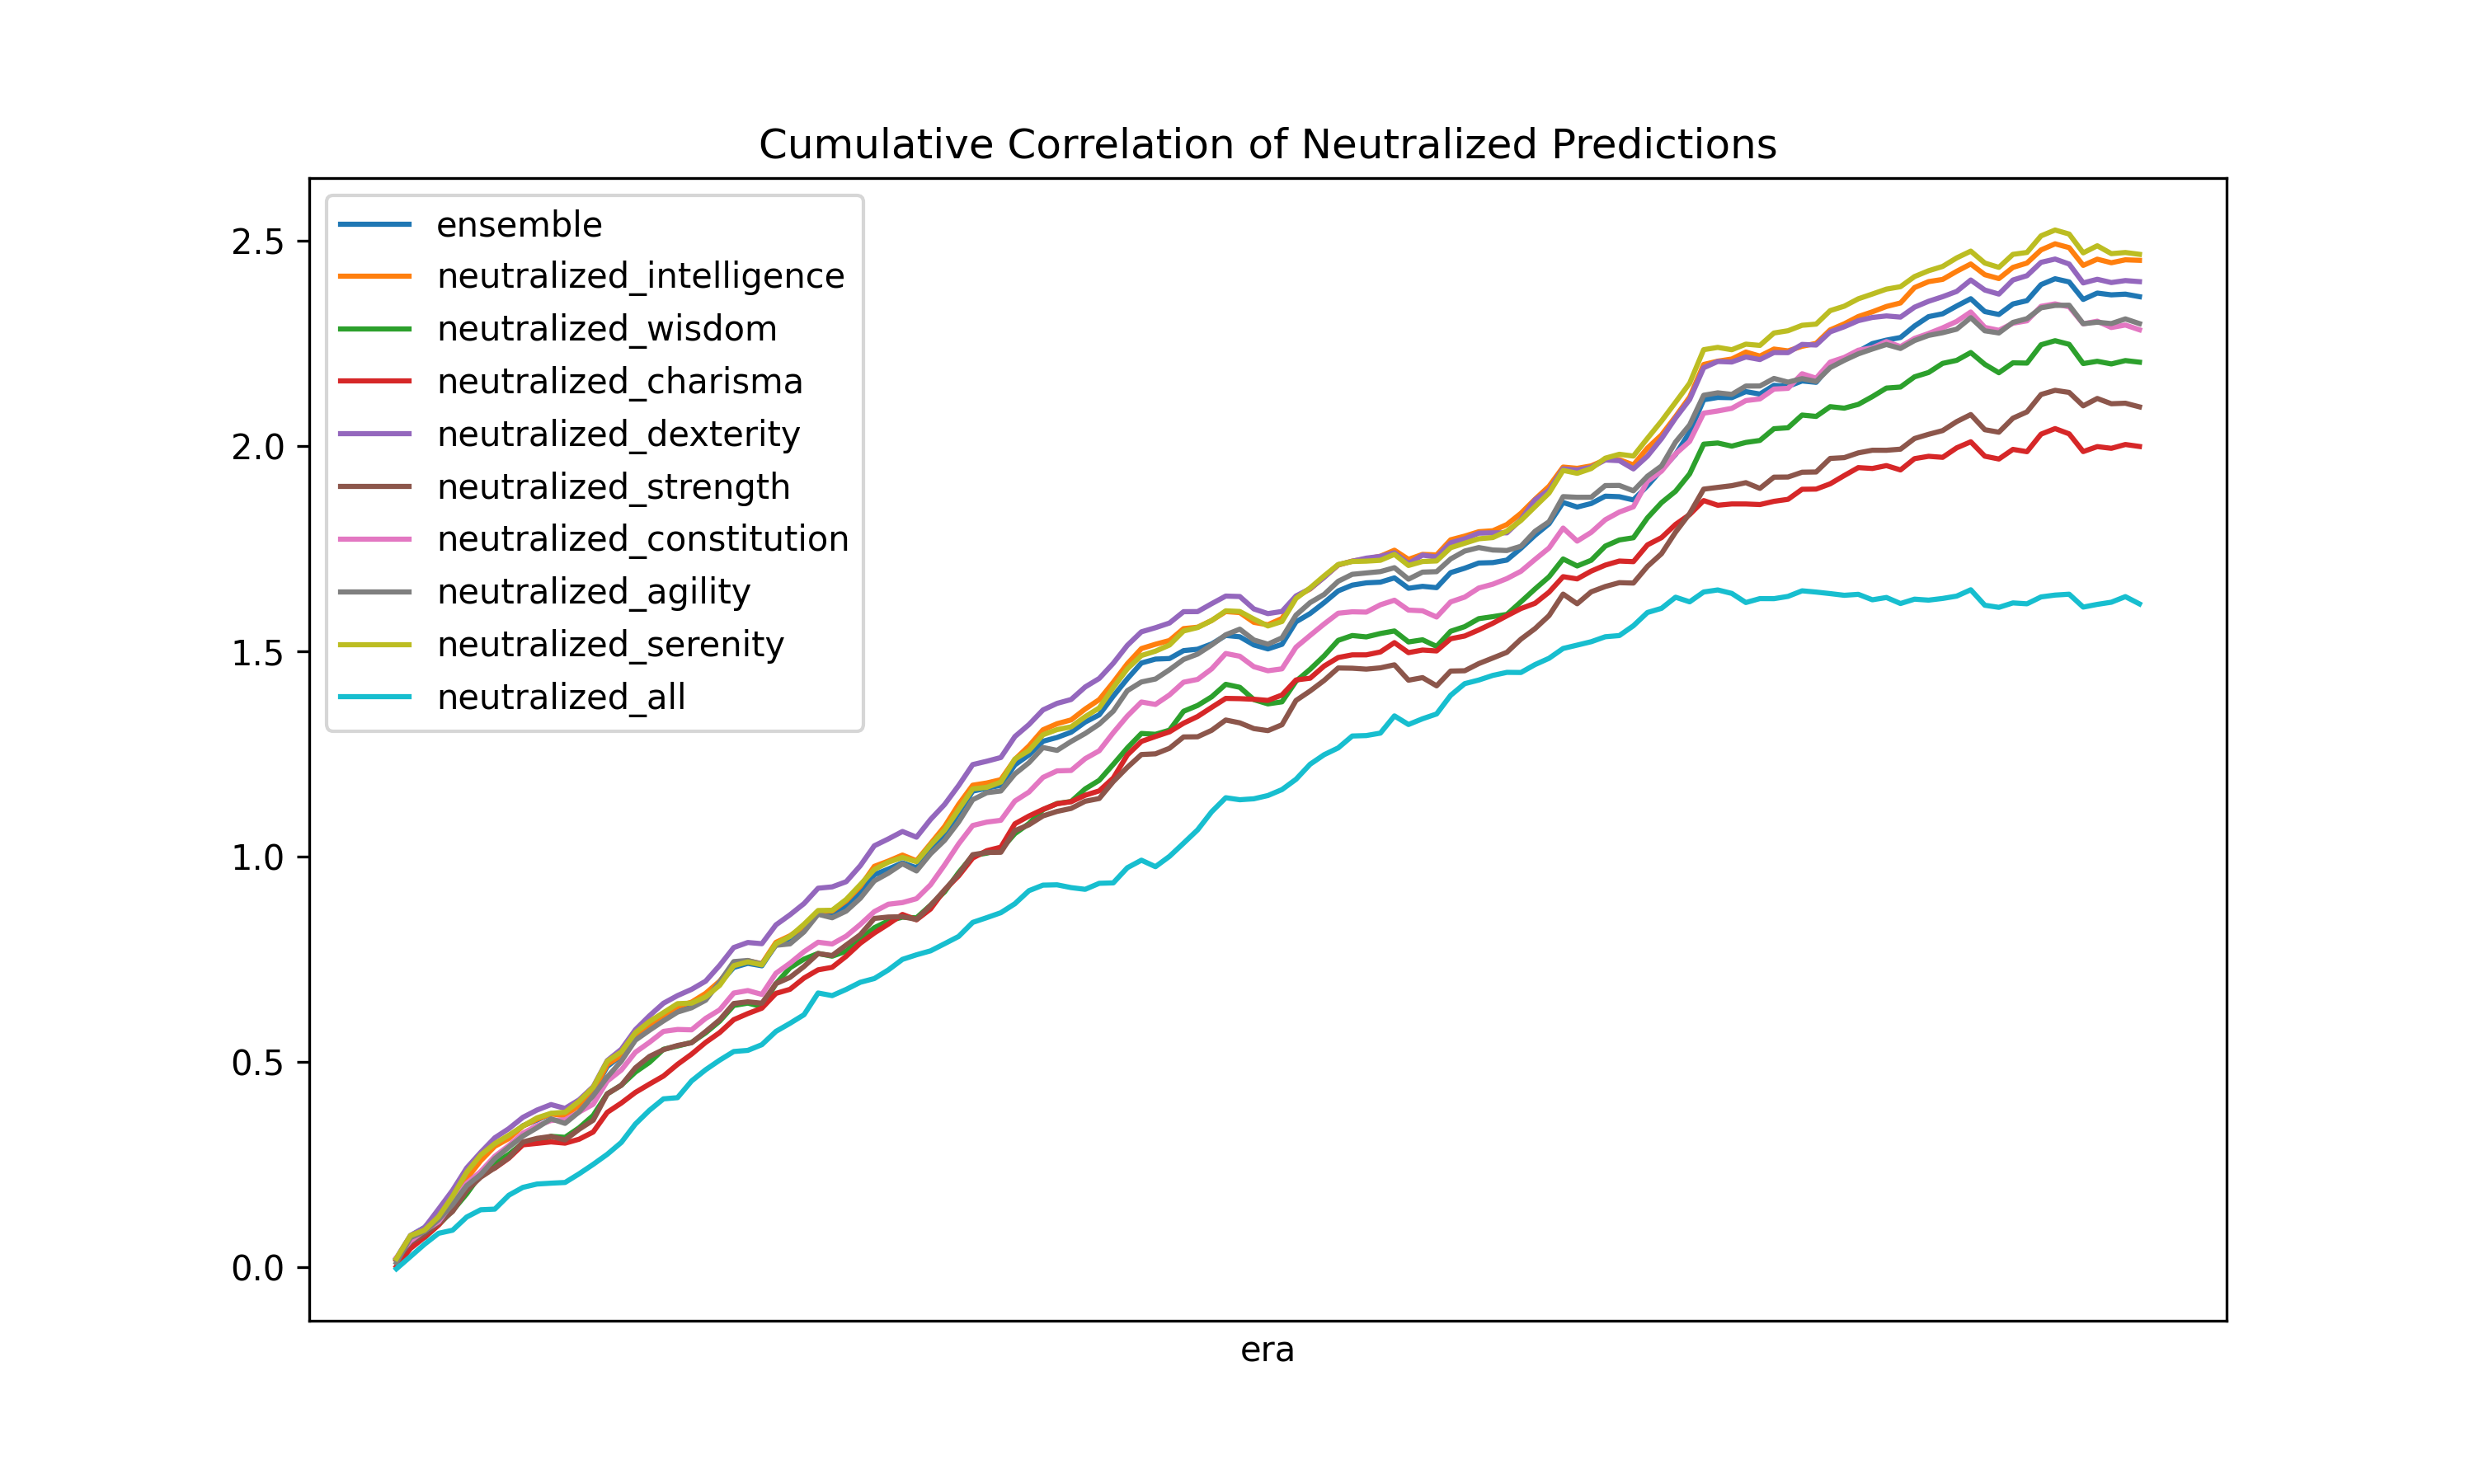
\includegraphics[width=1\textwidth,trim={0 0 0 0},clip]{figures/2023-10-01_round4_cumulative_correlation_of_validation_predicitions_neutralization_ensemble.png}
    \caption[Cumulative per era correlation of neutralized predictions of the GBM$^{\ast}$ ensemble model with comparison]{Cumulative per era correlation of neutralized validation predictions $\tilde{y}(\vec{x}(t))$ of the GBM$^{\ast}$ ensemble model with comparison}
    \label{fig: cum_corr_val_preds_ensemble_neutral}    
\end{figure}
We can see that by neutralizing the feature group \textit{serenity} one gets the best per era correlation within the target. Projecting this one the per era correlation of the whole \textit{serenity} group which was plotted in figure [\ref{fig: per_era_correlation}] one can definitely obtain features with higher fluctuations and less per era correlation. So by neutralizing this feature group the specific feature exposure will be reduced. Consequently consistency in the predictions by the model will be increased and therefor the scoring ratios as shown in table [\ref{table: summary_metric_predictions_neutral_ensemble}]. \\
It is clearly evident that the sharpe ratio results in a higher value of $S_{n.Ens.} = 0,9546$ over the given timeperiod (eras). The higher volatility $\sigma_{n.Ens.}(\vec{x})$ of the neutralized ensemble model induces also a higher maximum drawdown $MDD$ which ultimately results in such a behavior. \\
Another optimization of the model would be the neutralization of multiple feature groups instead of a single one. One would argue that if two seperated groups give better predictions results than the ensemble model solely, neutralizing multiple groups can only lead to better performance. 
\newpage 
But one has to keep in mind that due the fact that the dataset gets updated weekly this might change over time. Therefor the continuously review of the model performance is mandatory for getting consistent results.
With this model one can get descent results on this financial prediction problem which was provided by \href{https://numer.ai}{numer.ai}. 
\begin{table}[!htbp]
\centering
\caption{Summary Metrics of prediction values from the ensemble and neutralized ensemble model \\
predicted target values $\tilde{y}_i(\vec{x})$ \\
standard deviation of the predicted targets $\sigma_i(\vec{x})$ \\
sharpe ratio $S_i$ (\ref{eq: sharpe_ratio}) with risk free yield 0 \% \\
maximum drawdown $MDD$ (\ref{eq: mdd}) \\
mean correlation $C_{iCyrus}$ with \textit{target cyrus} \\}
\label{table: summary_metric_predictions_neutral_ensemble}
\begin{tabular}{|l|l|l|l|l|l|}
\hline
\textit{targets} & mean[$\tilde{y}_i(\vec{x})$] & $\sigma_i(\vec{x})$ & $S_i$ & $MDD$ & $C_{iCyrus}$ \\ \hline
\hline
\hline
\textit{ensemble} & 0,0189 & 0,0202 & 0,9377 & 0,0504 & 0,9234 \\ \hline
\hline
\textit{neutral. ensemble} & 0,0197 & 0,0207 & 0,9546 & 0,0592 & 0,9421 \\ \hline 
\end{tabular}
\end{table}

\newpage
\section{Conclusion}
Gradient Boosting is a powerful tool in the area of supervised machine learning. In addition with Decision Trees as base learners one can create models for prediction tasks where non-linearity plays a significant role. 
Because of the design of the framework one can easily analyze the decisions which are made to split the data by the algorithm. This ``transparency`` of the system can be a huge benefit compared to other techniques like Neural Networks, which are indeed kind of ``black-box`` systems. Bayesian Optimization acts from an abstract point of view as the inner clock working for tuning the model with the right hyperparameters, which is key for finding the best possible model as shown. For prediction tasks where multiple targets are given one has to evaluate clearly which one to choose. Here is the possibility to use further informative algorithms like Bayesian Model Averaging (BMA) to dynamically adjust the current sub-models by assigning them optimal weights for the given set. Furthermore there's always the possibility to use other supervised machine learning algorithms like Neural Networks (NN), Support Vector Machines (SVM) or Random Forests (RF). \\
Finally, it must be said that due to the constant updating of the data of \href{https://numer.ai}{Numer.ai}, the evaluations will change over time.
\section{Final thoughts and acknowledgement}
First, I would like to thank my supervisor Prof. Dr. Wolfgang Von der Linden and Dr. Sascha Ranftl for giving me this opportunity to work on a present and still growing topic in the field of machine learning. Even if it's not specifically a pure physics topic the application of modern prediction algorithms can be mandatory when dealing with a huge amount of data. \\
But ultimately, and that's perhaps the most important one, I was able to
introduce and expand my knowledge, which I gathered in the past three years of studying physics, in this bachelor thesis. \\
Thanks must also go to Alexander who provided me with feedback from the
point of view of a reader that is new to this topic. Last but not least, I thank my parents Hannes and Daniela for enabling me the study of Physics in Graz. 
%%%%%%%%%%%%%%%%%%%%%%%%%%%%%%%%%%%%%%%%%%%
\newpage
\printbibliography
\newpage
\listoffigures
\end{document}